\chapter{Design}
\section*{Overview}
This section includes a breakdown of the application into sections of data processing, GUI functionalities and joint functionalities. The use of external sources including DM-D.S.S. and NIED data sources is discussed, together with the relevant formats (JSON) and the objects related. UML class diagrams are included to discuss OOP relations of classes, records (record classes) and enums including the use of inheritance, composition, association and aggregation. They also implement different interfaces. Design patterns that should be included in the application are also introduced and outlined. An outline of the design of the user interface is included. The expected hardware requirements of the systems are also listed, but any laptop with an up-to-date operating system (running Windows or macOS) should be able to run the program.

\section{Hierarchy Chart}
As discussed in the analysis section, the program consists of three parts: data-parsing from external data sources, GUI functionalities and joint functionalities, where the GUI part will be divided into two parts focusing on real-time monitoring and past-earthquake information, respectively. Here, functionalities for each particular module is further split up. Figure \ref{fig:hierarchy} is a hierarchy diagram for the whole application. This shows how \textbf{decomposition} technique is applied to reduce a sophisticated problem into more attackable problems.

\begin{figure}[htp]
    \centering
    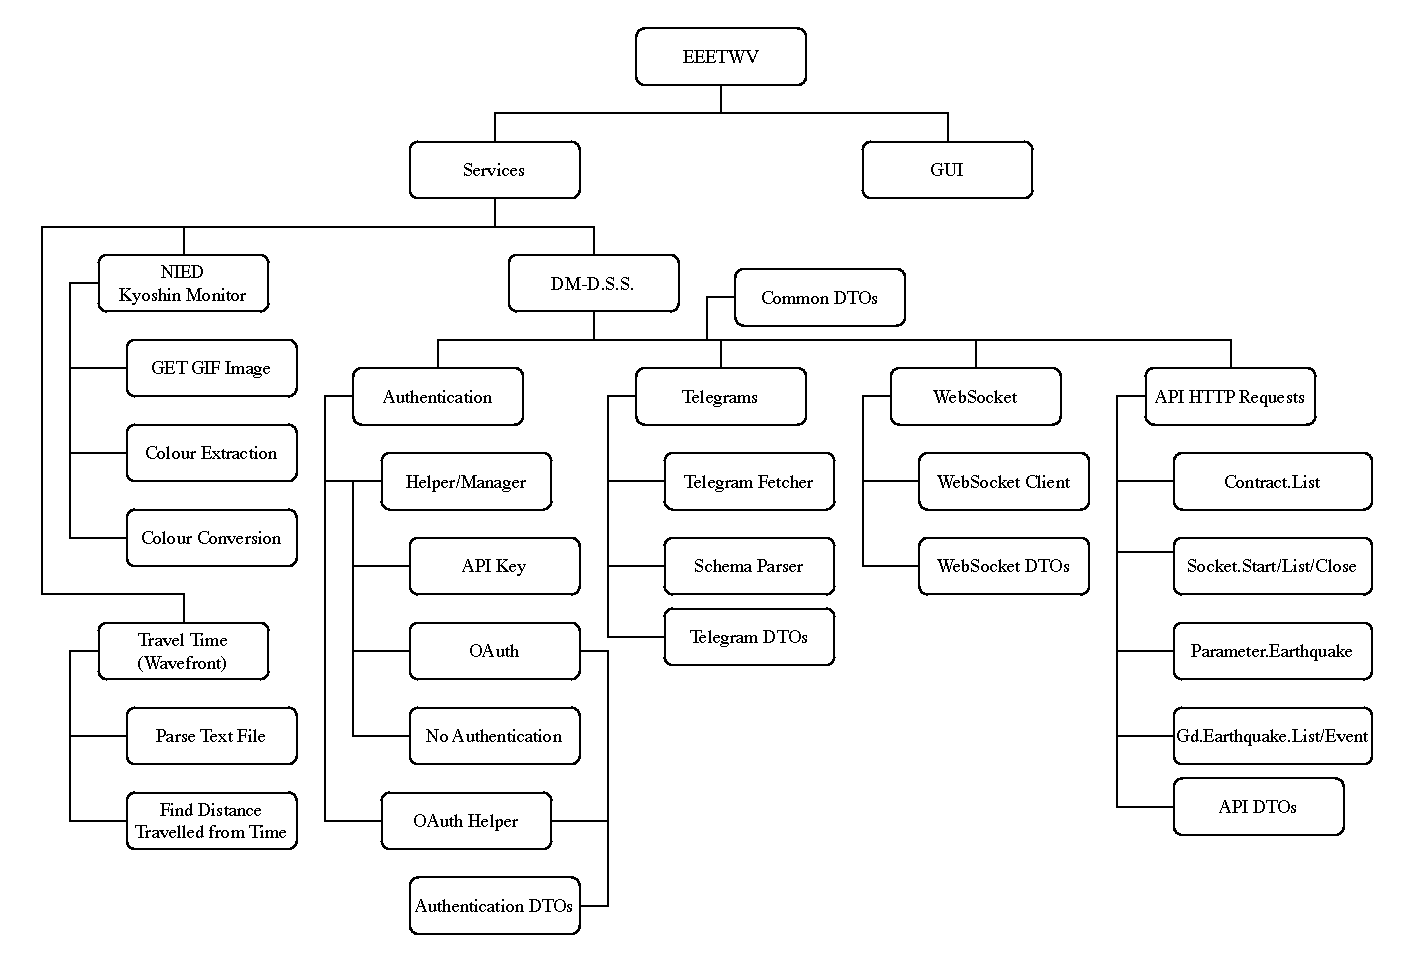
\includegraphics[width=\linewidth]{hierarchy.pdf}
    \caption{Hierarchy chart of the whole application}
    \label{fig:hierarchy}
\end{figure}

Since the GUI part is quite complicated, it is included in this separate diagram, in Figure \ref{fig:hierarchy-gui}.

\begin{figure}[htp]
    \centering
    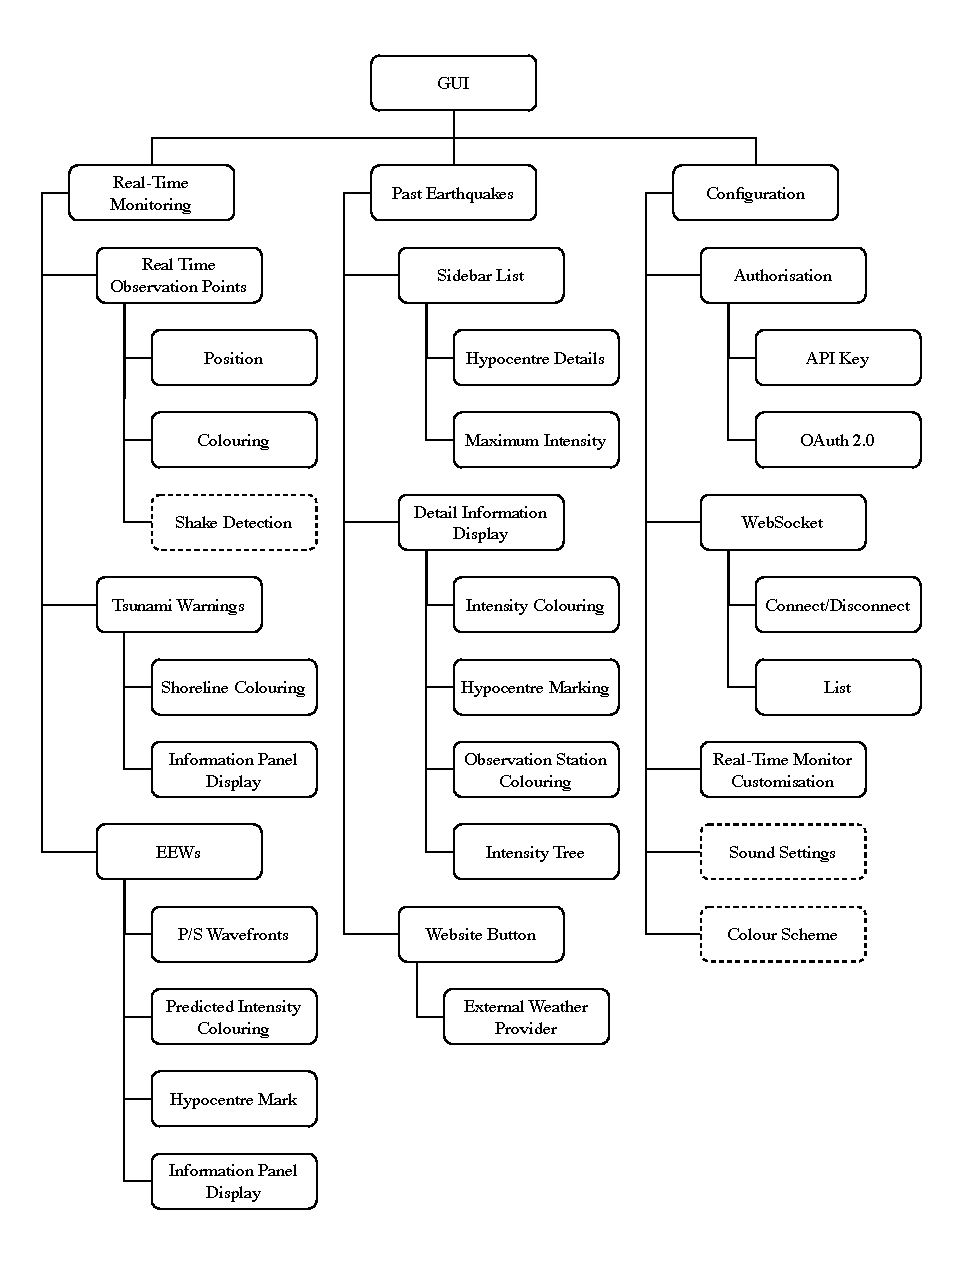
\includegraphics[width=0.8\linewidth]{hierarchy-gui.pdf}
    \caption{Hierarchy chart of the GUI Component}
    \label{fig:hierarchy-gui}
\end{figure}

The whole application (apart from the polynomial fitting part which was done in Python) will be written in C\# using the .NET Core Version 9.0, since the .NET Core is designed oriented around OOP techniques, and some JSON properties (e.g. the \Code{JsonStringEnumMemberName} to customise the parsing of enums) will require the use of .NET 9.

\section{External Data Sources}
There are two data sources this program will use: the NIED and the DM-D.S.S. Specifically, the former one is used to achieve the real-time shake data of the sensor points which were set up by the government (whose data is free to use), and the latter one is used to achieve past earthquake information and EEW information sent out by the JMA (which is pay-to-use). Note that DM-D.S.S. does also provide the real-time intensity data of the observation points, however it is pay-to-use only for companies and institutions on request. Therefore, it will not be feasible to use this data source in the program since one of and the principle target users is people passionate in monitoring earthquakes.

\subsection{NIED Data Source}

As mentioned before, NIED has numerous 'earthquake observation nets' across Japan. Specifically, there is the K-NET and KiK-net \autocite{nied-k-kik-net}, which is dedicated to the observation of strong seismic motion. The K-NET consists of approximately 1000 sensors located across Japan, while the KiK-net also includes some sensors which are located within the earth, which will often have different readings compared to those located on the surface. They are extremely capable of detecting strong motion of ground. Furthermore, the K-NET and the KiK-net provides real-time intensity data webpage of two types, the \href{http://www.kmoni.bosai.go.jp}{'Kyoshin' (強震) monitor} and the \href{https://www.lmoni.bosai.go.jp/monitor/}{long-period ground motion (LPGM, 長周期地震動) monitor} (not working at the time of investigation). The Hi-net \autocite{nied-hi-net} stands for high-sensitivity seismograph network, and it is dedicated for observation of minor motions of the ground. They release the waveforms to those who are researching seismic movements. As for the F-net \autocite{nied-f-net} which stands for the Full Range Seismograph Network of Japan, which is used to analyse the mechanism of a certain earthquake by analysing movements. None of the three nets provide a real-time API data feed.

Having compared the functionalities described above of the K/KiK-net, Hi-net and F-net and how they feed the data sources, the most suitable data source to reflect real-time motion of ground movements will be the \textbf{K/KiK-net}'s data feed, since it detects strong ground movements and is available real-time for the purpose of the application. (This is also the data source that JQuake and KEVI use in fact.)

In fact, in addition to these three networks, there are also the S-net, the DONET and the N-net, which detects the ground seismic movements in the sea. These data were adapted by SREV, but this is beyond the scope of this NEA analysis.

A comparison from the official website of MOWLAS (Monitoring of Waves on Land and Seafloor) \autocite{nied-mowlas} of the three nets are included in Figure \ref{fig:net-comparison} and a map of the distribution of the sensors are included in Figure \ref{fig:net-distribution}.

\begin{figure}[htp]
    \centering
    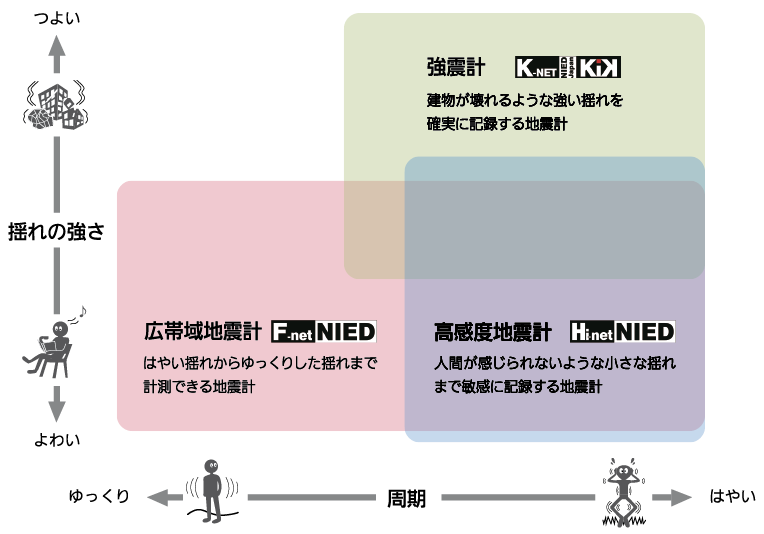
\includegraphics[width=0.75\linewidth]{net-comparison.png}
    \caption{A comparison of the K-NET, F-net and Hi-net}
    \label{fig:net-comparison}
\end{figure}

\begin{figure}[htp]
    \centering
    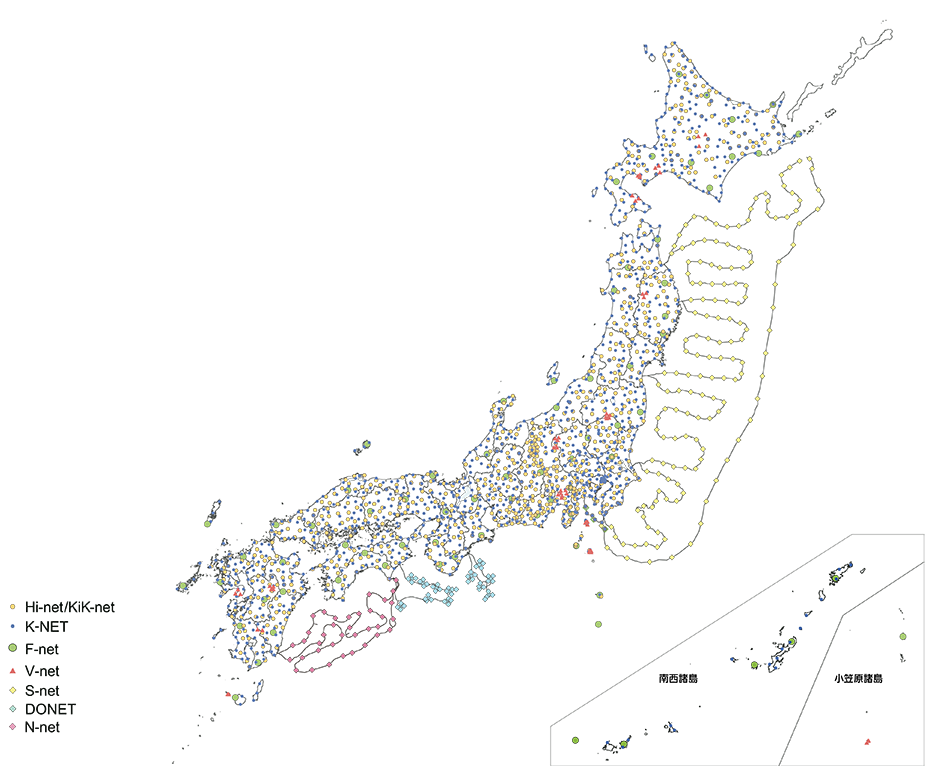
\includegraphics[width=0.75\linewidth]{net-distribution.png}
    \caption{Distribution of the sensors of different nets}
    \label{fig:net-distribution}
\end{figure}

\subsubsection{Achieving image format data source}

The data source fed by the 'Kyoshin' Monitor is split into 8 types (detailed below in Table \ref{tab:kmoni-data-types}), and each type split into 2 types of data sources, surface sensors and borehole (earth) sensors, with codes in Table \ref{tab:kmoni-sensor-types}. The link to the GIF image is in the following format:

\begin{center}
    \url{http://www.kmoni.bosai.go.jp/data/map_img/RealTimeImg/[#1]_[#2]/[yyyyMMdd]/[yyyyMMdd][hhmmss].[#1]_[#2].gif}
\end{center}

In the link, the \Code{[yyyyMMdd]} and the \Code{[hhmmss]} part should be replaced with the date and time respectively (in JST, UTC+8), and the \Code{#1} replaced with the codes detailed below for the data types, and \Code{#2} replaced with the codes detailed below for data sources. An example of the imaged achieved is in Figure \ref{fig:sample-kmoni}.

\begin{table}[htp]
    \centering

    \begin{tabular}{ccc}
        Data Type        & Description/Meaning                & Code in \Code{#1} \\
        \hline
        Real-time Shindo & Real-time Measured Intensity       & \Code{jma}        \\
        PGA              & Peak (Maximal) Ground Acceleration & \Code{acmap}      \\
        PGV              & Peak (Maximal) Ground Velocity     & \Code{vcmap}      \\
        PGD              & Peak (Maximal) Ground Displacement & \Code{dcmap}      \\
        Response 0.125Hz & Response spectrum for 0.125Hz PGV  & \Code{rsp0125}    \\
        Response 0.250Hz & Response spectrum for 0.250Hz PGV  & \Code{rsp0250}    \\
        Response 0.500Hz & Response spectrum for 0.500Hz PGV  & \Code{rsp0500}    \\
        Response 1.000Hz & Response spectrum for 1.000Hz PGV  & \Code{rsp1000}    \\
        Response 2.000Hz & Response spectrum for 2.000Hz PGV  & \Code{rsp2000}    \\
        Response 4.000Hz & Response spectrum for 4.000Hz PGV  & \Code{rsp4000}
    \end{tabular}
    \caption{Data available in 'Kyoshin' monitor}
    \label{tab:kmoni-data-types}
\end{table}

\begin{table}[htp]
    \centering

    \begin{tabular}{ccc}
        Sensor Type & Description/Meaning          & Code in \Code{#2} \\
        \hline
        Surface     & K-NET and KiK-net sensors    & \Code{s}          \\
        Borehole    & KiK-net sensors within earth & \Code{b}
    \end{tabular}
    \caption{Sensors available in 'Kyoshin' monitor}
    \label{tab:kmoni-sensor-types}
\end{table}

\begin{figure}[htp]
    \centering
    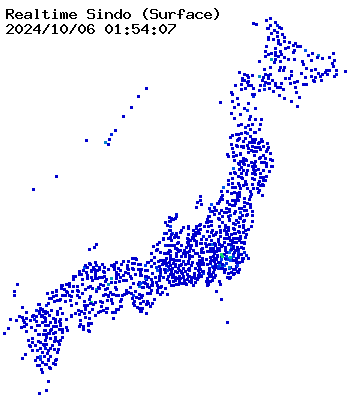
\includegraphics[width=0.5\linewidth]{sample-kmoni.png}
    \caption{Sample GIF image achieved from 'Kyoshin' Monitor}
    \label{fig:sample-kmoni}
\end{figure}

\subsubsection{Extracting colour for each observation point}

Unfortunately, it seems to the author (and is widely accepted in the EEW monitoring app development society) that the position of the points (squares) on the image does not follow any significant pattern of position, i.e. there is no obvious conversion of coordinates to us from the official longitude/latitude locations to the positions on the image. Therefore, a manual conversion one-to-one mapping has to be developed.

NIED does have an official released list of observation points, which include their names and positions. This list has around 1700 of those observation points. However, in the actual image (like those in Figure \ref{fig:sample-kmoni}), there are only 1000 of those in use in real time, consistent with K-NET's official introduction, and the rest 700 of those are invalid observation points. Therefore, it will be worth removing them from the list of earthquake monitoring points, before attempting to make the dictionary.

Unfortunately, 1000 is still quite a lot for us to deal with. Luckily, Ingen who used a similar approach to develop the KEVI application has already made such a mapping inside his open-source application in the file \href{https://github.com/ingen084/KyoshinEewViewerIngen/blob/develop/src/KyoshinEewViewer/Assets/ShindoObsPoints.mpk.lz4}{ShindoObsPoints.mpk.lz4} within \GitHubHref{ingen084}{KyoshinEewViewerIngen}, and even developed an editor for this at \GitHubHref{ingen084}{KyoshinShindoPlaceEditor}.

Due to the limited time for this NEA, the author will primarily use the pre-determined observation points for the K-NET and the KiK-net by Ingen in JSON format.

This paragraph referred to \autocite{blog-ingen-kmoni-data}.

\subsubsection{Converting colour to number format for further processing}

The true numerical data does not seem fully necessary at the first glance (since we might just as well just achieve the colour from the image and just plot them on the map, without the need to convert to a colour and back). However, for us to detect the shake in certain regions, it is necessary for us to achieve the numerical value to run the algorithm on it. Nevertheless, it is just good to have the number for us to have the numerical value for potential future developments.

\begin{figure}[htp]
    \centering
    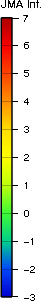
\includegraphics[scale = 0.6]{jma-scale.png}
    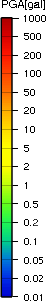
\includegraphics[scale = 0.6]{pga-scale.png}
    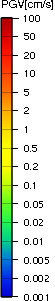
\includegraphics[scale = 0.6]{pgv-scale.png}
    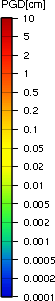
\includegraphics[scale = 0.6]{pgd-scale.png}
    \caption{Scale colours of different measurements}
    \label{fig:scale-colour}
\end{figure}

As shown in Figure \ref{fig:scale-colour}, the NIED 'Kyoshin' Monitor does indeed provide a scale of colours and reference to numerical values. However, there is a chance that a certain colour is not 'exactly' mapped on the scale, and further concerning that it is very slow and difficult to 'loop over' a colour legend, it is necessary to have an algorithmic-approach (numerical mapping-based approach) to map the colours in the colour space to numerical values (and back) is necessary.

\paragraph{Abstraction of colour scale}

Notice that the scale for PGA/PGV/PGD follow a logarithmic scale, while measured intensity follows a linear scale (though noting that the way intensity and magnitude is calculated is logarithmic as well). Therefore, if we normalise the vertical distance from the bottom of the axis \(h\) to \(0 \leq h \leq 1\) (i.e. \(h = 0\) at the bottom of the scale, \(h = 1\) at the top of the scale), and if we denote intensity using \(I\) in JMA scale, PGA as \(a\) in gal, PGV as \(v\) in cm per second, and PGD as \(s\) in cm, from the scale, the following transforming formulae obviously hold:
\begin{align*}
    I  = 10h - 3     & \iff h      = \frac{I + 3}{10}, \\
    a  = 10^{5h - 2} & \iff h  = \frac{\lg a + 2}{5},  \\
    v  = 10^{5h - 3} & \iff h  = \frac{\lg v + 3}{5},  \\
    x  = 10^{5h - 4} & \iff h  = \frac{\lg x + 4}{5}.  \\
\end{align*}

However, it is worth noting that NIED did use \(1, 2, 5, 10\) on the logarithmic scale at equal intervals, so it is not a perfect logarithmic scale. The author is unsure why they designed the scale like this, nor if it's an intended approximation. Nevertheless, the logarithmic scale is a good enough approximation.

The next step is to develop a mapping from this colour space \(\mathcal{C}\) to \(h\), which of course should be invertible. Denote this as \(f: [0, 1] \to \mathcal{C}\).

\paragraph{Describing colour numerically}

We consider using a suitable base to decompose \(\mathcal{C}\). The colour of the given scale is an immediate suggestion to use a base containing \textbf{hue}, which in fact is designed to describe how human perceive colour, and unlike RGB and CMYK which uses principle colours to describe colour. A hue scale is shown in Figure \ref{fig:hue-scale}.

\begin{figure}[htp]
    \centering
    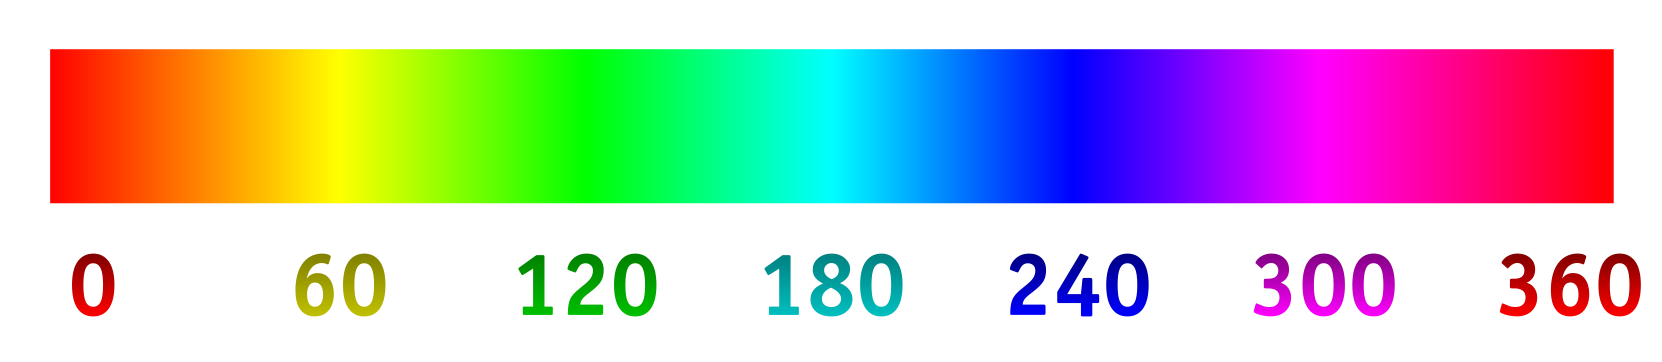
\includegraphics[scale = 0.15]{hue-scale.png}
    \caption{The hue scale in HSL/HSV encoding}
    \label{fig:hue-scale}
\end{figure}

Therefore, a colour in the colour space \(\mathcal{C}\) can be represented as a 3-D vector \(\mathcal{C} \ni C = (H, S, V)\), where \(H \in [0, 360)\) in degrees is the hue value, \(S \in [0, 1]\) stands for the saturation, and \(V \in [0, 1]\) stands for the value (a brightness). And hence we will be able to decompose \(f\) into three components \(f = \left(f_H, f_S, f_V\right)\).

Figure \ref{fig:hsv-against-row} plots the values of \(H, S\) and \(V\) against \(h\) (this is the graph of \(f\) and its components) of discrete values of \(h\), and depending on the result we will attempt some fit/regression to a suitable function.

\begin{figure}[htp]
    \centering
    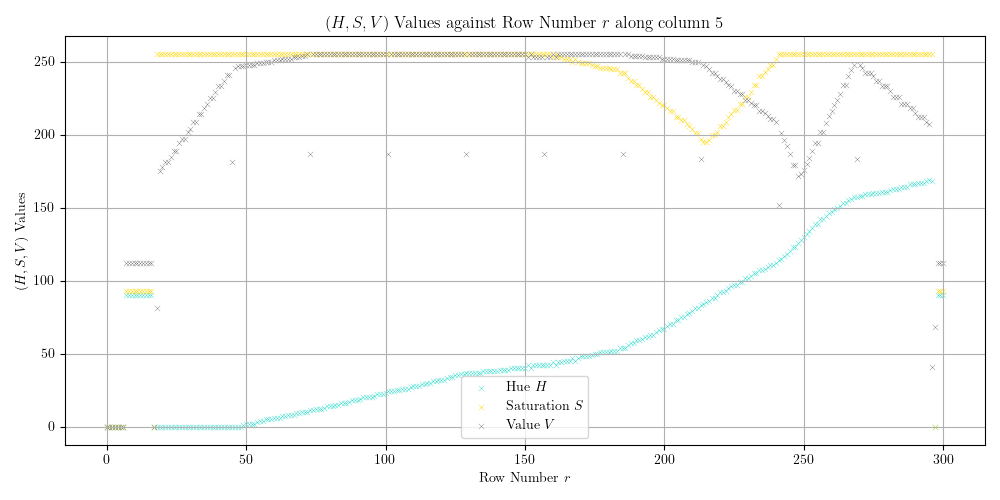
\includegraphics[scale = 0.60]{hsv-against-row.png}
    \caption{The values of \((H, S, V)\) against pixel row \(r\)}
    \label{fig:hsv-against-row}
\end{figure}

Notice that in this plot, all values of \((H, S, V)\) in fact range from \(0\) to \(255\), as in an 8-bit binary.

It is worth noting that the scale has some space on the top (to show the type), and some space at the bottom. Notice that when the row \(r = 17\) and \(r = 297\) have values significantly different, so we extract the rows \(r = 18\) and \(r = 296\) to correspond (linearly) to \(h = 1\) and \(h = 0\), i.e.,
\[
    h = 1 - \frac{r - 18}{278}.
\]

Figure \ref{fig:hsv-against-h} shows the result of this transformation being applied.

\begin{figure}[htp]
    \centering
    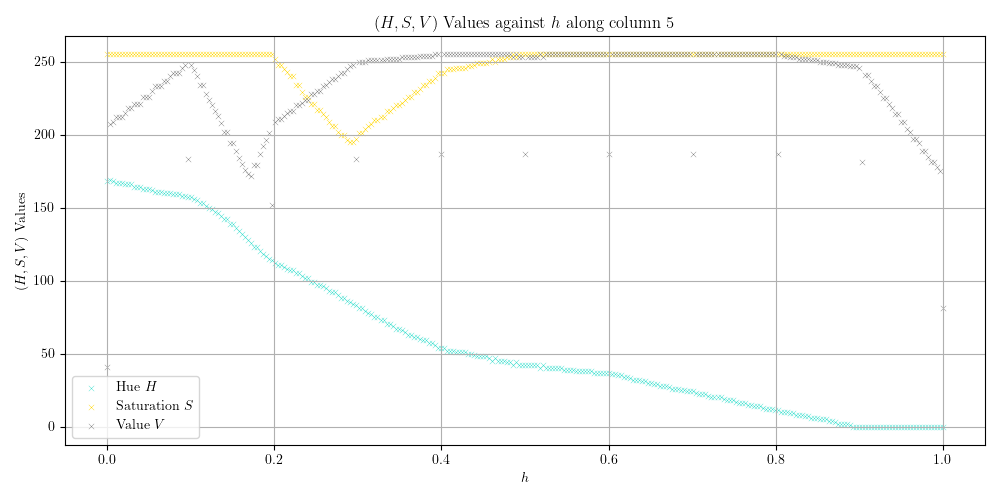
\includegraphics[scale = 0.60]{hsv-against-h.png}
    \caption{The values of \((H, S, V)\) against normalised height \(h\)}
    \label{fig:hsv-against-h}
\end{figure}

From here onwards, all values of \((H, S, V)\) will be adjusted to be within the range which they should be in, i.e. \(H \in [0, 360), S \in [0, 1], V \in [0, 1]\).

\paragraph{Finding \(f_H\) in terms of \(h\)}

We consider finding \(f_H\) first, which is the cyan line. Notice that its trend can be split into 4 parts:
\begin{itemize}
    \item \(h \in [0, 0.1]\): linear;
    \item \(h \in [0.1, 0.6]\): curving, ideally a cubic;
    \item \(h \in [0.6, 0.9]\): linear;
    \item \(h \in [0.9, 1]\): constant (0).
\end{itemize}

\begin{table}[htp]
    \centering

    \begin{tabular}{|c|c|}
        \hline
        \(h\) & \(H = f_H(h)\) \\
        \hline
        0     & 237            \\
        0.1   & 222            \\
        0.6   & 51             \\
        0.9   & 0              \\
        1     & 0              \\
        \hline
    \end{tabular}
    \caption{Initial values for \(f_H\)}
    \label{tab:h-against-h-iv}
\end{table}

Furthermore, boundary conditions in Table \ref{tab:h-against-h-iv} are applied to ensure that the function is continuous and nicely-behaving while matching the existing data. We use the following function to apply the fit:
\[
    f_H(h) = \begin{cases}
        -150h + 237, & h \in [0, 0.1],   \\
        \odot,       & h \in [0.1, 0.6], \\
        -170h + 153, & h \in [0.6, 0.9], \\
        0,           & h \in [0.9, 1].
    \end{cases}
\]

Here,
\begin{align*}
    \odot & = \frac{222 \cdot (h - 0.3) \cdot (h - 0.4) \cdot (h - 0.6)}{(0.1 - 0.3) \cdot (0.1 - 0.4) \cdot (0.1 - 0.6)} \\
          & + \frac{y_1 \cdot (h - 0.1) \cdot (h - 0.4) \cdot (h - 0.6)}{(0.3 - 0.1) \cdot (0.3 - 0.4) \cdot (0.3 - 0.6)} \\
          & + \frac{y_2 \cdot (h - 0.1) \cdot (h - 0.3) \cdot (h - 0.6)}{(0.4 - 0.1) \cdot (0.4 - 0.3) \cdot (0.4 - 0.6)} \\
          & + \frac{51 \cdot (h - 0.1) \cdot (h - 0.3) \cdot (h - 0.4)}{(0.6 - 0.1) \cdot (0.6 - 0.3) \cdot (0.6 - 0.4)}.
\end{align*}

Here, \(m_1\) is the gradient of the line for \(h \in [0, 0.1]\), \(y_1 = f_H(0.3), y_2 = f_H(0.4)\) for \(h \in [0.1, 0.6]\) (using Lagrange Polynomial), and the equation between \(h \in [0.6, 0.9]\) is in fact fixed due to the initial conditions.

By applying a curve fit to the original data, the following results are obtained:
\[
    (y_1, y_2) = (115, 79.5).
\]

Plotting \(H\) and \(f_H(h)\) against \(h\) gives us Figure \ref{fig:h-against-h}, which is decent.

\begin{figure}[htp]
    \centering
    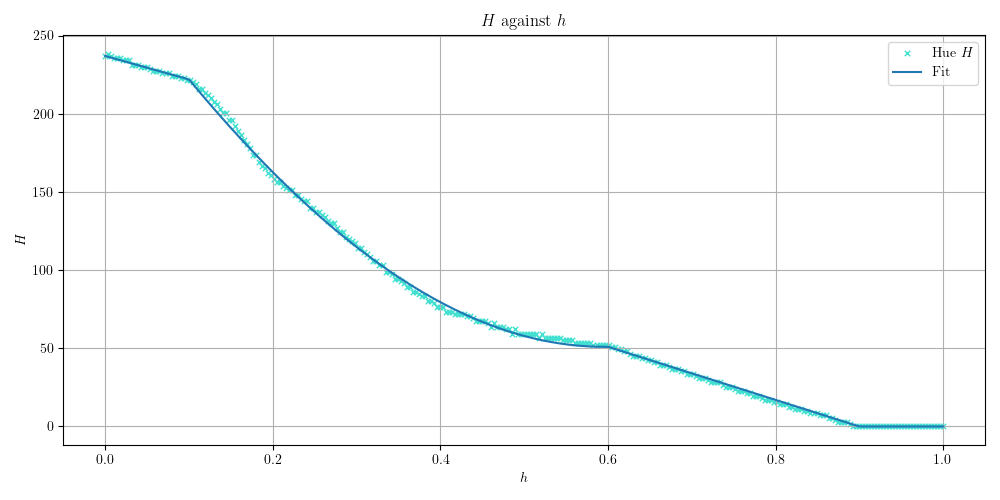
\includegraphics[scale = 0.60]{h-against-h.png}
    \caption{The fit result for \(f_H: h \mapsto H\)}
    \label{fig:h-against-h}
\end{figure}

\paragraph{Finding \(f_S\) in terms of \(h\)}

As for \(f_S(h)\), the obvious thing to do is to split it into 5 (4) piecewise functions, specifically \(f_S = 1\) for \(h \in [0, 0.2] \cup [0.5, 1]\), and three linear functions for \(h \in [0.2, 0.29], h \in [0.29, 0.4]\) and \(h \in [0.4, 0.5]\). Initial values are included in Table \ref{tab:s-against-h-iv}.

\begin{table}[htp]
    \centering

    \begin{tabular}{|c|c|}
        \hline
        \(h\) & \(S = f_S(h)\) \\
        \hline
        0     & 1              \\
        0.2   & 1              \\
        0.29  & 0.765          \\
        0.4   & 0.95           \\
        0.5   & 1              \\
        1     & 1              \\
        \hline
    \end{tabular}
    \caption{Initial values for \(f_S\)}
    \label{tab:s-against-h-iv}
\end{table}

This gives us that
\[
    f_S(h) = \begin{cases}
        1,              & h \in [0, 0.2],    \\
        -2.611h + 1.522 & h \in [0.2, 0.29], \\
        1.682h + 0.277, & h \in [0.29, 0.4], \\
        0.5h + 0.75     & h \in [0.4, 0.5],  \\
        1,              & h \in [0.5, 1].
    \end{cases}
\]

Plotting this out gives Figure \ref{fig:s-against-h}.

\begin{figure}[htp]
    \centering
    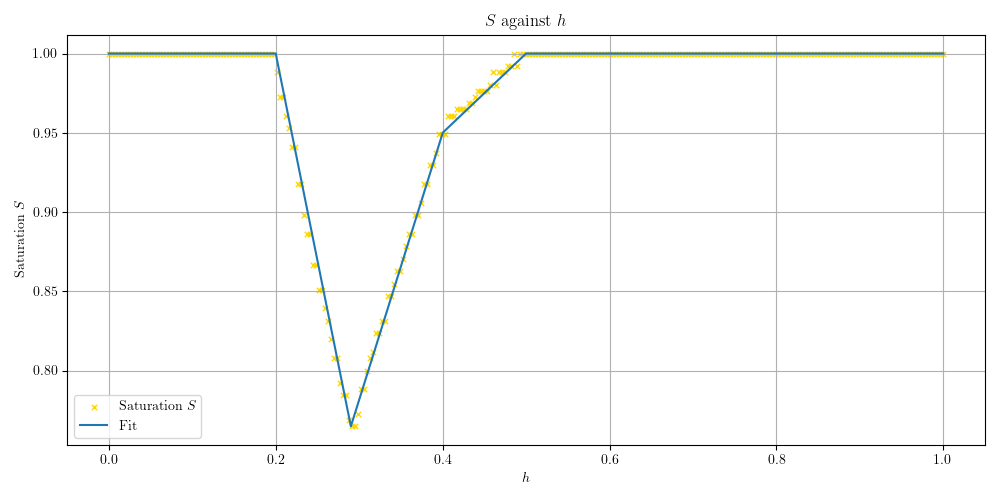
\includegraphics[scale = 0.60]{s-against-h.png}
    \caption{The fit result for \(f_S: h \mapsto S\)}
    \label{fig:s-against-h}
\end{figure}

\paragraph{Finding \(f_V\) in terms of \(h\)}

As for \(f_V(h)\), we shall divide it into even more piecewise linear functions. Specifically, I chose to divide the interval \([0, 1]\) at \(0.1, 0.172, 0.2, 0.3, 0.4, 0.8\) and \(0.9\). Initial values are included in Table \ref{tab:v-against-h-iv}.

\begin{table}[htp]
    \centering

    \begin{tabular}{|c|c|}
        \hline
        \(h\) & \(V = f_V(h)\) \\
        \hline
        0     & 0.8            \\
        0.1   & 0.98           \\
        0.172 & 0.66           \\
        0.2   & 0.82           \\
        0.3   & 0.98           \\
        0.4   & 1              \\
        0.8   & 1              \\
        0.9   & 0.97           \\
        1     & 0.68           \\
        \hline
    \end{tabular}
    \caption{Initial values for \(f_V\)}
    \label{tab:v-against-h-iv}
\end{table}

This gives us the piecewise function
\[
    f_V(h) = \begin{cases}
        1.8h + 0.8,      & h \in [0, 0.1],     \\
        -4.444h + 1.424, & h \in [0.1, 0.172], \\
        5.714h - 0.323,  & h \in [0.172, 0.2], \\
        1.6h + 0.5,      & h \in [0.2, 0.3],   \\
        0.2h + 0.92,     & h \in [0.3, 0.4],   \\
        1,               & h \in [0.4, 0.8],   \\
        -0.3h + 1.24,    & h \in [0.8, 0.9],   \\
        -2.9h + 3.58,    & h \in [0.9, 1].
    \end{cases}
\]

Plotting this out gives us Figure \ref{fig:v-against-h}.

\begin{figure}[htp]
    \centering
    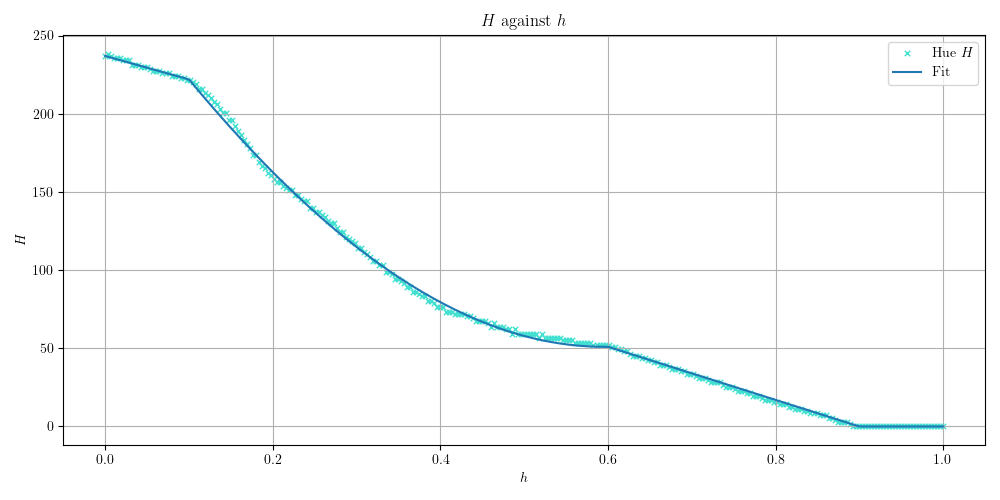
\includegraphics[scale = 0.60]{v-against-h.png}
    \caption{The fit result for \(f_V: h \mapsto V\)}
    \label{fig:v-against-h}
\end{figure}

Note that in this plot, \(V\) when \(h = 0\) or \(h = 1\) is excluded, since just like every \(h = 0.1 k\) for some \(k \in \mathbb{N}\), they are anomalies created by the horizontal black line in the scale.

\paragraph{Finding \(f^{-1}\)}

To find \(f^{-1}: \mathcal{C} \to [0, 1]\), we do not need necessarily to find an expression of \(h\) in terms of \((H, V, S)\). If we notice that \(f_H\) is one-to-one on \(h \in [0, 0.9]\), and \(f_V\) is one-to-one on \(h \in [0.9, 1]\), we can use \(f_H^{-1}\) to determine \(h\) from \(H\) only if \(H\) is non-zero, and use \(f_V^{-1}\) otherwise.

\[
    f^{-1}(H, S, V) = \begin{cases}
        f_H^{-1}(H), & H \neq 0, \\
        f_V^{-1}(V), & H = 0.
    \end{cases}
\]

Notice that for \(h \in [0.1, 0.6]\), \(f_H\) is a cubic and is not easily invertible. However, it would be plausible to use a binary-search algorithm to find \(h\) based on \(H\) since it is monotonic, and it is within a reasonable amount of time, to relatively good precision. Otherwise, on the linear parts, it is fine to simply mathematically invert it.

Algorithm \ref{alg:cap} describes the logic. Note that, this algorithm uses different \(V\) ranges from before (which is consistent with SkiaSharp library in C\#), and the ranges is \(V \in [0, 100]\). Notice that, \(\epsilon(h)n\) and \(\epsilon(H)\) are two constant values that determines the precision of such binary search, and they are chosen to be \(0.01\) and \(0.5\) in the implementation.

\begin{algorithm}[htp]
    \caption{Algorithm for \(f^{-1}\)}\label{alg:cap}
    \begin{algorithmic}
        \Require \(H \in [0, 360)\)
        \Require \(S \in [0, 100]\)
        \Require \(V \in [0, 100]\)
        \Ensure \(h \in [0, 1]\)
        \State \(V \gets V / 100\) \Comment{Normalise \(V\)}
        \If{\(V\) is \(0\)} \Comment{Use \(V\)}
        \State \Return \((V - 3.50) / (-2.9)\)
        \Else \Comment{Use \(H\)}
        \LComment{Deal with out-of-range \(H\)s, and use inverse linear functions}
        \If{\(H \geq 222\)}
        \State \Return \((H - 237) / (-150)\)
        \ElsIf{\(H \leq 51\)}
        \State \Return \((H - 153) / (-170)\)
        \LComment{Inverse-Cubic by Binary Search, with set errors}
        \Else
        \State \(l \gets 0.1\)
        \State \(r \gets 0.6\)
        \LComment{Checks if the normalised height is already precise enough}
        \While{\(r - l \geq \epsilon(h)\)}
        \State \(m \gets (l + r) / 2\)
        \State \(c \gets \Call{Height to Hue}{m}\)
        \LComment{Checks if the calculated hue is already precise enough}
        \If{\(\left\lvert c - H\right\rvert \leq \epsilon(H)\)}
        \State \Return \(m\)
        \ElsIf{\(c > H\)}
        \State \(l \gets m\)
        \ElsIf{\(c < H\)}
        \State \(r \gets m\)
        \EndIf
        \EndWhile

        \State \Return \((l + r) / 2\)
        \EndIf
        \EndIf
    \end{algorithmic}
\end{algorithm}

\subsubsection{Flowchart of data and sidenotes}

To summarise, we discussed the mapping from the colour space\(\mathcal{C}\) to the normalised height \(h\), and back, and we also discussed how \(h\) is related with the measured intensity \(I\), the PGA \(a\), the PGV \(v\), and the PGD \(x\). They can be transformed forwards and backwards using simple mathematical explicit relations, and specifically for \(f_H^{-1}(H)\) will use a binary search algorithm.

Figure \ref{fig:kmoni-data-flow} shows the data flow, Figure \ref{fig:variable-relation} shows the relation between abstract variables, and \ref{fig:generated-colour} shows the result of colour generated compared with the original.

\begin{figure}[htp]
    \centering
    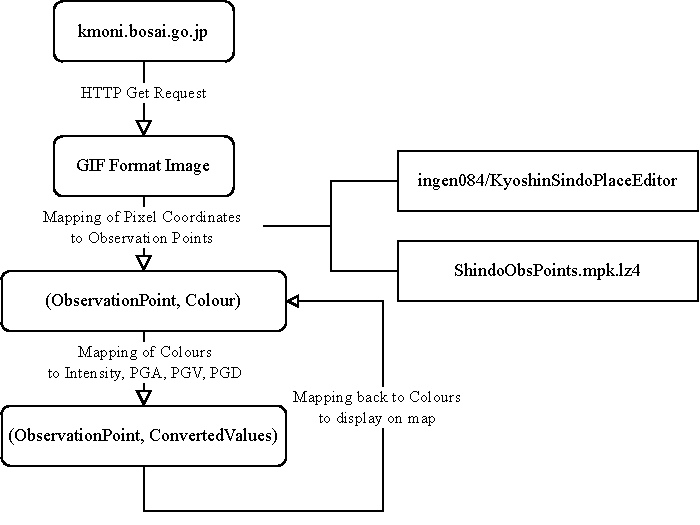
\includegraphics[width=0.8\linewidth]{kmoni-data-flow.pdf}
    \caption{Flow of data in NIED data sources}
    \label{fig:kmoni-data-flow}
\end{figure}

\begin{figure}[htp]
    \centering
    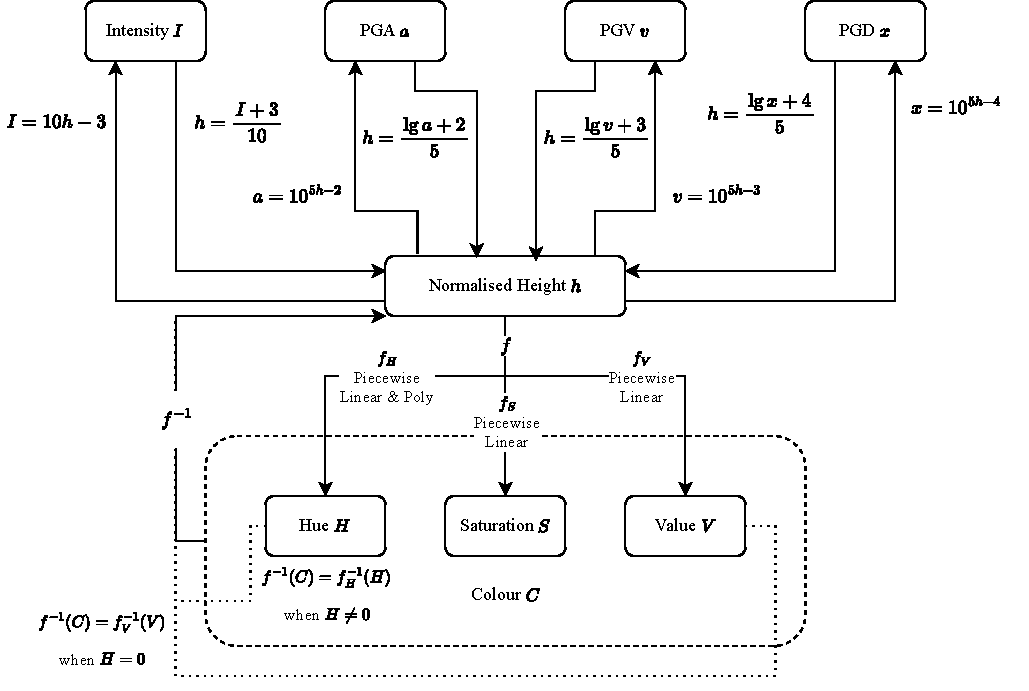
\includegraphics[width=0.9\linewidth]{variable-relation.pdf}
    \caption{Relation between abstract variables}
    \label{fig:variable-relation}
\end{figure}

\begin{figure}[htp]
    \centering
    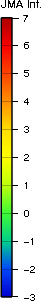
\includegraphics[scale = 0.6]{jma-scale.png}
    
\includegraphics[scale = 0.6]{generated-colour.png}
    \caption{Colour generated using fitted functions}
    \label{fig:generated-colour}
\end{figure}

It is worth noting that an existing NuGet Library, \GitHubHref{ingen084}{KyoshinMonitorLib} and introduced in \autocite{blog-ingen-kmoni-nuget-lib} which is designated to manage intensities, as well as extracting intensities from the 'Kyoshin' monitor. This NEA did refer to this for some guidance but is not dependent on this library, and its necessary functionalities within the scope of this NEA is realised again using the author's own code. The developer of this library did also mention that it is quite purpose-built so might not be suitable for general use.

It is also worth noting that, technically, scraping the data from the 'Kyoshin' monitor page of NIED is not explicitly allowed, but not explicitly banned either. However, extracting and displaying numerical data in the application is strictly banned by the NIED, and therefore the numerical values will only serve as internal values of the application and will not be displayed to the users in any way.

This paragraph referred to \autocite{blog-jquake-poly-fit}. The code used for this section is in Listing \ref{code-listing:poly-fit}.

\subsection{DM-D.S.S. Data Source}

DM-D.S.S. is a well-structured official data source with low latency and reliable information and services. This is going to be the primary data source for most part of the application.

Their APIs are split into two types: HTTP based requests and WebSocket based connections. HTTP based requests are typically for more static information, while WebSocket connections are for live time-essential data feeds, such as the EEW warnings, tsunami warnings and latest earthquake information.

\subsubsection{Authorisation}

There are two types of authorisation that DM-D.S.S. supports, API Keys and OAuth2 Access Tokens.

API Keys access tokens are extremely easy to program, since it simply uses Basic Authorisation in the header, and uses the key as the username (without a password). It uses the Basic BasicBase64 Authorisation encoding. However, this introduces an extra layer of complexity for the users, since they would have to go to the settings of the DM-D.S.S. webpage and achieve an API Key to paste into the application, as shown in Figure \ref{fig:api-key-control-panel}.

\begin{figure}[htp]
    \centering
    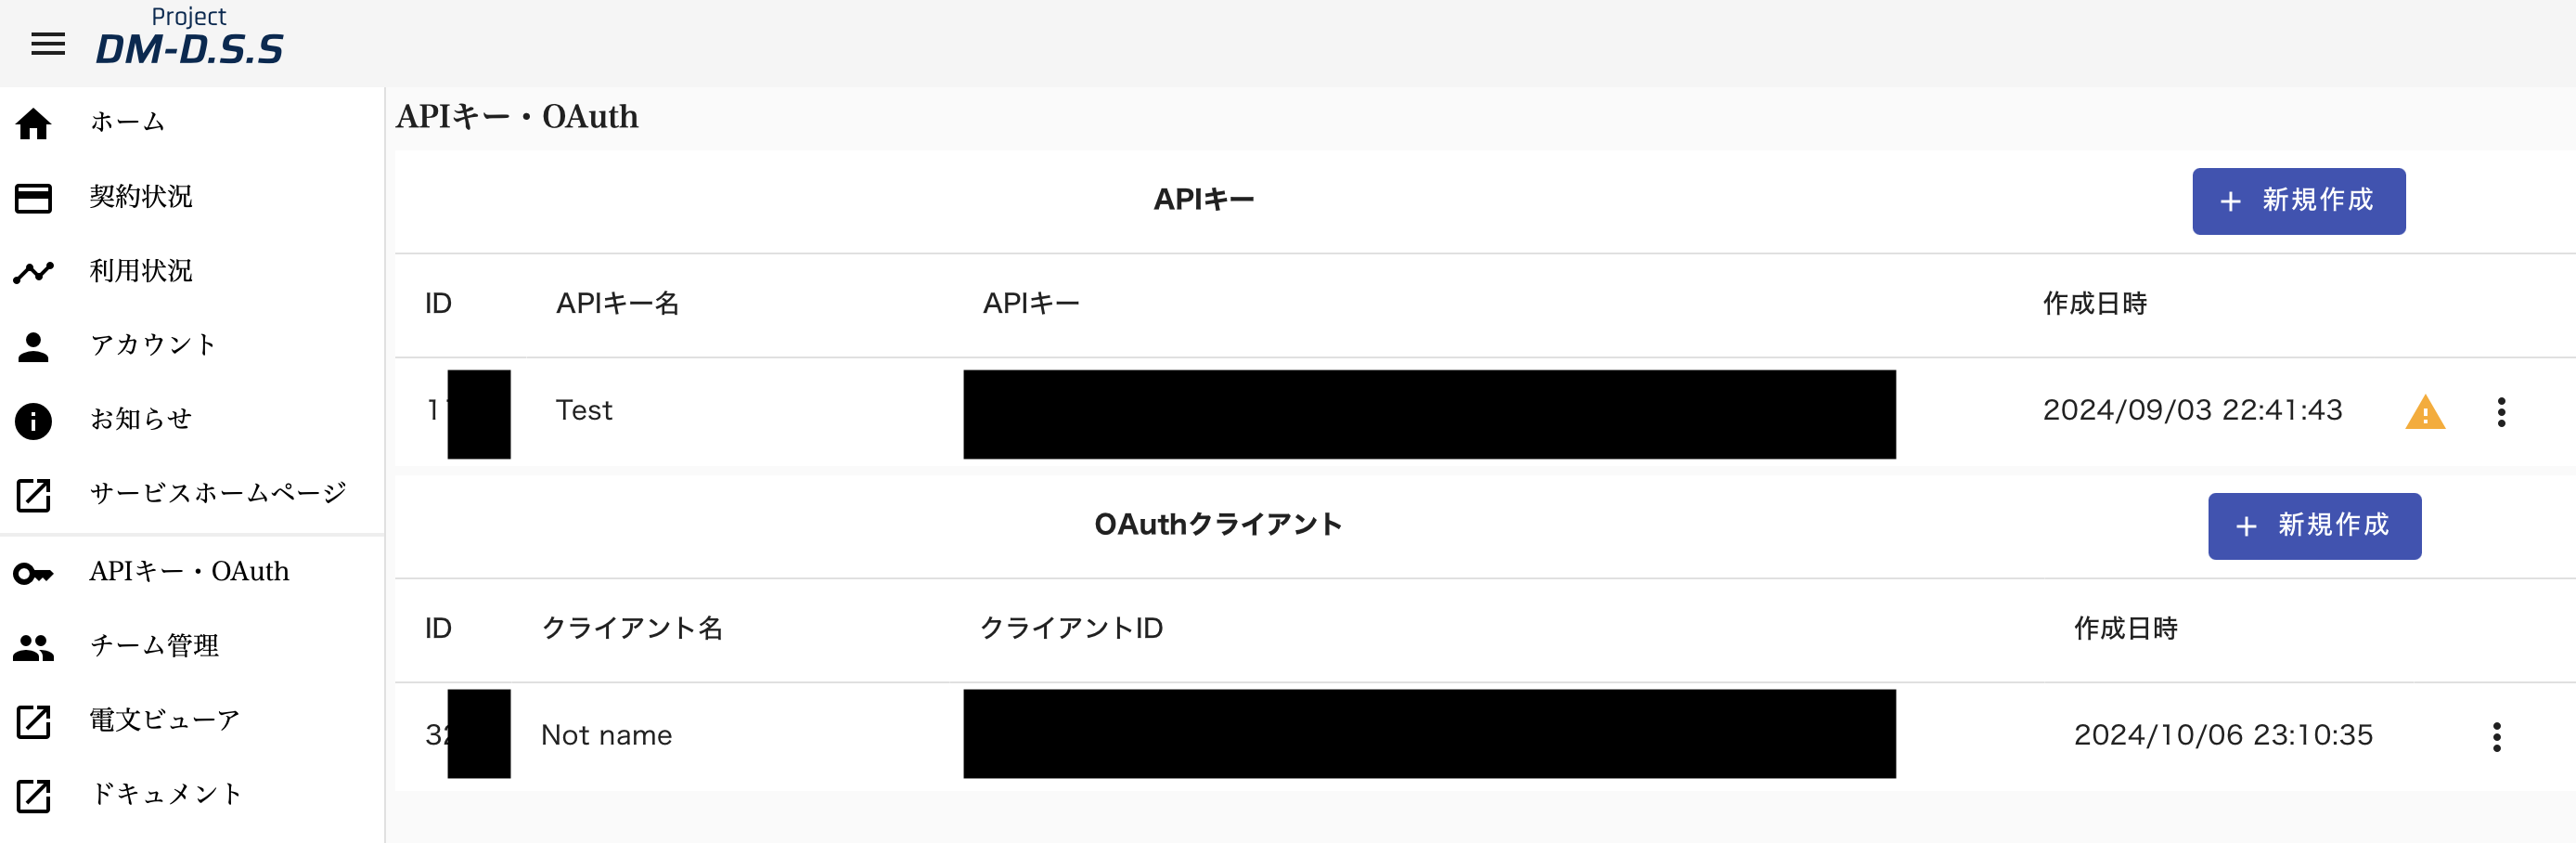
\includegraphics[width=0.7\linewidth]{api-key-control-panel.png}
    \caption{Control panel for API Keys}
    \label{fig:api-key-control-panel}
\end{figure}

As for OAuth2, it will be much simpler for the users, since it will provide the user with a login interface on the website, and ask them to give the program certain permissions, which is just a few simple clicks. Rather than using the user as a bridge for sharing the credentials with the application, they are shared between the authorisation server (DM-D.S.S.) and the application directly, without the need for the user to deal with such human-unreadable codes.

\paragraph{OAuth 2.0}

OAuth 2.0 is a standard protocol that allows a user to authorise an application without sharing any of their credentials. Figure \ref{fig:oauth-outline} gives a brief outline of the procedure involved.

\begin{figure}[htp]
    \centering
    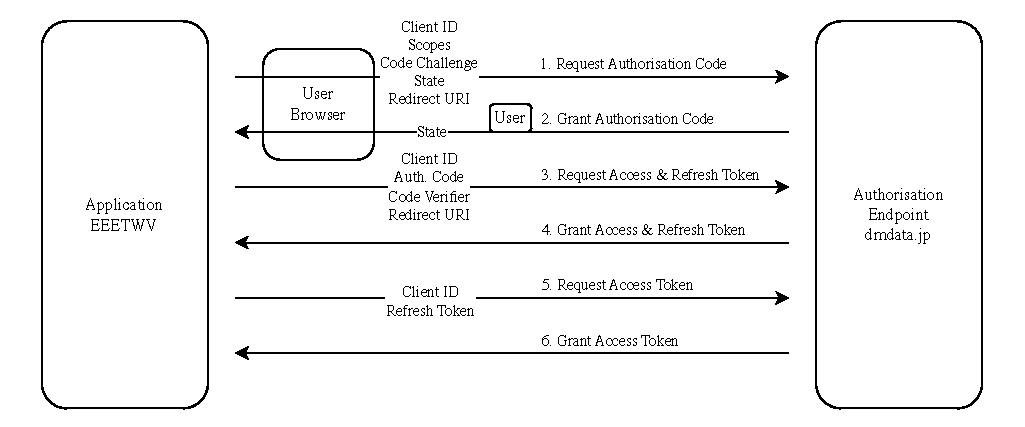
\includegraphics[width=\linewidth]{oauth-outline.pdf}
    \caption{OAuth Procedure Outline}
    \label{fig:oauth-outline}
\end{figure}

\subparagraph{Authorisation Code}

The authorisation begins with the application requesting an \textbf{authorisation token} from the authorisation endpoint, via the user's browser. This is the only step where the user has to be involved, but all they have to do is log-in to their DM-D.S.S. account and click the 'grant' button on the page.

First, the user launches the browser to the authorisation endpoint (Step 1)
\begin{center}
    \url{https://manager.dmdata.jp/account/oauth2/v1/auth}
\end{center}
with the following parameters:
\begin{itemize}
    \item \Code{client_id}: the client ID for the application to grant (which is public and safe to be seen by the user);
    \item \Code{redirect_uri}: redirect URL for the endpoint to redirect to, to inform the application of the authorisation results;
    \item \Code{response_type}: \Code{code}
    \item \Code{response_mode}: the way to response to the application (we will only use the response type \Code{query});
    \item \Code{scope}: the string containing the permissions the application is requesting, separated by a space;
    \item \Code{state}: the state which will be returned by the return query to prevent CSRF attacks;
    \item \Code{code_challenge}: the code challenge for PKCE;
    \item \Code{code_challenge_method}: the way to encode the code challenge (we will use \Code{S256}).
\end{itemize}

At the same time as launching the browser, the program should start a listener on the local IP address and port specified in the redirect URL, and wait until it receives a request from the browser. In the response (Step 2), it will contain two parameters: \Code{code} which contains the authorisation code (which is only valid for 10 minutes), and \Code{state} which should be the same as the state sent in the request.

The reason why the \textbf{state} is essential is to prevent CSRF (Cross-Site Request Forgery) attacks, where the application can make sure the response is truly corresponding to the request the application made (not by any other applications), and no one forged a response to the application (pretended to be the browser acting as authorisation endpoint). Verifying the state is essential for the security of the application.

If the request fails, the return query will return the \Code{error}, and with the \Code{state} as well. Table \ref{tab:oauth2-auth-code-errors} includes a table of errors that could occur in the authorisation code request.

\begin{table}
    \centering
    \begin{tabular}{cc}
        Error Code                               & Description                                            \\
        \hline
        \Code{invalid_request}                   & The parameters are invalid.                            \\
        \Code{invalid_client}                    & The Client ID is invalid.                              \\
        \Code{invalid_redirect_url}              & The redirect URL is not supported by the Client ID.    \\
        \Code{invalid_scope}                     & The scope string is invalid.                           \\
        \Code{unauthorized_client}               & The client to authorise using this method is invalid.  \\
        \Code{access_denied}                     & The access is denied.                                  \\
        \Code{recaptcha_verification_failed}     & The reCAPTCHA verification failed.                     \\
        \Code{unsupported_response_type}         & The response type is not recognised.                   \\
        \Code{unsupported_code_challenge_method} & The code challenge method is not recognised.           \\
        \Code{no_signin}                         & The user is not signed in (usually should not happen). \\
        \Code{server_error}                      & The internal server encountered an error.
    \end{tabular}
    \caption{Error codes for authorisation code step in OAuth2}
    \label{tab:oauth2-auth-code-errors}
\end{table}

In the application, only the errors \Code{access_denied}, \Code{recaptcha_verification_failed}, \Code{no_signin} and \Code{server_error} should appear (and the final two shouldn't appear usually), since all other errors are due to issue with design of the application.

\subparagraph{Refresh and Access Token}

After this step, the program will use the authorisation token to request an \textbf{access token} which comes with a \textbf{request token} (Step 3). The program will send an HTTP POST request to the token endpoint
\begin{center}
    \url{https://manager.dmdata.jp/account/oauth2/v1/token}
\end{center}
with the following query parameters, in URL Encoded form:
\begin{itemize}
    \item \Code{client_id}: the client ID for the application to grant (which is public and safe to be seen by the user);
    \item \Code{grant_type}: \Code{authorization_code};
    \item \Code{code}: the authorisation code received from the previous step;
    \item \Code{redirect_uri}: the redirect URL used in the previous step;
    \item \Code{code_verifier}: the original version of the code challenge used in the previous step.
\end{itemize}

Now the reason of the code challenge and code verifier is apparent (they are part of PKCE, Proof Key for Code Exchange): since the code challenge is a hashed version of the code verifier and is exchanged in the first step, the code verifier (the plain version) is used to prove that the application is the same as the one that requested the authorisation code. This means, if a man-in-the-middle acquired the authorisation code and the code challenge, they would not be able to use it, since it requires them to reverse hash the code challenge to get the code verifier, which is impossible in a reasonable amount of time. To ensure the security, the code verifier should be generated randomly and be very long, and disposed after each use.

The response (Step 4) will be JSON format, as shown in Listing \ref{code:oauth-access-token-request}.

\begin{listing}[htp]
    \inputminted{json}{code/OAuthAccessTokenRequest.json}
    \caption{Response for OAuth Access Token Request}
    \label{code:oauth-access-token-request}
\end{listing}

The properties \Code{token_type}, and \Code{expires_in} are constants, the \Code{scope} are the scopes which are authorised for, and the most important two are the \Code{access_token} and \Code{refresh_token}.

The refresh token is a long-living token, and it has lifetime 183 days in DM-D.S.S., resetting every time a new access token is acquired (see below). On the other hand, the access token is a short-living token, and it has lifetime 6 hours only. This does not mean that the access token should be disposed per-use -- it should be reused within the application, and only when it expires, a new access token should be requested using the refresh token. However, when the application is closed, only the refresh token should be stored, and the access token revoked -- next time the application launches, the access token should be acquired again.

If the request failed, then an error will be returned, also in JSON format, as shown in Listing \ref{code:oauth-error}.

\begin{listing}[htp]
    \inputminted{json}{code/OAuthError.json}
    \caption{Error for OAuth Access Token Request}
    \label{code:oauth-error}
\end{listing}

Table \ref{tab:oauth2-access-token-errors} includes a table of errors that could occur in the authorisation code request.

\begin{table}
    \centering
    \begin{tabular}{cc}
        Error Code                    & Description                                           \\
        \hline
        \Code{invalid_request}        & The parameters are invalid.                           \\
        \Code{invalid_client}         & The Client ID is invalid.                             \\
        \Code{invalid_redirect_url}   & The redirect URL is not supported by the Client ID.   \\
        \Code{invalid_grant}          & The authorisation code is invalid.                    \\
        \Code{invalid_code_verifier}  & The PKCE verification failed.                         \\
        \Code{unauthorized_client}    & The client to authorise using this method is invalid. \\
        \Code{unsupported_grant_type} & The grant type is not recognised.                     \\
        \Code{server_error}           & The internal server encountered an error.
    \end{tabular}
    \caption{Error codes for access token step in OAuth2}
    \label{tab:oauth2-access-token-errors}
\end{table}

The only error that should occur here is \Code{server_error}.

\subparagraph{Refreshing Access Token}

Finally, Step 5 and 6 will be repeated multiple times in the application, to request a new access token using the provided refresh token. Similarly, the request will be a post request, but only requiring the \Code{client_id}, the \Code{grant_type} (as \Code{refresh_token}) and \Code{refresh_token} in the URL Encoded form, to the same endpoint.

The response JSON will be exactly the same, except the refresh token is not included again. It includes the newly acquired access token. In case of an error, all errors in Table \ref{tab:oauth2-access-token-errors} apart from \Code{invalid_redirect_url} and \Code{invalid_code_verifier} could occur. In this case however, there could be a chance of \Code{invalid_grant}, if the application is closed for a very long period of time and the refresh token expired. In this case, the user should be asked to re-authorise the application.

\subparagraph{Revoking Tokens}

Tokens should be revoked whenever they are no longer used. The revoke is done by sending a POST request to the revoke endpoint, which is
\begin{center}
    \url{https://manager.dmdata.jp/account/oauth2/v1/revoke},
\end{center}
with the following parameters:
\begin{itemize}
    \item \Code{client_id}, the client ID;
    \item \Code{token}, the token to be revoked.
\end{itemize}

The API will not return anything if successful, and if the token is already invalid, it will still be successful.

An error will be similar to that in Table \ref{tab:oauth2-access-token-errors}, but only \Code{invalid_request}, \Code{invalid_client} and \Code{server_error} could occur. Nonetheless, only \Code{server_error} should occur in the application.

\subparagraph{Flowchart}

In terms of the design of classes to support OAuth 2.0, there should be two separate classes responsible for this: one for acquiring the authorisation code and the refresh token, and the other for acquiring the access token using the refresh token.

Figure \ref{fig:oauth-flowchart-authorisation-refresh} shows the flowchart for the former, and \ref{fig:oauth-flowchart-access-check} shows the flowchart for the latter.

\begin{figure}[htp]
    \centering
    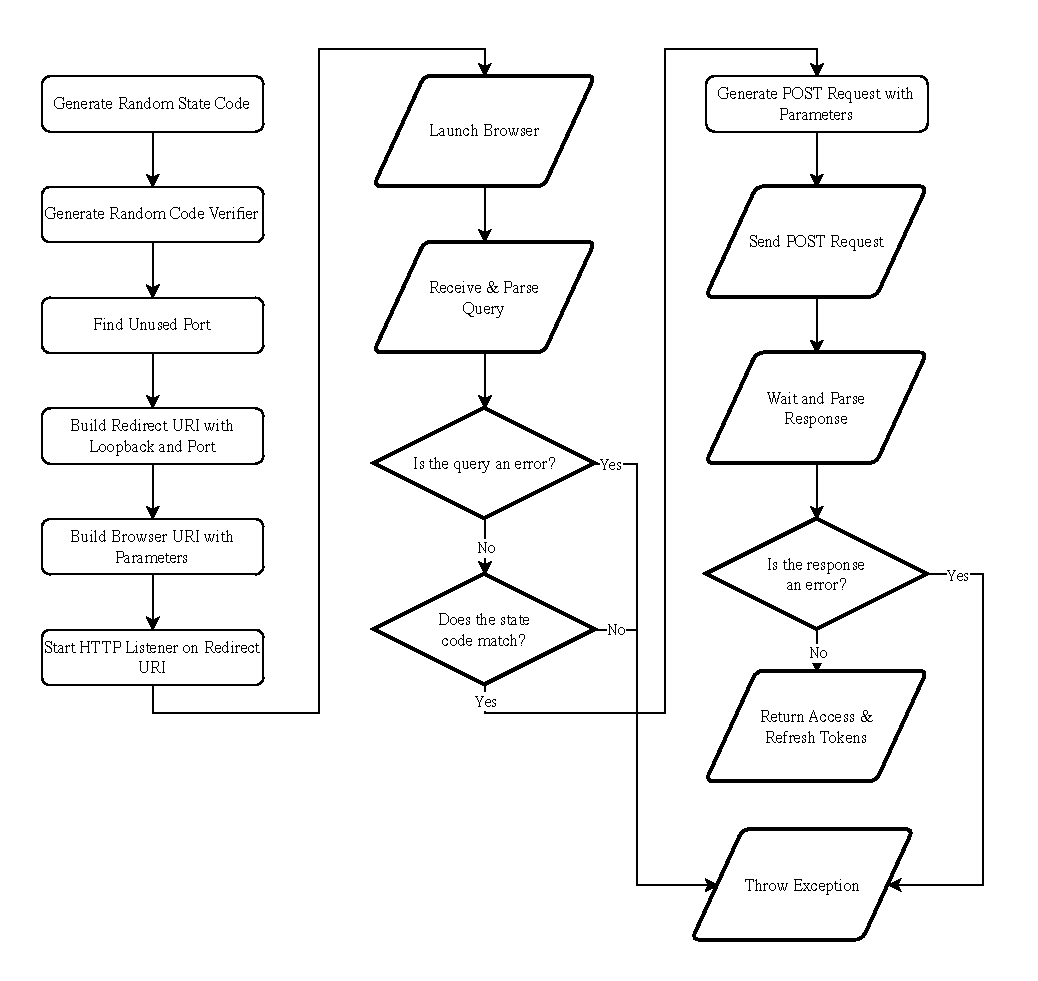
\includegraphics[width=\linewidth]{oauth-flowchart-authorisation-refresh.pdf}
    \caption{Flowchart for OAuth 2.0 Authorisation Code and New Refresh Token}
    \label{fig:oauth-flowchart-authorisation-refresh}
\end{figure}

\begin{figure}[htp]
    \centering
    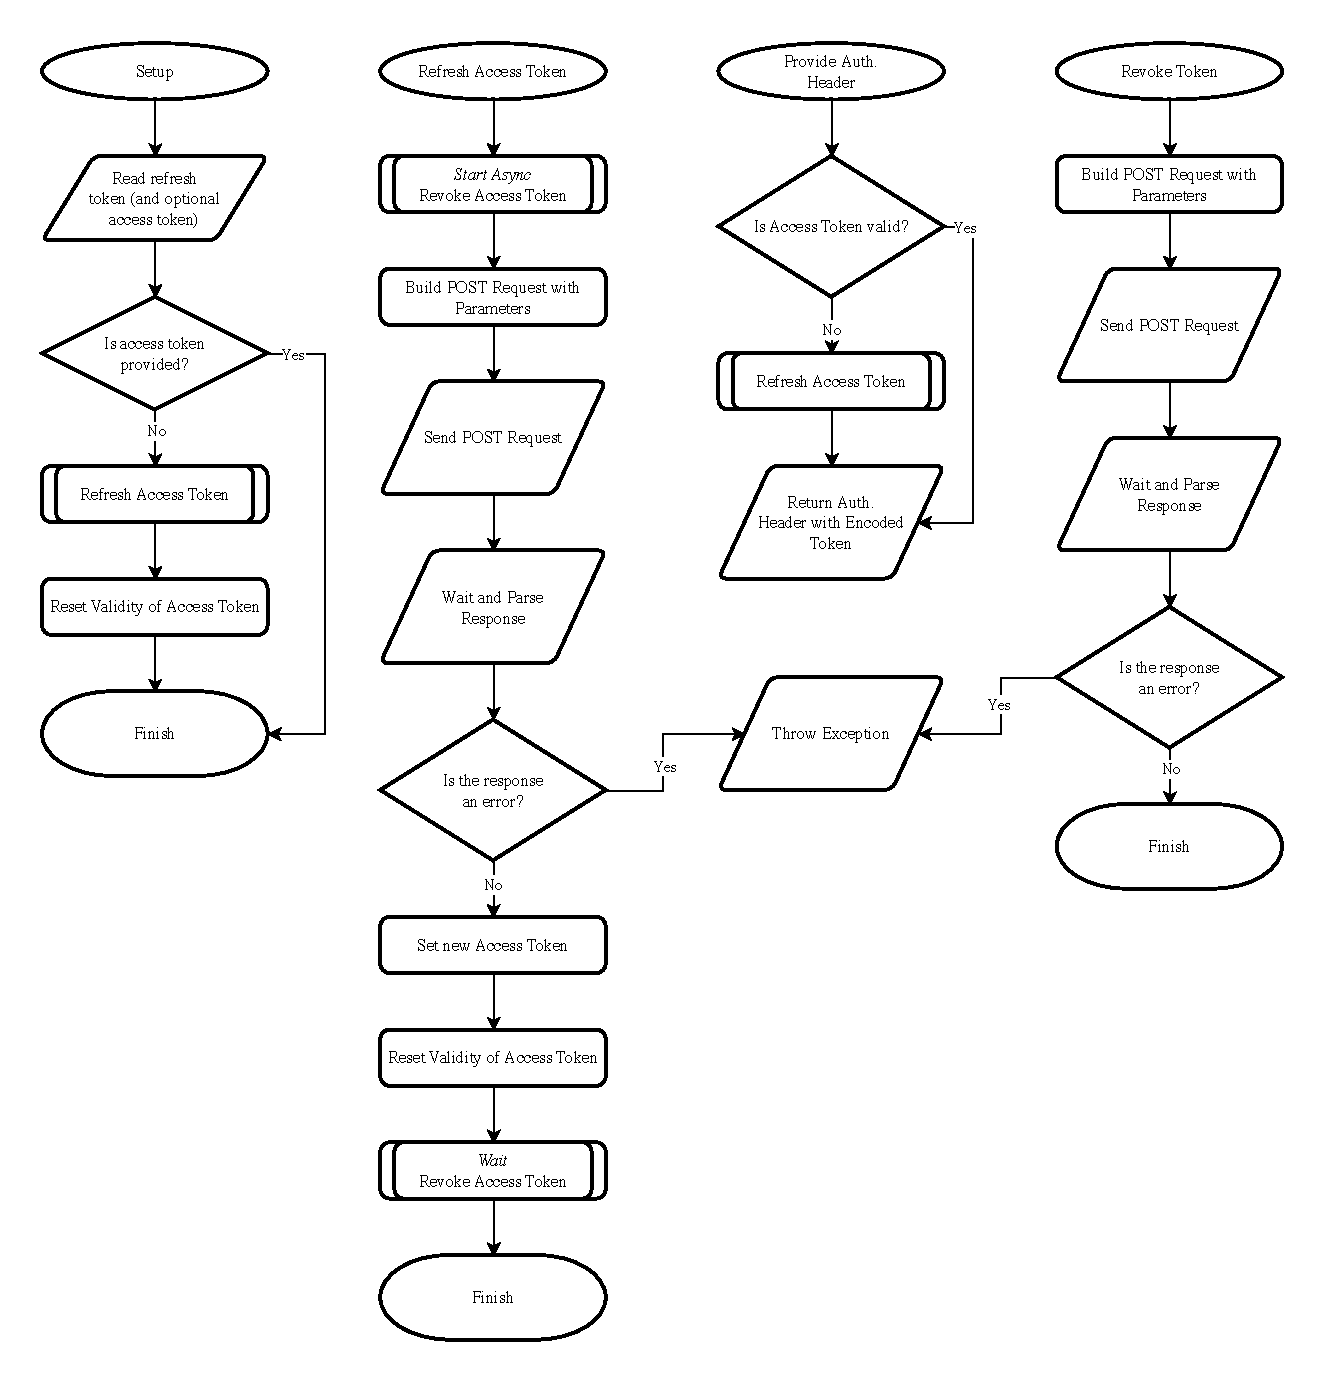
\includegraphics[width=\linewidth]{oauth-flowchart-access-check.pdf}
    \caption{Flowchart for OAuth 2.0 Acquire Access Token using Refresh Token}
    \label{fig:oauth-flowchart-access-check}
\end{figure}

Figure \ref{fig:oauth-flowchart-access-check} represents the behaviour of the OAuth2 main class for authentication, while the previous figure \ref{fig:oauth-flowchart-authorisation-refresh} represents the behaviour of the helper.

\subparagraph{Notes}

For the purposes of this NEA, we will primarily use the API Key to test the application for accessing  way of accessing DM-D.S.S. since it will be easier to code and debug, and OAuth2 will introduce quite a lot of complexity to the program. However, the program should be designed to be able to modify to OAuth2 authentication without much modification, and if time permits OAuth2 will be implemented in the application.

\subsubsection{HTTP Based API Requests}

The base URL of all requests is \url{https://api.dmdata.jp/v2/} which will be indicated as \url{base://} from now on.

Table \ref{tab:necessary-permissions} shows the necessary permissions would be necessary for the application to function. How each of them functions will be discussed below.

\begin{table}[htp]
    \centering

    \begin{tabular}{cp{0.65\linewidth}}
        Permission Code                & Permission Details                                                        \\
        \hline
        \Code{contract.list}           & Get the list of subscriptions the user has.                               \\
        \Code{gd.earthquake}           & Get list of past earthquakes.                                             \\
        \Code{parameter.earthquake}    & Get details of observation points for earthquake intensities.             \\
        \Code{socket.start}            & Start a new WebSocket connection.                                         \\
        \Code{socket.list}             & Get list of existing WebSocket connections.                               \\
        \Code{socket.close}            & Close an existing WebSocket connection.                                   \\
        % \Code{telegram.list}           & Get list of telegrams released by the JMA.                                \\
        \Code{telegram.data}           & Get specific telegram released by the JMA.                                \\
        \Code{telegram.get.earthquake} & Allows program to access telegrams on earthquake information.             \\
        \Code{eew.get.forecast}        & Allows program to access telegrams on EEW forecasts (including warnings). \\
    \end{tabular}
    \caption{Necessary access permissions for DM-D.S.S}
    \label{tab:necessary-permissions}
\end{table}

\paragraph{Standard Return Information and Errors}

There are two status that an API call could return: a successful \Code{ok} status, or an unsuccessful \Code{error} status.

Listing \ref{code:api-response-ok} shows the JSON for a successful \Code{ok} response, and Listing \ref{code:api-response-error} shows the JSON for a \Code{error} response.

\begin{listing}[htp]
    \inputminted{json}{code/ApiResponseOk.json}
    \caption{\Code{ok} status for API}
    \label{code:api-response-ok}
\end{listing}

\begin{listing}[htp]
    \inputminted{json}{code/ApiResponseError.json}
    \caption{\Code{error} status for API}
    \label{code:api-response-error}
\end{listing}

In both responses, there is an attribute \Code{responseId} which gives the unique ID for each response as a \Code{string}, and an attribute \Code{responseTime} which gives the date and time of response in \Code{ISO8601Time} format.

The \Code{status} attribute in \Code{string} indicates whether it is a successful response (in which case it will be \Code{"ok"}) and if it is an error response (in which case it will be \Code{"error"} and gives the relevant HTTP error as well). The error will be indicated in the object \Code{error} and will give the relevant message and code.

The list of standard errors together with their meanings is discussed in Table \ref{tab:standard-errors}.

\begin{table}[htp]
    \centering

    \begin{tabular}{cl}
        Error Code & Error Message                                       \\
        \hline
        \Code{400} & The query parameters are required.                  \\
        \Code{400} & The post parameters are required.                   \\
        \Code{400} & Unexpected data of search query \Code{cursorToken}. \\
        \Code{401} & Authorisation required.                             \\
        \Code{403} & Insufficient scope for ....                         \\
        \Code{403} & Requests are not allowed.                           \\
    \end{tabular}
    \caption{Standard errors for API}
    \label{tab:standard-errors}
\end{table}

The only error that might occur in the application is \Code{401} authorisation required, in the case when the OAuth 2 token expired, or the user inputted an incorrect API Key.

From here onwards, the \Code{responseId}, \Code{responseTime} and \Code{status} will be removed from the sample response by default.

\paragraph{Cursor Token}

For some API data calls, and specifically for \Code{telegram.list} that we are going to use, there is too much data to be returned in one API call. Therefore, in a response, there will be a specified attribute named \Code{nextToken} indicated with type \Code{string}, sometimes as well as \Code{nextPooloing} and \Code{nextPoolingInterval}, as shown in Listing \ref{code:cursor-token} as an example call of
\begin{center}
    \url{base://telegram?type=VXSE53}.
\end{center}

\begin{listing}[htp]
    \inputminted{json}{code/CursorToken.json}
    \caption{Cursor token sample JSON}
    \label{code:cursor-token}
\end{listing}

Specifically, the calls for \Code{socket.list} and \Code{gd.eew} will only return a \Code{nextToken} for the next call, while for \Code{telegram.list} and \Code{gd.earthquake} it will return a \Code{nextPooling} as well.

If one would like to do the next call to find the next few items of the list, the \Code{cursorToken} parameter should be specified as the same as the \Code{nextToken} or \Code{nextPooling}, with all the rest of the parameters identical to the previous request, i.e.,
\begin{center}
    \url{base://telegram?type=VXSE53&cursorToken=bmV4dCAgICAgICAgNTc0MzI}
\end{center}
if the \Code{nextToken} is used, and
\begin{center}
    \url{base://telegram?type=VXSE53&cursorToken=cG9sbGluZyAgICAgNzM0MzE}
\end{center}
if \Code{nextPooling} is used (which should be after \Code{nextPoolingInterval} in milliseconds).

The document suggested that, due to performance issues, the \Code{nextPooling} should be used wherever possible. Note that the \Code{nextToken} and \Code{nextPooling} will change for every single call of the API.

From here onwards, in the API sample results, \Code{nextToken}, \Code{nextPooling} and \Code{nextPoolingInterval} will not be included.

\paragraph{Contract API}

There is only one contract-related API, which is \Code{contract.list}. It is an HTTP GET request, on \url{base://contract} with no parameters.

It will return a list of contracts (subscriptions) of DM-D.S.S., whether or not the user has subscribed to it.

Listing \ref{code:contract-list} shows a sample return of this API call.
\begin{listing}[htp]
    \inputminted{json}{code/ContractList.json}
    \caption{Contract list sample JSON}
    \label{code:contract-list}
\end{listing}

Here, \Code{items} is the list of contracts (subscription plans), with each of its element being an object representing a plan. For each of them, there are the properties:
\begin{itemize}
    \item \Code{id} (nullable) which stands for the subscription ID (could be \Code{null} if the user is not subscribed);
    \item \Code{planId} which stands for the subscription plan ID, which is unique for each plan;
    \item \Code{planName} which stands for the name of the subscription plan;
    \item \Code{classifications} which stands for the classification code of the subscription plan;
    \item \Code{price.day} and \Code{price.month} which stands for the price of the plan per day/per month;
    \item \Code{start} (nullable) which stands for the start of the subscription;
    \item \Code{isValid} which is a \Code{boolean} to represent whether the plan is valid; and
    \item \Code{connectionCounts} which stands for the number of extra WebSocket connections this subscription plan provides.
\end{itemize}

Note that how \Code{id} and \Code{start} can be \Code{null} since it lists all the subscriptions, whether or not the user has been subscribed to it.

This API will be used to calculate the number of WebSocket connections, to display empty WebSocket slots in the listing WebSocket functionality.

\paragraph{WebSocket APIs}

There are three WebSocket-Related APIs, specifically, \Code{socket.start}, to start a socket, \Code{socket.list} to list all sockets, and \Code{socket.close}, to close a socket. They are all called on \url{base://socket}.

\subparagraph{Socket Start}

\Code{socket.start} is a POST method which has a request body in JSON, as shown in Listing \ref{code:socket-start-post}.

\begin{listing}[htp]
    \inputminted{json}{code/SocketStartPost.json}
    \caption{Socket start sample request JSON}
    \label{code:socket-start-post}
\end{listing}

The attributes are:
\begin{itemize}
    \item \Code{classifications}, which is a list of classifications of the subscription plans (which include all the types below);
    \item \Code{types} (optional), which is a list of telegram wished to be transmitted through the WebSocket;
    \item \Code{test} (optional, default to \Code{"no"}), which indicates whether test telegrams should be received (\Code{"including"}) or not (\Code{"no"});
    \item \Code{appName} (optional), which is the name of the application to be recorded with the WebSocket; and
    \item \Code{formatMode} (optional, default to \Code{"raw"}), which is either \Code{"json"} or \Code{"raw"} depending on the desired return type.
\end{itemize}

The detailed classifications and types will be discussed in the next section on WebSocket connections. When the \Code{types} is excluded, the WebSocket will return all the telegrams included in the classification.

It will have a response as in Listing \ref{code:socket-start}.

\begin{listing}[htp]
    \inputminted{json}{code/SocketStart.json}
    \caption{Socket start sample response JSON}
    \label{code:socket-start}
\end{listing}

Some attributes are exactly the same as the JSON sent has header, \Code{classifications}, \Code{types} (nullable), \Code{test} and \Code{appName}. The additional attributes are:
\begin{itemize}
    \item \Code{ticket}, which is a code in \Code{string} for the connection. This is also included in the \Code{websocket} object.
    \item \Code{websocket}, which is the object containing details for the connections. Its attribute \Code{id} is unique for each connection and \Code{url} is the WebSocket (\Code{wss://}) URL to use to connect to. \Code{protocal} being a constant array containing \Code{"dmdata.v2"} indicating that this is the 2nd version of the protocol. \Code{expiration} is in seconds the time the connection will expire if no transmission handshakes are made (see below), and is always \Code{300} as constant.
    \item \Code{formats}, which is a list of formats used to encode the data transmitted in the WebSocket. This is a constant list including \Code{"xml"}, \Code{"a/n"} and \Code{"binary"} if \Code{formatMode} is set to \Code{"raw"}, and a list with only \Code{"json"} if set to \Code{"json"} in the request JSON.
\end{itemize}

Apart from the standard errors, it will also output errors shown in Table \ref{tab:socket-start-err}

\begin{table}[htp]
    \centering

    \begin{tabular}{cl}
        Error Code & Error Message                                                       \\
        \hline
        \Code{400} & The body of the request is not JSON.                                \\
        \Code{400} & At least one element of \Code{classifications} is required.         \\
        \Code{400} & The \Code{types} is not a string or has more than 30 elements.      \\
        \Code{400} & The \Code{appName} is up to 24 bytes.                               \\
        \Code{400} & You have entered a string that is not defined in \Code{formatMode}. \\
        \Code{402} & No contract.                                                        \\
        \Code{409} & The maximum number of simultaneous connections is exceeded.         \\
    \end{tabular}
    \caption{Errors for \Code{socket.start}}
    \label{tab:socket-start-err}
\end{table}

The only error that should occur in the application is the final one, where the maximum number of simultaneous connections is exceeded. To allow the user to deal with this situation, a disconnect button for each connection in the current WebSocket list is provided.

\subparagraph{Socket Close}

\Code{socket.close} is a DELETE method, which specifies the ID of the WebSocket port to be closed in the URL parameter \Code{:id}, e.g., \url{base://socket/30}. If the result is successful, the request will not return anything. If the status is error, it will return a standard error (detailed above), or a \Code{404} error, which indicates that the specified WebSocket \Code{id} is not found.

There is a chance of a \Code{404} error for WebSocket ID not found, if the list has not been refreshed, and the user attempts to disconnect to the WebSocket which was already disconnected. Due to this, the refresh WebSocket list button is provided should such error occur.

\subparagraph{Socket List}

\Code{socket.list} is a GET method which supports \Code{cursorToken} (optional) as discussed above. There are other parameters in the query:
\begin{itemize}
    \item \Code{id} (optional), which stands for the ID of the WebSocket connection that details is wished to be retrieved;
    \item \Code{status} (optional), a \Code{string} indicating the status of the WebSocket, including \Code{open} which stands for operating live, \Code{waiting} which means idle, and \Code{closed} standing for closed connections;
    \item \Code{limit} (optional, default 20), of type \Code{integer} with a maximum of 100, indicating the number of WebSockets listed in a single response.
\end{itemize}

Listing \ref{code:socket-list} shows a response from the call. The \Code{items} is a list of objects, each representing a WebSocket, with the following properties:
\begin{itemize}
    \item \Code{id}, \Code{ticket}, \Code{classifications}, \Code{test}, \Code{types}, \Code{formats}, \Code{appName}, identical to described above;
    \item \Code{start}, a \Code{ISO0601Time} representing the time of the start of the connection;
    \item \Code{end}, a nullable \Code{ISO0601Time} representing the time of the end of the connection;
    \item \Code{ping}, a nullable \Code{ISO0601Time} representing the previous time of ping-pong;
    \item \Code{ipAddress}, a nullable \Code{string} representing the IP address of the source of connection;
    \item \Code{server}, a nullable \Code{string} representing the connected WebSocket server; and
    \item \Code{status}, a \Code{string} representing the connection status.
\end{itemize}

\begin{listing}[htp]
    \inputminted{json}{code/SocketList.json}
    \caption{Socket list sample response JSON}
    \label{code:socket-list}
\end{listing}

However, it is worth noting that even though the document claims that \Code{ticket} is not \Code{null}, it will only be not null when the WebSocket is waiting connection, and null otherwise. Furthermore, \Code{formats} never appears in the result, even though the document claims that it should always appear.

These API calls will be used to manage (open new, list existing and close) WebSockets in the application.

\paragraph{Parameter API}

The program would need to have a list of observation points of earthquakes to plot on the map the observed stations' intensity on the past-page map. Therefore, we would need to call \Code{parameter.earthquake}, which is available at \url{base://parameter/earthquake/station}.

This is a GET request with no parameters to specify, and will return all stations in one go (which is time-costly). Listing \ref{code:parameter-earthquake} shows a sample response.

\begin{listing}[htp]
    \inputminted{json}{code/ParameterEarthquake.json}
    \caption{Earthquake parameter sample response JSON}
    \label{code:parameter-earthquake}
\end{listing}

The \Code{changeTime} and \Code{version} of this list of parameters is often the same for calls since the list is rarely updated, and they give the version of the list and the last time of the update.

For each object in \Code{items}, they represent an earthquake observation point. The attributes are:
\begin{itemize}
    \item \Code{region} and \Code{city}, both containing \Code{code}, \Code{name} and \Code{kana} (Kana (カナ, 仮名) represents the pronunciation), which is unique for each region and city;
    \item \Code{noCode}, the unique code, and \Code{code}, the code used in XML (WebSocket data feeds);
    \item the \Code{name} and \Code{kana}, which are not necessarily unique for each observation point;
    \item \Code{status} standing for whether the station is in use. \Code{"現"} (now) means the data hasn't changed in the update, \Code{"変更"} (change) means the data has been altered, \Code{"新規"} (new) stands for a new observation point, and \Code{"廃止"} (abolished) means the observation point has been discontinued;
    \item the \Code{owner}, representing the owner of the observation point; and
    \item the \Code{latitude} and \Code{longitude}, which as the name suggests, represent the position of the observation point.
\end{itemize}

Due to the nature of JSON being very long and barely updated (an email will be sent to users of DM-D.S.S. every time its updated in fact), it will be obtained upon application launch/authentication by the user, and stored in the main memory for the lifetime of the application, rather than obtaining such every time when necessary.

% \paragraph{Telegram API}

% JMA release telegrams (mostly in XML format) through DM-D.S.S., and to achieve them, we can use the \Code{telegram.list} GET request, which is available at \url{base://telegram}. It supports \Code{cursorToken} with pooling.

% Furthermore, the following query parameters are available:
% \begin{itemize}
%     \item \Code{type} (optional), which indicates the type of telegram wishing to retrieve. Note that there can be a maximum of 5 types of telegrams specified due to the need for a perfect match;
%     \item \Code{xmlReport} (optional, default \Code{false}), which specifies whether some details of the XML report should be included in the JSON;
%     \item \Code{test} (optional, default \Code{no}), which specifies whether test telegrams should be included. Options are \Code{no}, \Code{including} and \Code{only};
%     \item \Code{formatMode} (optional, default \Code{raw}) indicates whether the XML reports should be converted to JSON;
%     \item \Code{limit} (optional, default 20) indicates the number of telegrams returned in one response.
% \end{itemize}

% Listing \ref{code:telegram-list} gives a sample response of this API call.

% \begin{listing}[htp]
%     \inputminted{json}{code/TelegramList.json}
%     \caption{Telegram list sample response JSON}
%     \label{code:telegram-list}
% \end{listing}

% In the \Code{items} list, each object represents a telegram, with certain properties:
% \begin{itemize}
%     \item \Code{serial} stands for the serial ID of this transmission, while \Code{id} is a unique ID for the telegram (non-serial);
%     \item \Code{classification} gives the classification of this telegram. For the purpose of this application, all classification will be of type \Code{telegram.earthquake};
%     \item \Code{head} gives the head of this telegram, including the \Code{type}, the \Code{author}, the \Code{time}, and whether it is \Code{test};
%     \item \Code{receivedTime} gives the time of this telegram being released,
%     \item \Code{xmlReport} details parts of information encoded in the XML, if the \Code{xmlReport} option in the query is set to true;
%     \item \Code{url} gives the URL for the detailed information of this telegram (that can be retrieved using another GET request), and \Code{format} gives its format.
% \end{itemize}

% Apart from standard errors, it might also return a \Code{400} error with message 'You have entered a string that is not defined in \Code{formatMode}.'

\paragraph{Past Earthquake API}

The API \Code{gd.earthquake} allows us to use a GET request to obtain a series of earthquake on \url{base://gd/earthquake}, with the option to obtain a list, or to obtain only a certain event.

\subparagraph{Past Earthquake List} The API call \Code{gd.earthquake.list}, which supports \Code{cursorToken} and \Code{poolingToken} allows us to obtain a list of past earthquakes, with the ability to specify the following parameters:
\begin{itemize}
    \item \Code{hypocenter}, the 3-digit code to filer the hypocentre position;
    \item \Code{maxInt}, the lower bound of the filter for the maximum measured intensity of the earthquake;
    \item \Code{date}, the date when the earthquake is observed;
    \item \Code{limit}, the number of earthquakes returned in one go, with a maximum of 100.
\end{itemize}

A sample response is shown in Listing \ref{code:earthquake-list}.

\begin{listing}[htp]
    \inputminted{json}{code/GdEarthquakeList.json}
    \caption{Past earthquake list sample response JSON}
    \label{code:earthquake-list}
\end{listing}

These APIs will be used to display a list of past earthquakes. For each object representing an earthquake, this includes:
\begin{itemize}
    \item Its unique \Code{id}, \Code{eventId}, \Code{originTime} (if it is not a report on the intensity), and \Code{arrivalTime};
    \item its \Code{type} (which is \Code{normal} for earthquakes in Japan, and \Code{distant} for earthquake reported by other countries);
    \item its \Code{hypocenter}, including the \Code{code}, \Code{name}, the \Code{coordinate} and the \Code{depth};
    \item its \Code{magnitude} (an object representing units and values); and
    \item its \Code{maxInt}, the maximum intensity observed.
\end{itemize}

It might also include LPGM information, in \Code{maxLgint} and \Code{lgCategory}, if such information is released, usually only for huge earthquakes.

The data used will be used to create the sidebar (list of past earthquakes) of the past page in the application, and will be called upon the click of refresh button/load more button.

\subparagraph{Past Earthquake Event} If the call \url{base://gd/earthquake/:eventId} is used, it will return the object representing the earthquake in the \Code{event} attribute (most attributes removed since identical to Listing \ref{code:earthquake-list}), as well as a list of telegrams in the \Code{telegrams} attribute, which was detailed above in the \Code{telegram.list} section, as shown in Listing \ref{code:earthquake-event}.

\begin{listing}[htp]
    \inputminted{json}{code/GdEarthquakeEvent.json}
    \caption{Past earthquake event sample response JSON}
    \label{code:earthquake-event}
\end{listing}

In the \Code{telegrams} list, each object represents a telegram, with certain properties:
\begin{itemize}
    \item \Code{serial} stands for the serial ID of this transmission, while \Code{id} is a unique ID for the JSON telegram (non-serial);
    \item \Code{originalId} gives the original ID of the telegram in XML format;
    \item \Code{classification} gives the classification of this telegram. For the purpose of this application, all classification will be of type \Code{telegram.earthquake};
    \item \Code{head} gives the head information of this telegram, including the \Code{type}, the \Code{author}, the \Code{time}, and whether it is \Code{test};
    \item \Code{receivedTime} gives the time of this telegram being released,
    \item \Code{xmlReport} details parts of information encoded in the XML;
    \item \Code{schema} details the JSON schema used for the telegram, including the \Code{type} and \Code{version} of the schema used;
    \item \Code{url} gives the URL for the detailed information of this telegram (that can be retrieved using another GET request), and \Code{format} gives its format.
\end{itemize}

All telegrams provided in this list are in JSON format.

This API will be used to load the details for a certain earthquake to display on the sidebar panel.

\subsubsection{WebSocket Connections}

WebSocket connections are essential to real-time applications, since it provides a real-time feed from the server to the client on latest data, without the need of the client to query (which consumes a lot of resources). DM-D.S.S. provides WebSockets to initiate real-time connection to the server to achieve the latest telegrams and earthquake warnings.

The URL of the WebSocket will be \url{wss://{#1}.api.dmdata.jp/v2/websocket}, where the \Code{#1} part could be \Code{ws001} to \Code{ws004}, but it is optional. If not included, the server will simply distribute the load.

\paragraph{WebSocket Responses}

There are four types of responses that a WebSocket could return, indicated in the \Code{type} attribute:
\begin{itemize}
    \item a \Code{start}. This only happens when the WebSocket is started, and this includes the exact same information in the \Code{socket.start} call in Listing \ref{code:socket-start}, with an additional \Code{time} to indicate the time of the response;
    \item a (server-side initiated) \Code{ping}. This will happen regularly, and the server will send a JSON in the format in Listing \ref{code:server-ping}.
          \begin{listing}[htp]
              \inputminted{json}{code/ServerPing.json}
              \caption{WebSocket Ping JSON}
              \label{code:server-ping}
          \end{listing}

          Upon receiving, the client should return a \Code{pong} JSON in the same format, with the same \Code{pingId}, as in Listing \ref{code:server-pong}.

          \begin{listing}[htp]
              \inputminted{json}{code/ServerPong.json}
              \caption{WebSocket Pong JSON}
              \label{code:server-pong}
          \end{listing}

          This is in place to ensure that there are no 'dead' WebSocket connections, and the server will close the WebSocket connection after 120s of no response in such ping-pong calls, to not take up the limited number of WebSocket connection slots;
    \item a client-side initiated \Code{ping} as in Listing \ref{code:server-ping}, which the server will return a \Code{pong} as in Listing \ref{code:server-pong}. This works almost identically as before, apart from that such \Code{pingId} is optional. This is in place to ensure that the application would be able to know if the connection is broken, for example due to unstable internet connections, and would be able to restart another WebSocket connection;
    \item a \Code{error}, which will be the format in Listing \ref{code:socket-error}. There will also be a boolean, \Code{close}, to indicate whether the WebSocket connection is closed or not.

          \begin{listing}[htp]
              \inputminted{json}{code/SocketError.json}
              \caption{WebSocket Error JSON}
              \label{code:socket-error}
          \end{listing}

          A table of possible WebSocket errors is included in \ref{tab:socket-error}, with the relevant WebSocket error codes.

          \begin{table}[htp]
              \centering

              \begin{tabular}{cl}
                  Error Code  & Error Details                                                    \\
                  \hline
                  \Code{4400} & Compulsory parameters are not specified when starting WebSocket. \\
                  \Code{4404} & Ticket is not specified when starting WebSocket.                 \\
                  \Code{4409} & Number of connection limit is reached.                           \\
                  \Code{4503} & Internal server error.                                           \\
                  \Code{4640} & \Code{pingId} does not match for a server-initiated \Code{ping}. \\
                  \Code{4641} & Incorrect data (non-JSON) received from client.                  \\
                  \Code{4808} & Client requested closure of WebSocket.                           \\
                  \Code{4807} & Contracts are discontinued in connection.                        \\
              \end{tabular}
              \caption{Errors for WebSocket connection}
              \label{tab:socket-error}
          \end{table}

          In the application, only \Code{4409} (when the connection number exceeded the maximum), \Code{4503} (when the server has an internal error), \Code{4808} (when the client requested closure of WebSocket), and \Code{4807} (contract discontinued) should occur in the application.

          The program should be designed to be able to handle these errors, and to close the connection if necessary;
    \item a \Code{data}, an example shown in Listing \ref{code:socket-data}.
          \begin{listing}[htp]
              \inputminted{json}{code/SocketData.json}
              \caption{WebSocket Data JSON}
              \label{code:socket-data}
          \end{listing}

          This will include a \Code{classification}, a version \Code{version}, and a unique \Code{id}. A list named \Code{passing} gives the \Code{name} and \Code{time} of each passing location of this data piece inside the server.

          Furthermore, the \Code{head} and \Code{xmlReport} gives details of the telegram received, similar to in Listing \ref{code:earthquake-event}.

          The \Code{format}, \Code{compression} (\Code{gzip}, \Code{zip} or \Code{null}) and \Code{encoding} (\Code{base64} or \Code{utf-8}) gives information on how the \Code{body} should be processed and interpreted.

          Note that the body should always be dealt with in the following sequence: decode; decompress; and deserialise.

          This gives the key piece of information that will be passed between the data component of the software and the UI component of the software.
\end{itemize}

\paragraph{JSON v.s. XML}

Most data nowadays on the internet are serialised in JSON, but the JMA provides its data in XML format. DM-D.S.S. does also provide JSON formatted schemas for most of the XML data files which are also processed real time. Even though there is a high chance of delay (up to 1 second) if the JSON format is used, not to say the potential of an error in processing which lead to undefined behaviour in the JSON format, the JSON format is much easier to parse and deserialise into C\# DTO objects, and the schemas are very well-defined on the DM-D.S.S. references \autocite{dmdata-references-json}, in contrast to the JMA documentation \autocite{jma-xml-format} which is in Japanese (which the author is not an expert in). Therefore, JSON format telegrams and data will be used in the application.

\paragraph{Design of WebSocket Wrapper}

.NET has a built-in sealed \Code{ClientWebSocket} class, and therefore to use it, we would have to wrap a class around it (i.e. a class that composites \Code{ClientWebSocket} class), since it is responsible for the life-cycle of the WebSocket as well. The wrapper is re-used over multiple connections, while the backing \Code{ClientWebSocket} class is disposed per-use.

Events are used here (Data Received and Status Changed) to use callbacks to send back the data to the necessary component, such as the View Model for the GUI (introduced later). Furthermore, the FIFO data structure queue is used to store pings sent by the client, since a later ping received would indicate that the connection is still alive, and the ping, together with all pings before that ping (and including that ping itself), could be removed from the queue.

The overall flow structure is shown in Figure \ref{fig:websocket-flowchart} for the overall functionality of the WebSocket flowchart, and in Figure \ref{fig:websocket-response} for dealing with the received response.

\begin{figure}
    \centering
    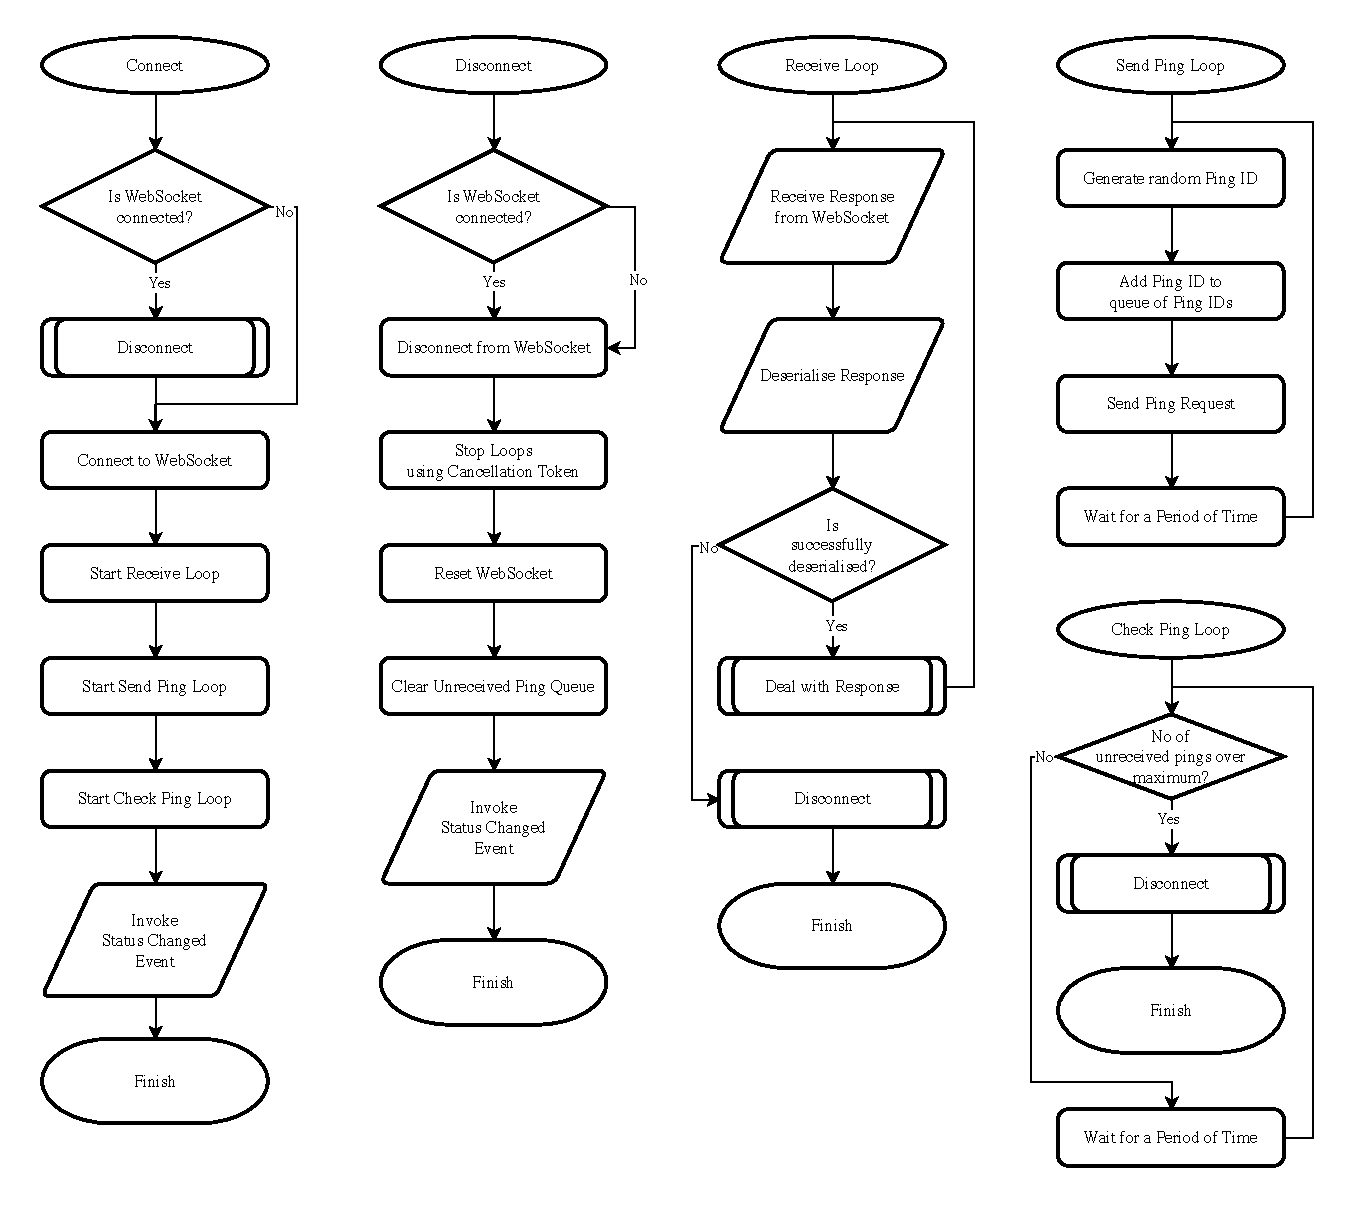
\includegraphics[width=\linewidth]{websocket-flowchart.pdf}
    \caption{Flowchart of WebSocket Wrapper}
    \label{fig:websocket-flowchart}
\end{figure}

\begin{figure}
    \centering
    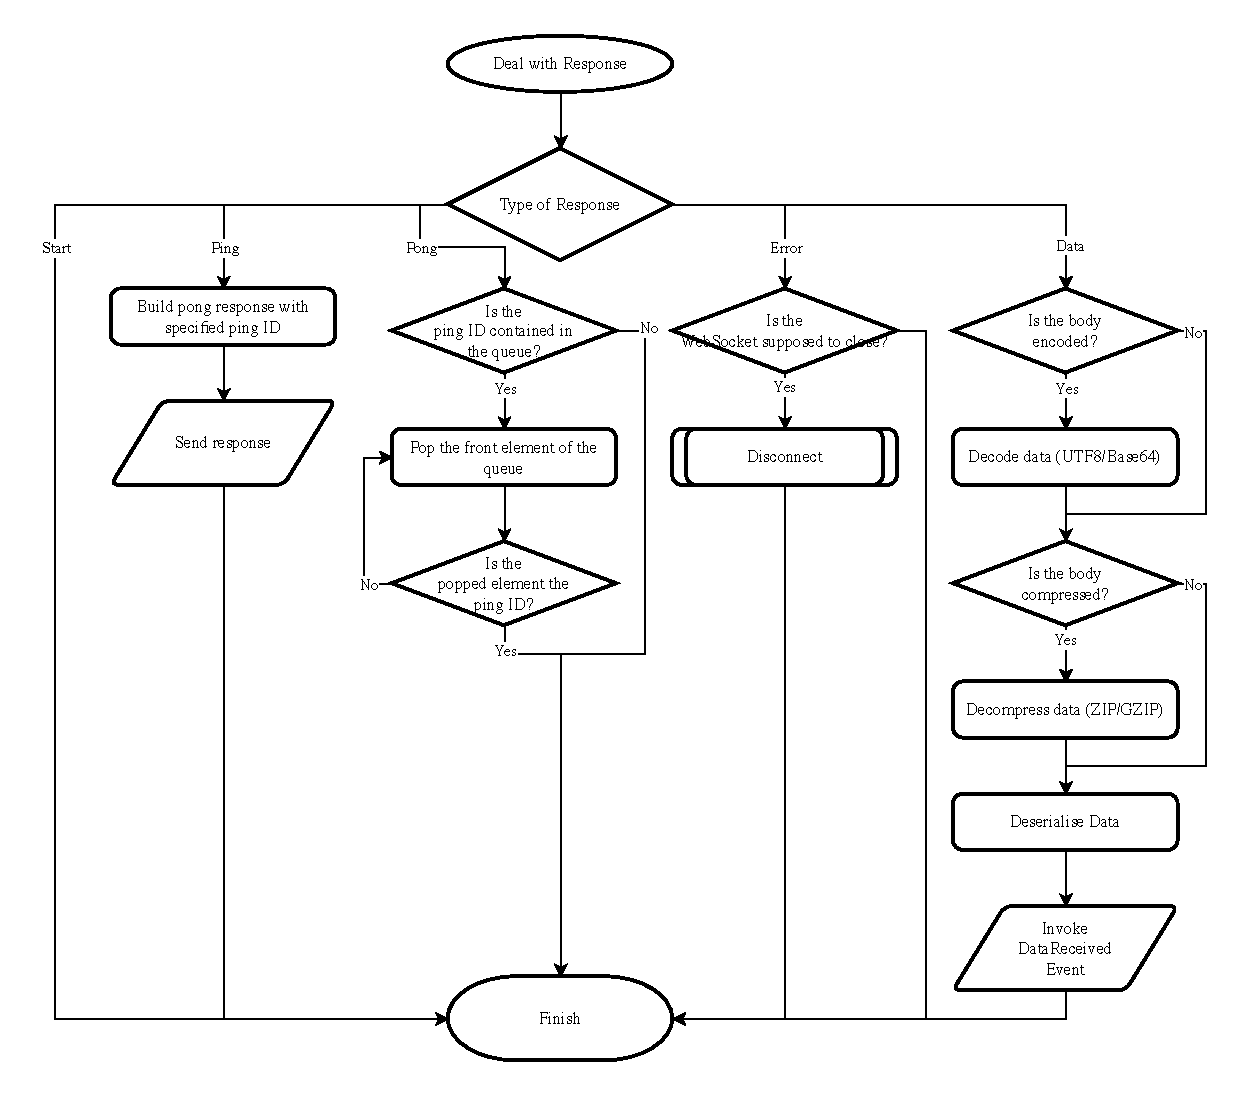
\includegraphics[width=\linewidth]{websocket-response.pdf}
    \caption{Flowchart of dealing with WebSocket Response}
    \label{fig:websocket-response}
\end{figure}

\subsubsection{Telegrams}

As discussed in the previous section, JSON telegrams is going to be used in the application, and there is no particular reason why telegrams in general (i.e. for the earthquake telegrams in \Code{gd.earthquake.event} for the past-page) should be retrieved in XML format compared to JSON format. In this section we will discuss the telegrams used, and the structure of a telegram in DM-D.S.S.

\paragraph{Telegrams Used}

Considering the uses of the application, Table \ref{tab:telegrams-used} gives an overview of the telegrams used in the application.

\begin{table}[htp]
    \centering
    \begin{tabular}{cccp{15em}}
        Code   & Telegram Classification    & JSON Schema                   & Description                                                 \\
        \hline
        VXSE45 & \Code{eew.forecast}        & \Code{eew-information}        & All EEW telegrams including forecasts and warnings.         \\
        VXSE51 & \Code{telegram.earthquake} & \Code{earthquake-information} & Preliminary report on the measured intensity of earthquake. \\
        VXSE52 & \Code{telegram.earthquake} & \Code{earthquake-information} & Preliminary report on the hypocentre of earthquake.         \\
        VXSE53 & \Code{telegram.earthquake} & \Code{earthquake-information} & Full report on intensity and hypocentre of earthquake.      \\
        VTSE41 & \Code{telegram.earthquake} & \Code{tsunami-information}    & Tsunami warnings of all types.
    \end{tabular}
    \caption{Telegrams used in the application}
    \label{tab:telegrams-used}
\end{table}

In the real-time page, VXSE45 and VTSE41 telegrams are fed via the WebSocket connection detailed above to be displayed. On the past page, VXSE51~53 telegrams are used to display the past earthquake information. In specific, the following logic will be used to determine which telegram to use: (in the following, \(x = 1, 2, 3\))
\begin{itemize}
    \item Filter the telegram to only include VXSE5\(x\);
    \item Group telegrams by the telegram code;
    \item Find the latest telegram (by serial number) in each of the category;
    \item Use the telegram with the biggest \(x\) (i.e. VXSE53 > VXSE52 > VXSE51).
\end{itemize}

The particular choice for the final one is due to the fact that VXSE53 usually contains the most information, while VXSE51 and VXSE52 usually contains less information than VXSE53. (They are usually released earlier than VXSE53 though).

\paragraph{JSON Schemas}

All JSON Schemas include a part called the \textbf{schema head}, and a sample is shown in Listing \ref{code:telegram-head}.

\begin{listing}[htp]
    \inputminted{json}{code/TelegramHead.json}
    \caption{Head of JSON Schema}
    \label{code:telegram-head}
\end{listing}

There are the following properties:
\begin{itemize}
    \item \Code{_originalId}, the original ID of the telegram;
    \item \Code{_schema}, the DM-D.S.S. JSON Schema used for this telegram, including the type and the version;
    \item \Code{type}, the name of the telegram, and \Code{title}, the title of the telegram;
    \item \Code{status}, the status of the telegram, whether it is normal (\Code{通常}), a training telegram (\Code{訓練}), or a test telegram (\Code{試験}). Note that telegrams should be filtered in the application to only display normal telegrams to the user;
    \item \Code{infoType}, the type of information, whether it is a release (\Code{発表}), a correction (\Code{訂正}), a delay (\Code{遅延}), or a cancellation (\Code{取消}). Note that in EEW telegrams, there is also an indication in the \Code{body} part whether it is a cancellation;
    \item \Code{editorialOffice}, and a list of \Code{publishingOffice};
    \item \Code{pressDateTime} when the telegram is made, \Code{reportDateTime} when the telegram is released;
    \item \Code{targetDateTime} which is nullable, describes the base time of the report, and \Code{targetDatetimeDubious} giving the error;
    \item \Code{validDateTime} for which the report is valid until (e.g. for tsunami information, there will not be cancellation reports, only a date time the information is valid until);
    \item \Code{eventId}, the unique ID for the event that this describes. This should be used to identify earthquakes in the EEW;
    \item \Code{serialNo}, the number that is released for the specific event. In EEW, if a telegram with lower serial is received after a telegram with a higher serial (e.g. due to delay reasons), then the telegram should not be used and should be disposed of;
    \item \Code{infoKind} and \Code{infoKindVersion}, the schema used in the XML report;
    \item \Code{headline}, which includes the summary headline of the information;
    \item \Code{body}, the body of all the information.
\end{itemize}

In particular, the information of \Code{_schema}, \Code{status}, \Code{pressDateTime} (for displaying the last updated time of the information), \Code{eventId}, \Code{serialNo} and the \Code{body} will be useful for the application.

The \Code{body} part of the telegram will be omitted for brevity, since they are mostly just convoluted JSON objects. Anything interesting in particular will be mentioned later in the design for the DTOs.

\subparagraph{Text and Comments component of the body} For all schemas used in the application, in the \Code{body} component, there will be properties \Code{text} (of type string) and \Code{comments} which includes text and comments on the telegram.

In the \Code{comments} property, there could always be a \Code{free} property where any string could be recorded, and some other properties (whose names may vary: \Code{warning} for \Code{tsunami-information} and \Code{eew-information}, and \Code{forecast} and \Code{var} for \Code{earthquake-information}), each containing a list of strings and codes which are paired, where the code is a 3-digit code representing the code of the comment.

An example of this is shown in Listing

\begin{listing}[htp]
    \inputminted{json}{code/TelegramComments.json}
    \caption{Comments in JSON Schema}
    \label{code:telegram-comments}
\end{listing}

These should be used, together with the headline property, to create the informational text to display with a telegram.

\subsubsection{Sidenotes}

It is worth noting that an existing NuGet Library, \GitHubHref{ingen084}{DmdataSharp} supports dealing with the DM-D.S.S. data flow and converting them to C\# objects (and exceptions). However, for the purposes of this NEA, we will implement our own way to interact with the APIs and the correlated C\# DTOs. The developer of this library did also mention that it is quite purpose-built so might not be suitable for general use.

This section referred to \autocite{dmdata-references-api, dmdata-references-json, dmdata-references-oauth, dmdata-references-telegram}.

\section{Algorithms}

There are two key 'algorithms' that was designed for this application (in addition to the inverse-cubic for converting colours as described previously): the first one used to calculate the position of the P/S wavefronts, and the other one used to detect shake on the real-time monitoring screen.

\subsection{Wavefront Calculation}

Earthquake waves do not travel at uniform rate as they spread out due to the decrease in energy, and so there is no uniform velocity that the seismic waves travel in. We cannot do a simple equation like \(s = vt\) to calculate the distance of the wavefront of a seismic wave from the epicentre.

However, JMA provides tables for the time that seismic waves take to travel a certain distance in \autocite{jma-timetable-2001}, together with \autocite{jma-timetable-format}. It will be possible for us to look up the table and plot the seismic waves at correct distance at a certain time.

Comparing the different wave travel tables that JMA provides, the most suitable one for this application will be the \textbf{JMA 2001}, since it is designed for general purpose uses for both land-based and ocean-based earthquakes, and does not take into account the effect of the altitude of the observation points. Listing \ref{code:jma-2001} provides a preview of the first 10 lines of this file.

\begin{listing}[htp]
    \inputminted[lastline=10,showspaces]{text}{code/tjma2001.txt}
    \caption{JMA 2001 Wave Travel Tables}
    \label{code:jma-2001}
\end{listing}

The table is a lookup table from horizontal distance to time in terms of the depth of the epicentre and the type of wave (P or S) to the time needed to travel such distance. Each row represents the P-Wave, time taken for the P-wave to travel (in seconds), S-wave, time taken for the S-wave to travel (in seconds), depth of epicentre (in kilometres), distance from epicentres (in kilometres).

This file will be read by the program upon launch every time and stored in the active memory when the program is running.

\subsubsection{Format of Rows}

The format of the table is as follows:
\begin{itemize}
    \item \textbf{Column 1.} The wave (P);
    \item \textbf{Column 2.} Whitespace;
    \item \textbf{Column 3-10.} The time in seconds, with exactly 4 characters (whitespace padding to the left) before the decimal point, and 3 after;
    \item \textbf{Column 11.} Whitespace;
    \item \textbf{Column 12.} The wave (S);
    \item \textbf{Column 13.} Whitespace;
    \item \textbf{Column 14-21.} The time in seconds, with exactly 4 characters (whitespace padding to the left) before the decimal point, and 3 after;
    \item \textbf{Column 22.} Whitespace;
    \item \textbf{Column 23-25.} The depth of the epicentre in kilometres, with spaces padding to the left;
    \item \textbf{Column 26-27.} Whitespace;
    \item \textbf{Column 28-32.} The distance from the epicentre in kilometres, with spaces padding to the left.
\end{itemize}

Therefore, the following regular expression is designed to match each row (with the \^ anchor at the start, and \$ anchor at the end):
\begin{center}
    \Code{P ((?=.{4}) *\d+)\.\d{3} S ((?=.{4}) *\d+)\.\d{3} ((?=.{3}) *\d+)  ((?=.{5}) *\d+)}
\end{center}

Most part of this is quite straightforward, but it is worth explaining what \Code{((?=.{x}) *\d+)} means here. The \Code{(?=.{x})} is a positive lookahead looking \(x\) digits afterwards, but it is not really part of the match. The pattern \Code{ *\d+} is the pattern that this lookahead should match to. Therefore, \Code{((?=.{x}) *\d+)} matches to a number that has left padding to reach exactly \(x\) digits, which is exactly what is required for the numbers in the time, depth and distance column, providing the matching for the padding.

\subsubsection{Format of Table}

The depth and the distance from epicentre is provided in the intervals specified in \ref{tab:dist-jma-2001}. They are provided for distances up to 2000 kilometres and depths up to 700 kilometres.

\begin{table}[htp]
    \centering

    \begin{tabular}{ccc}
        Distance                  & Interval for Depth & Interval for distance \\
        \hline
        0 \textasciitilde\ 50     & 2                  & 2                     \\
        50 \textasciitilde\ 200   & 5                  & 5                     \\
        200 \textasciitilde\ 700  & 10                 & 10                    \\
        700 \textasciitilde\ 2000 & --                 & 10
    \end{tabular}
    \caption{Distance intervals in JMA 2001}
    \label{tab:dist-jma-2001}
\end{table}

The table is ordered in increasing order of depth, then by distance. This means that there are
\[
    \frac{50}{2} + \frac{200 - 50}{5} + \frac{700 - 200}{10} + \frac{2000 - 700}{10} + 1 = 25 + 30 + 50 + 130 + 1 = 236
\]
rows corresponding to each depth.

\subsubsection{Algorithm of Finding Distance from Time and Depth}

However, the table gives times based on distance and depth, but this does not provide us with the distance we would like, which is drawing a circle based on how long it has been since the earthquake has happened -- the other way around.

Luckily, for a fixed depth, the list is sorted since the distance is always increasing, and so is the time. Therefore, after fixing the region of rows for the given depth, we could apply a linear search (a binary search would not make much of a difference here since there are only so few rows for each depth), and find the neighbouring two times such that the current time elapsed from the earthquake happening is between them. After doing this, a linear interpolation will be done on the neighbouring time-distance \((t, d)\) pairs to find the accurate distance (radius) corresponding with the time and the depth.

The algorithm is outlined in Algorithm \ref{alg:wavefront}.

\begin{algorithm}[htp]
    \caption{Algorithm for Finding Distance based on Time}
    \label{alg:wavefront}
    \begin{algorithmic}
        \Require \(0 \leq d \leq 700, d \in \mathbb{Z}\) \Comment{Depth of earthquake}
        \Require \(0 < t, t \in \mathbb{R}\) \Comment{Time of travel}
        \Require \(i \in \{0, 1\}\) \Comment{Index of time for the particular wave (0 for P, 1 for S)}

        \State \(r \gets 236\) \Comment{Number of rows per depth}

        \LComment{Find Starting Line}
        \If{\(d \geq 0\) \textbf{and} \(d \leq 50\)}
        \State \(s \gets d / 2 * r\)
        \ElsIf{\(d \geq 50\) \textbf{and} \(d \leq 200\)}
        \State \(s \gets 25 + (d - 5) / 5 * r\)
        \ElsIf{\(d \geq 200\) \textbf{and} \(d \leq 700\)}
        \State \(s \gets 55 + (d - 200) / 10 * r\)
        \Else
        \State \Return \null
        \EndIf

        \State \(e \gets s + r\) \Comment{End Line is exclusive}

        \State \(l \gets s\) \Comment{Index of Left Point used for Linear Inter/Extrapolation}
        \If{\(T[s][i] < t\)}
        \LComment{Time is shorter than first time (i.e. seismic wave hasn't reached surface)}
        \State \Return 0
        \ElsIf{\(T[e - 1][i] > t\)}
        \LComment{Time is longer than final time}
        \State \(l \gets e - 2\)
        \Else
        \LComment{Find the time before the given time}
        \While{\(l < e\) \textbf{and} \(T[l][i] \leq t\)}
        \EndWhile

        \State \(l \gets l - 1\)
        \EndIf

        \LComment{Coordinates for Linear Interpolation}
        \State \(x_1 = T[l][i]\)
        \State \(y_1 = T[l].R\)
        \State \(x_2 = T[l + 1][i]\)
        \State \(y_2 = T[l + 1].R\)

        \LComment{Linear Interpolation}
        \State \Return \(y_1 + (t - x_1) * (y_2 - y_1) / (x_2 - x_1)\)
    \end{algorithmic}
\end{algorithm}

\subsection{Shake Detection}

As discussed in the analysis section, one of the common features of applications with real-time intensity display map is the shake detecting feature. Specifically, if the measured intensities within a certain region shows an increasing tendency, the application will display a box around that area to indicate there is a chance that the earthquake will happen.

However, there is a chance that certain observation points will malfunction and suddenly show a big increase in intensity, which does not indicate an earthquake, and we would like to prevent this from happening. Furthermore, we wish to be able to distinguish between a big earthquake and a small earthquake on the display when such shake event has occurred.

It is worth thinking how human would see an earthquake from the real-time intensity map. First, we would notice a certain observation point has an increase in the intensity for a certain observation point. Then, we will naturally look at the observation points near it, and see whether they also have an increase, or if that was just an anomaly. If the points nearby also has increasing intensity, then we would think it is probably an event, and we will look at the observation points near that, etc. If after a certain time period, that the intensity is no longer increasing, then we may say that the shake event is over.

The algorithm used in KEVI used a similar idea, and this is the algorithm that we are going to implement in our solution. Specifically, it will create a list of observation points that are near each of the observation points (we will refer to them as neighbouring points) upon launch of the program. When there is a significant increase of the measured value of an observation point, the program will look at the neighbouring points, and if they show an increase (not necessarily significant), this will create a new event including the observation point and the neighbouring points. If, further, that the neighbouring points also observe a significant increase in intensity, then they will be added to the event, and their neighbouring points will be added to the list of neighbouring points as well.

An event could be represented by three things: the time it has happened, the observation point in the event, and the neighbouring points of those points. The neighbouring points will become observation points themselves if they have significant increase in intensity, and then their neighbouring points will become some new neighbouring points. If no such increase has been found, then after a certain time period of waiting, this event would end, and it could be seen that the primary motion of the earthquake is over.

Classification of the significance of an event is straightforward -- it can be determined by the maximum intensity observed within the event. A suitable scale would be split at intensity 1 (which is which human can feel a shake), and at intensity 3 (which is when earthquake might actually cause damage), and it has to have minimum measured intensity 0.0. Most real-time measurements have negative measured intensity, so this should not lead to detection of anomalies.

Figure \ref{fig:shake-detection-diag} shows the concept of an observation point and neighbouring points together with a flowchart of how the algorithm operates. The time constants of 10 seconds and 30 seconds are chosen to reflect the behaviour of common applications including JQuake and KEVI, but should be left to be adjustable in the code to ensure the maintainability.

\begin{figure}[htp]
    \centering
    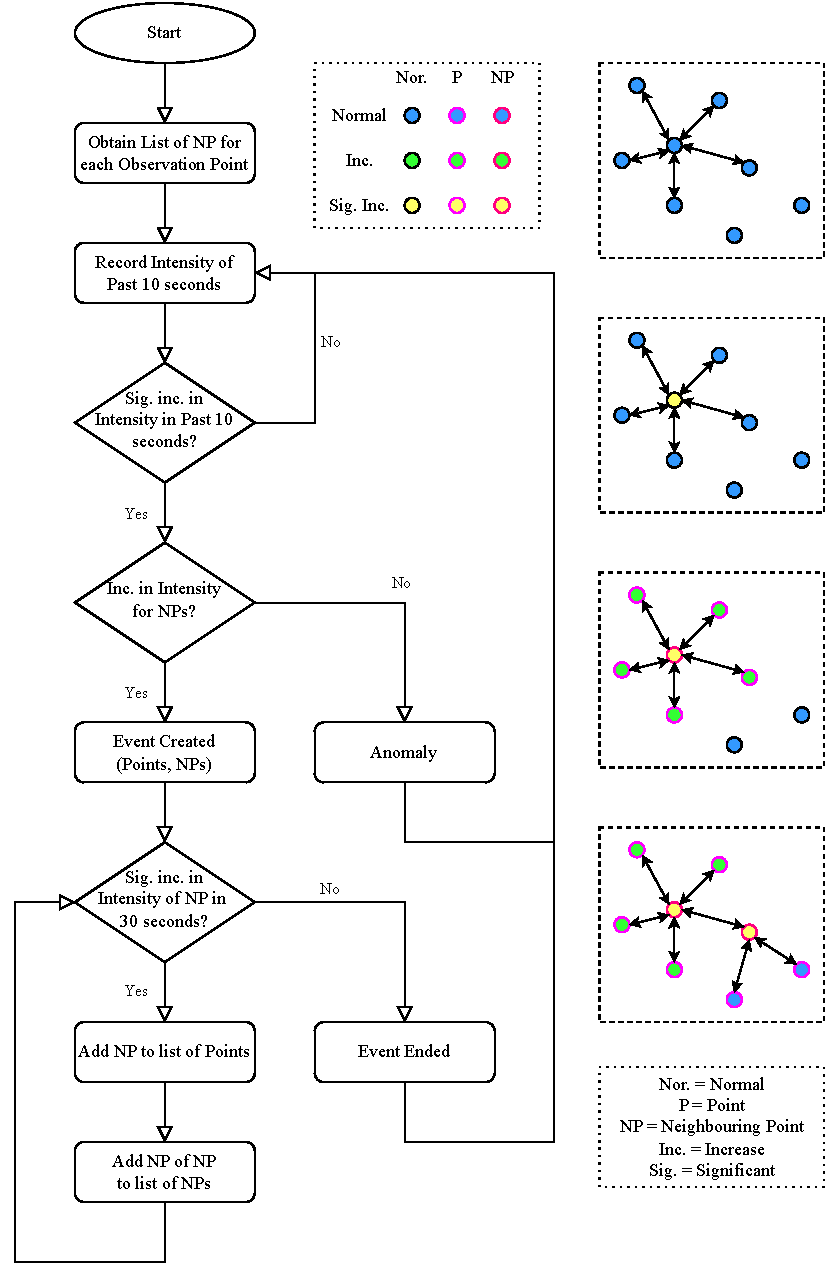
\includegraphics[width=0.8\linewidth]{shake-detection.pdf}
    \caption{Shake detection flowchart and diagram}
    \label{fig:shake-detection-diag}
\end{figure}

This section referred to \autocite{blog-ingen-shake-detection}.

\section{User Interface}

The GUI will be designed using Avalonia, which is designed to develop cross-platform applications in .NET.

The nature of this application decided that the UI will be a graphical interface. Comparing MAUI in .NET with Avalonia, due to the fact that MAUI is more suitable for a mobile touch-based platform (that also works on desktop), while Avalonia is designed to support the desktop paradigm, the latter will be used to implement the graphical interface.

As discussed in the previous sections, there are three main pages that the program will include: the page for real-time observations, the page for viewing past earthquakes, and the page for controls and settings.

A sidebar is used to switch between the three pages.

The mock-ups of GUI Pages are demonstrated using \autocite{soft-balsamiq}.

Note that the following mock-up images are for demonstration purposes only -- it is not an actual earthquake. They only include functionalities identified as 'key' in the analysis section, and therefore additional functionalities like shake-detection boxes, as well as customisation features are not included.

\subsection{Map}

The package Mapsui \autocite{mapsui-github} will be used to draw the maps in the application, since it is one of the best-supported candidates in .NET.

The OpenStreetMap layer will be used as the background, first because it is free to use and supported very well, also does it allow users to see the actual map of the area of which the earthquake occurred.

To colour the regions and the shorelines, Shape Files (\Code{.shp}) has to be used in the application. The Shape Files are sourced from the JMA webpage \autocite{jma-shapefiles}.

However, the shape files are extremely precise and accurate, tracing each and every coastline and border of the regions. However, this is not necessary for the purposes of the application (it does not make much difference zoomed out), and this will cause performance issues (loading the original shape files will cause a performance issue using more than 4 GB of RAM and will cause the application to halt).

Therefore, using the tool available on \autocite{soft-mapshaper}, the shape files are simplified using the Ramer--Douglas--Peucker algorithm, preserving 5\% of the original details (which is still extremely accurate), and the line intersections are also repaired (which is a natural consequence of the algorithm). However, this algorithm is not a key part to this application, so the existing implementation on \autocite{soft-mapshaper} is used.

\subsection{Real-Time Monitoring Screen}

The real-time monitoring screen holds the following three functionalities:
\begin{itemize}
    \item real-time intensity display;
    \item tsunami warning display (including shoreline colouring); and
    \item EEW display (including hypocentre marking, predicted intensity colouring and real-time wavefront positions).
\end{itemize}

\begin{figure}[htp]
    \centering
    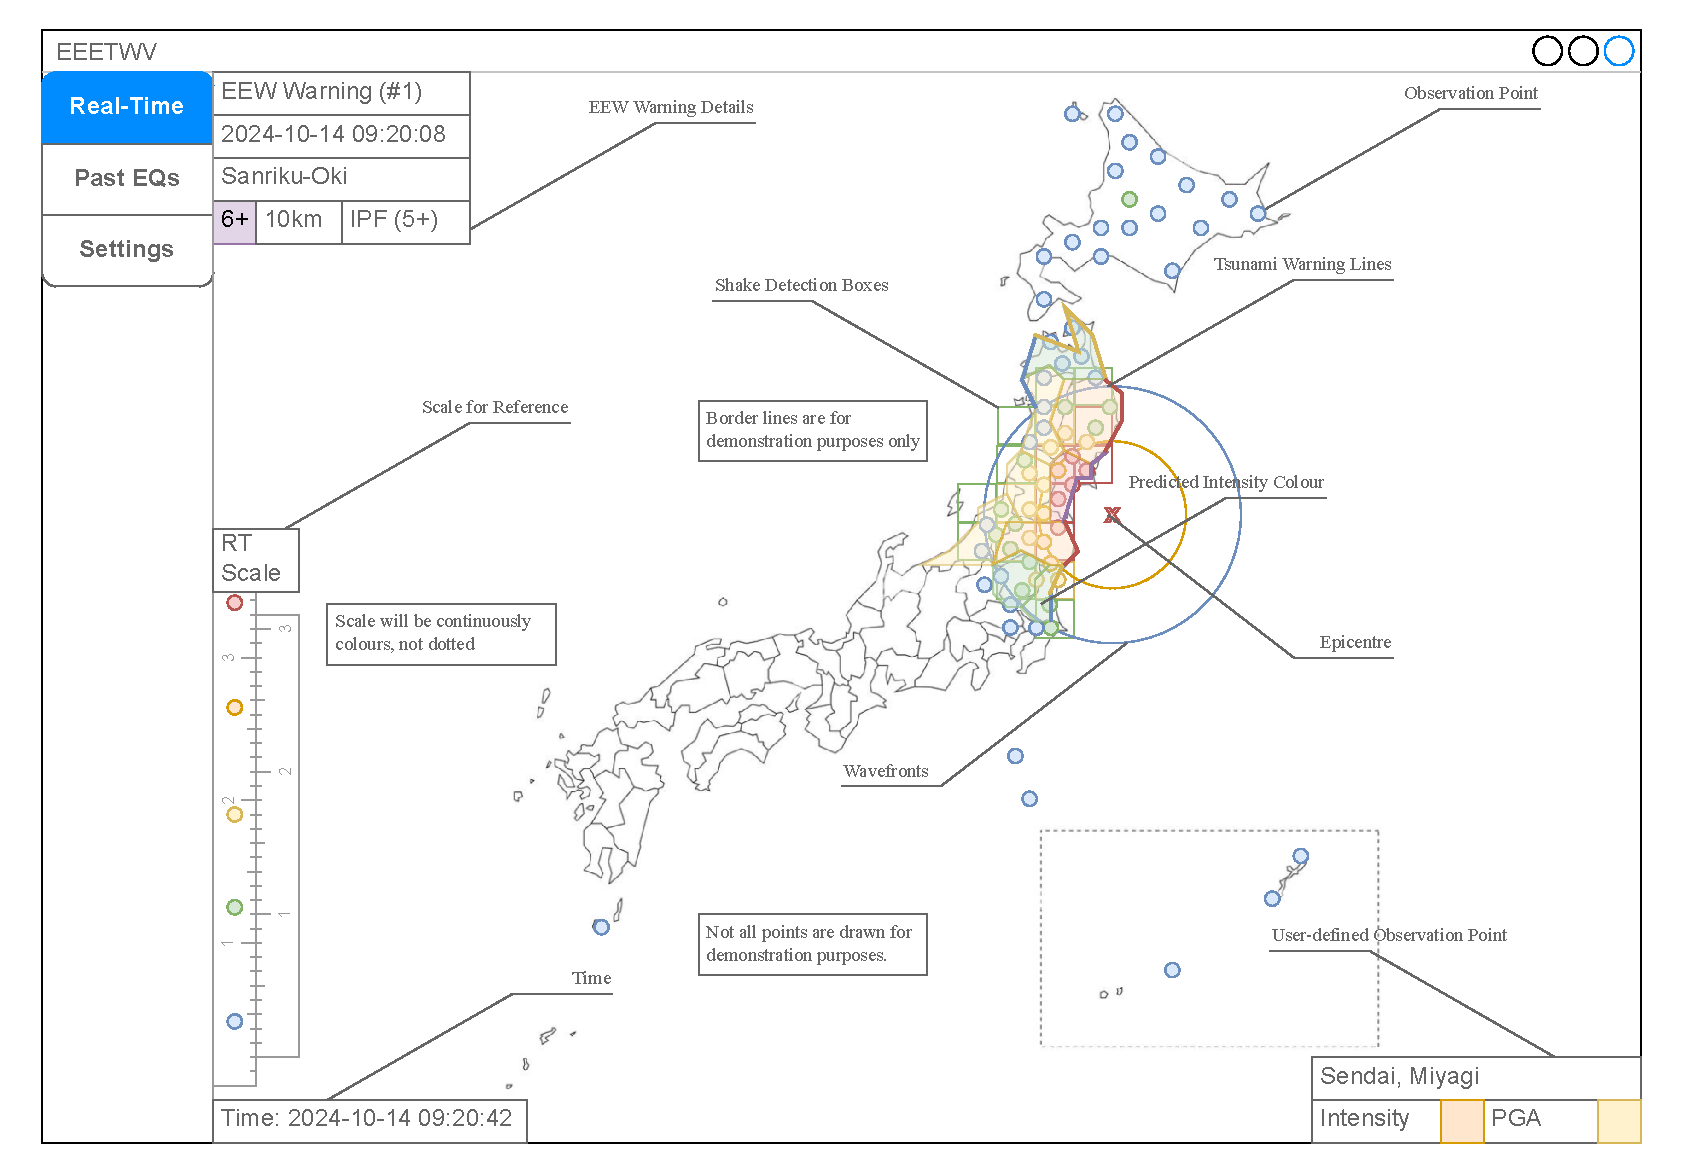
\includegraphics[width=\linewidth]{gui-mockup-rt.pdf}
    \caption{Design of GUI for Real-Time Page}
    \label{fig:gui-mockup-rt}
\end{figure}

Figure \ref{fig:gui-mockup-rt} shows a design of this page that should be implemented.

The real-time intensity colour points, the current time and the colour scale will be displayed at all times. On the colour scale, there will be the name of the current data displayed, with the number to indicate the scale of the colour. The colour scale and time are situated in the bottom-left corner of the page.

If a EEW is received, there will be a side panel appearing in the top-left corner of the screen. It should display the level of the EEW, together with the serial of the EEW. The level of the EEW has priority follows: Cancellation > Final > Warning > Forecast. The EEW will take level the first in the list that it is in. The details of the EEW are displayed, together with the informational text in scrollable form.

Upon receiving or updating an EEW, the hypocentre of the earthquake will be marked on the map. If the hypocentre is a seismological hypocentre, a red cross will be used. However, if the hypocentre is assumed and does not seismological meaning, as discussed in the analysis section, a different symbol will be used. The author chose to use a dashed circle.

The predicted maximum intensity of regions will also be coloured, and the wavefronts as well, with the P-Wave being blue (since less destructive) and S-Wave being orange (since more destructive).

If multiple EEWs are in effect simultaneously, then the top-left panel will switch between the earthquakes at a fixed rate. However, the information on the map for both earthquakes will be displayed simultaneously.

The EEW shall be removed (and the layers on the map as well) after a certain amount of time.

The tsunami warning will be displayed only if it is released, or updated. The shorelines will be coloured in accordance of the predicted warning level of the tsunami on that particular shore line region. In the bottom-right corner, the level of the tsunami warning (which is the maximum of the tsunami warnings for each shoreline) will be displayed including its colour, and the last update time. There will be a scrollable bar for the informational text, since it is usually very long.

There are no buttons for the user to interact with. However, there will be scroll bars for users to view the informational text for the particular earthquake, and the user will be able to zoom/move the map (as supported by Mapsui).

\subsection{Past Earthquakes}

The past-earthquake screen regularly displays a sidebar to select the earthquake from, with a map in the middle, and on the left a panel displaying the detailed information of the selected earthquake. Figure \ref{fig:gui-mockup-pe} shows a design of this page.

\begin{figure}[htp]
    \centering
    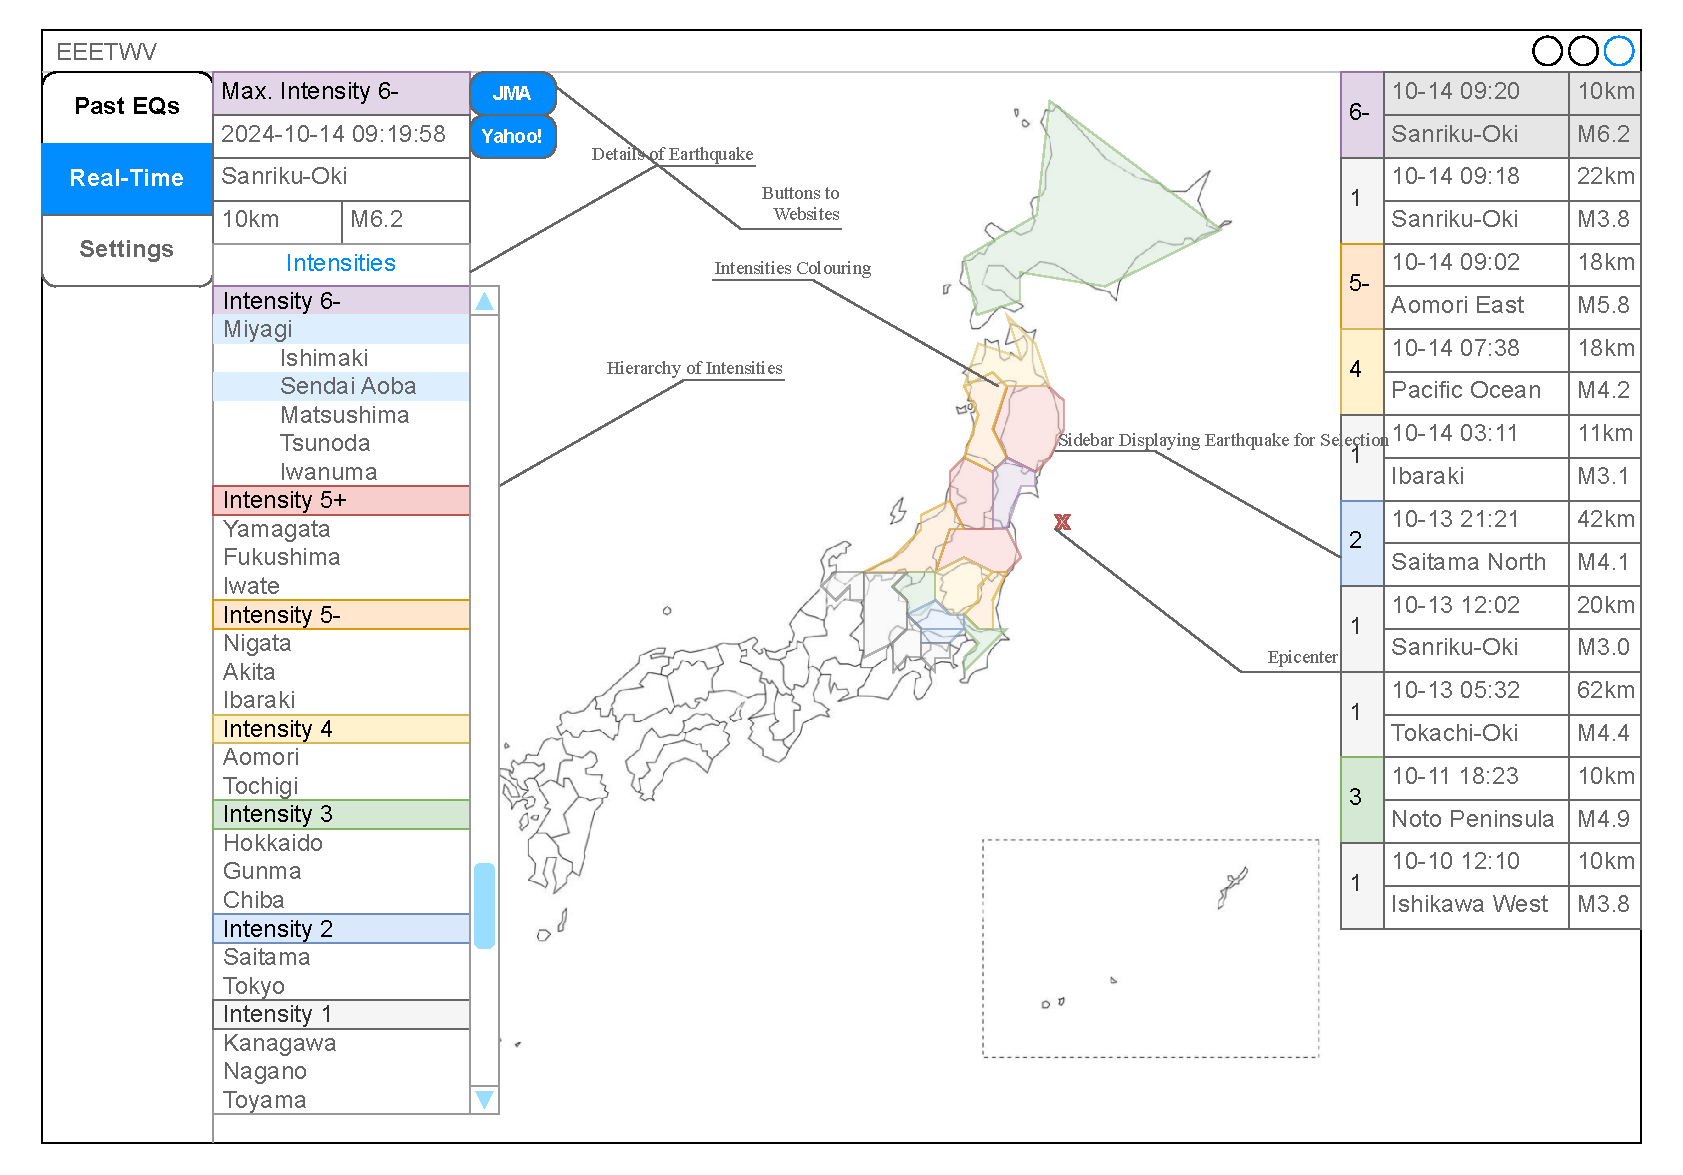
\includegraphics[width=\linewidth]{gui-mockup-pe.pdf}
    \caption{Design of GUI for Past Earthquakes Page}
    \label{fig:gui-mockup-pe}
\end{figure}

On the sidebar, for each earthquake, the intensity will be displayed, coloured as defined in the colour scheme. The name of the hypocentre's location, the depth, the magnitude, and the time of the earthquake is also included.

Notice that there are special cases of magnitudes, such as in different units, huge earthquakes or unknown, and special cases of depths as well, such as very deep, shallow or unknown.

Above the sidebar there is a load/refresh button, and below a button to load earthquakes. The sidebar is scrollable.

In the centre of the map, there is a red cross indicating the position of the hypocentre. Regions are coloured based on the maximum observed intensity in the region, and there are dots on the map indicating the observed intensity at that particular observation station.

On the left, the details of the selected earthquake will be displayed. On the top there is the button to link to Yahoo Earthquake Information. The information will be displayed more accurately here, together with the last updated time of the information. Then, there is the additional text and comments in scrollable form (since they could be quite long), and finally there is the intensity tree, first grouping by intensity, then by region, then by city, and finally the exact observation stations. The intensity level should be coloured in correspondence with the colour for that intensity.

The interactions the users is allowed to do on a page is to select an earthquake from the sidebar, and to click the load/refresh button to load the earthquakes. The user is also allowed to click on the Yahoo Earthquake Information button to view the information on the Yahoo Earthquake Information page. They are allowed to interact with the map (zoom/move), as well as using the scrollbars.

\subsection{Settings Page}

Figure \ref{fig:gui-mockup-se} shows a mock-up of the design of the customisation page.

\begin{figure}[htp]
    \centering
    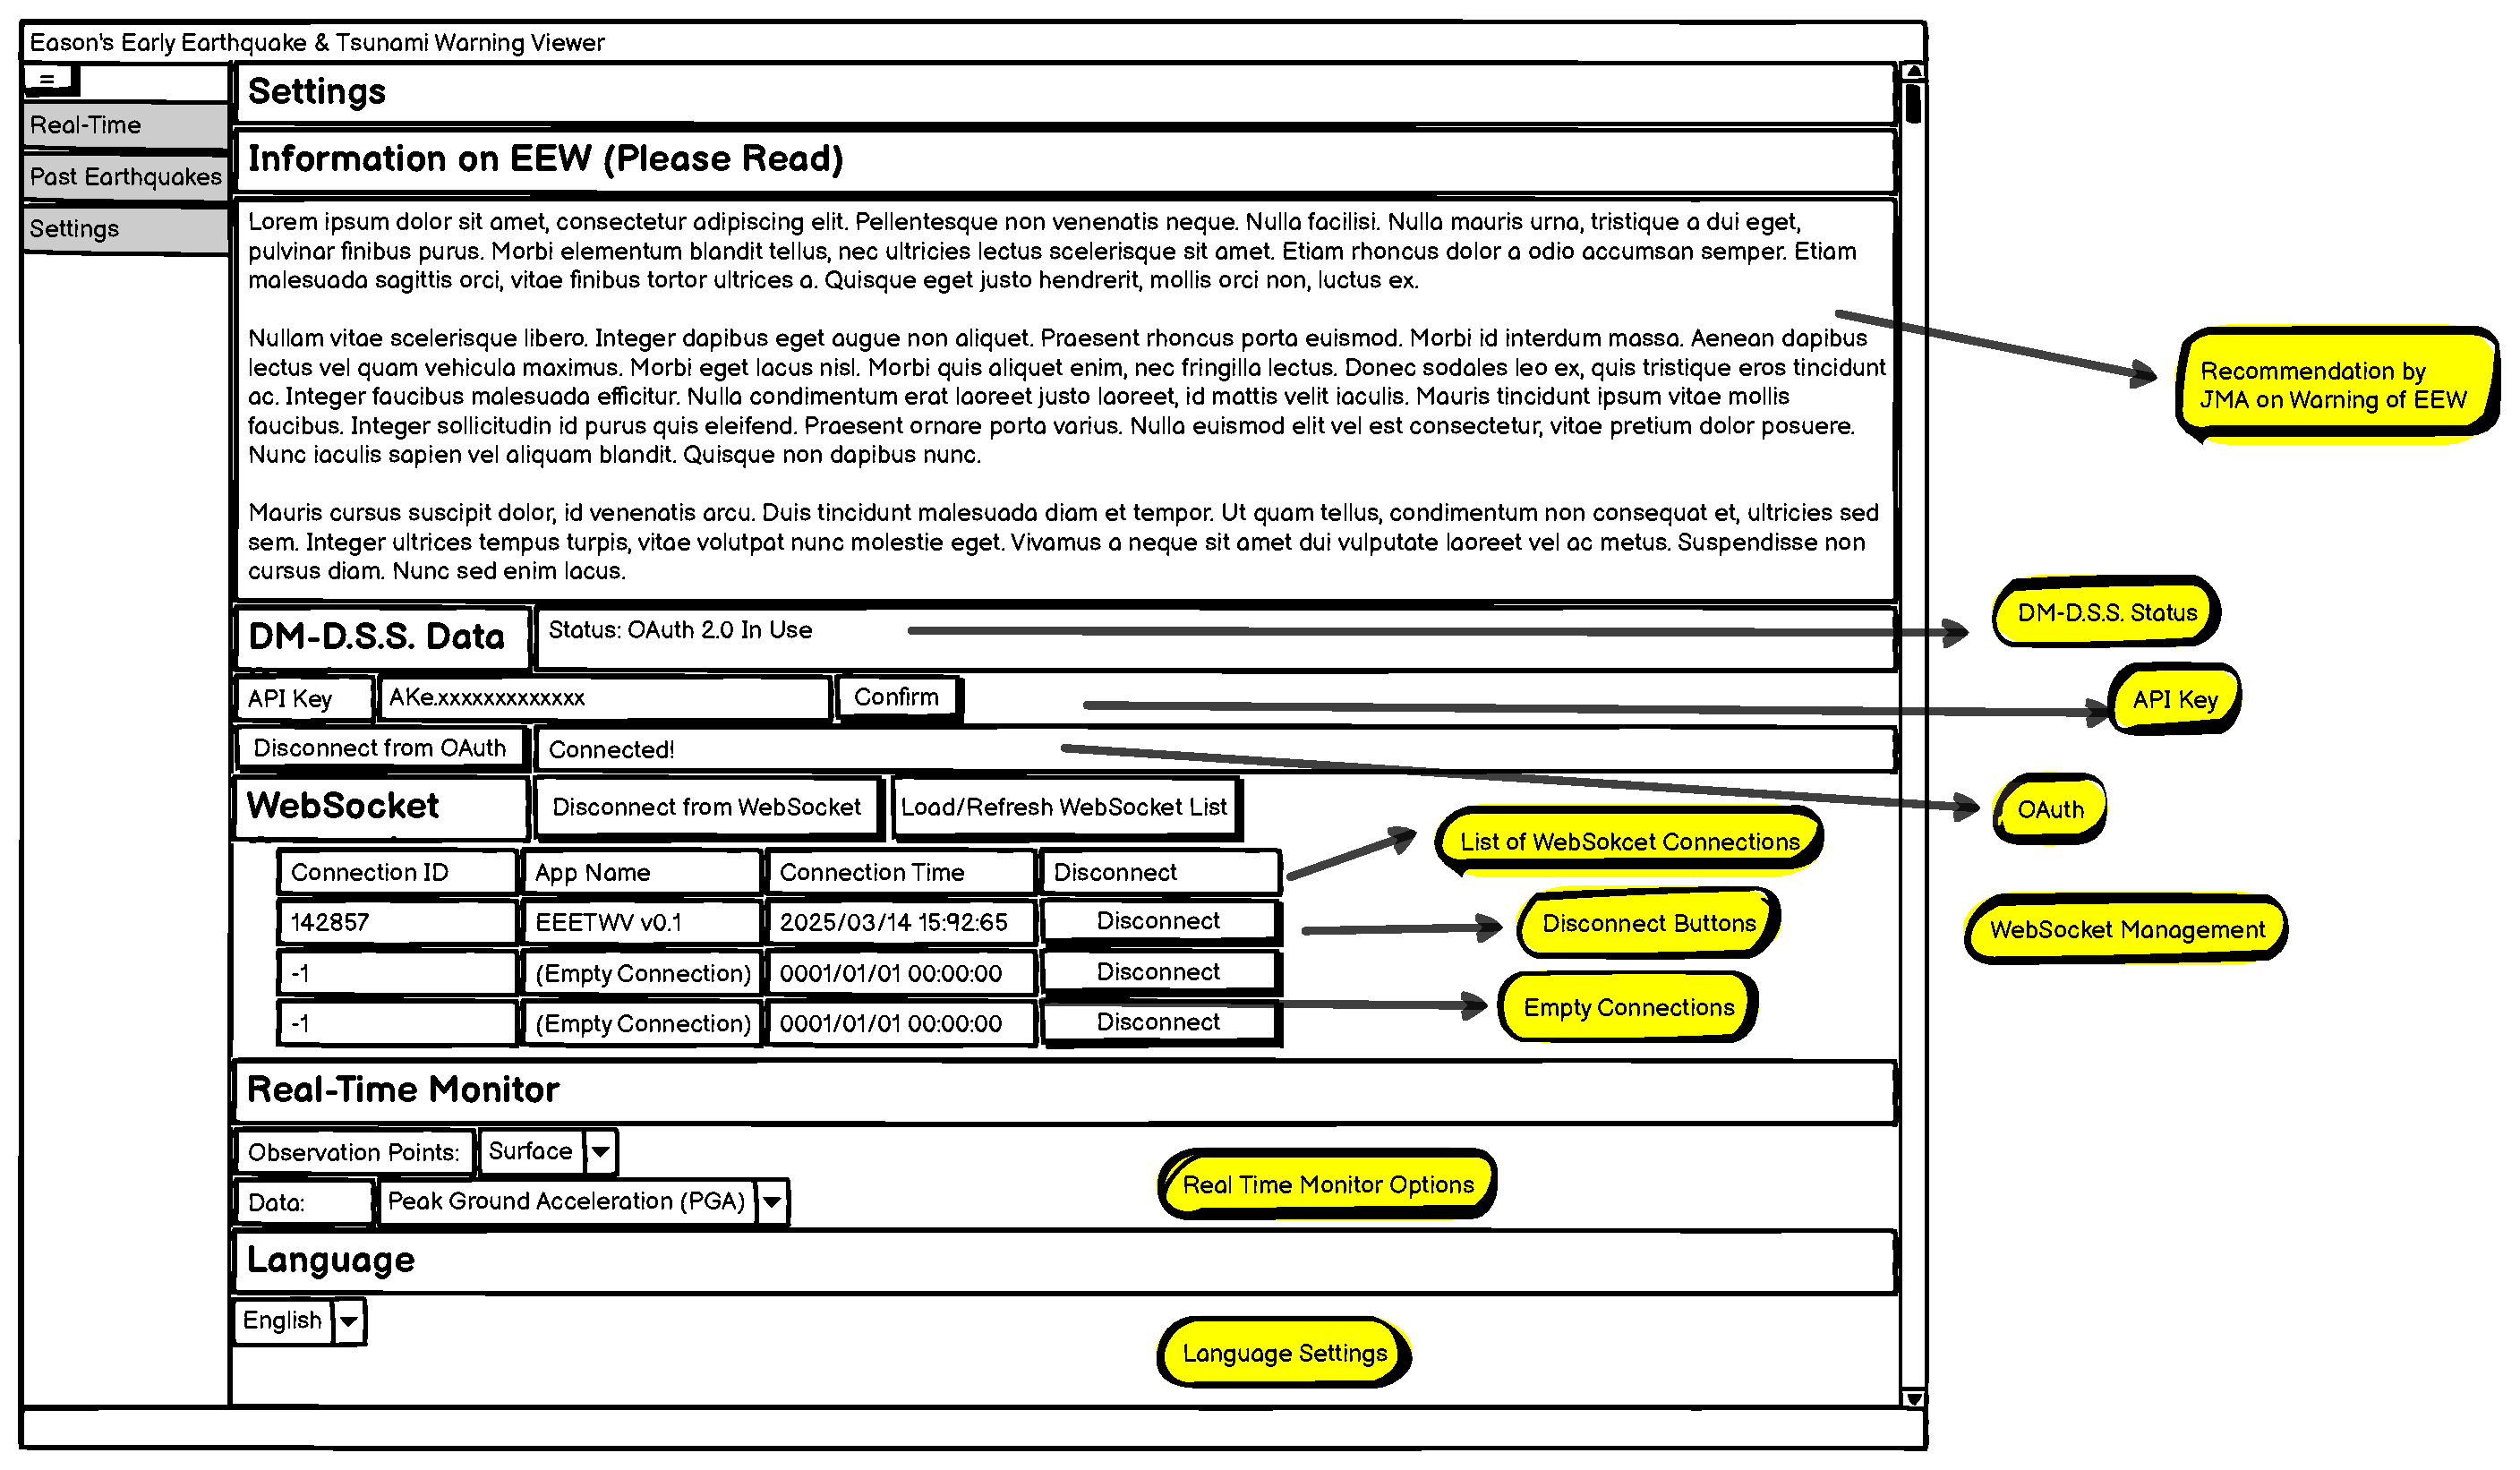
\includegraphics[width=\linewidth]{gui-mockup-se.pdf}
    \caption{Design of GUI for Settings Page}
    \label{fig:gui-mockup-se}
\end{figure}

In the settings page, according to the JMA requirements, there has to be explanatory text explaining the limitations and possible errors of EEWs.

There then should be a section to set up DM-D.S.S., where the user is allowed to enter an API Key and there should be a place to input an API Key from DM-D.S.S., or click a button to connect to OAuth 2.0.

Since OAuth 2.0 takes priority over API Key, the connect/disconnect button for OAuth is enabled all the time, allowing the user to authorise/revoke authorisation of the application.

The button to confirm the API Key should only be enabled if and only if all the following conditions are satisfied:
\begin{enumerate}
    \item The API Key input box has changed;
    \item The API Key has the correct format (begins with \Code{AKe.});
    \item OAuth 2.0 is not in use.
\end{enumerate}

Next up there is the section for the WebSocket, where a button is provided to connect to/disconnect from the WebSocket, and to load/refresh the list of WebSockets. In the list of WebSockets, the ID, App Name, and Connection Name of a connection is displayed, and a disconnect button is provided per line for each line, which will be disabled upon successful disconnection.

Finally, there are two dropdowns corresponding to the sensors and data of the real-time monitoring screen. The user should be able to select the sensors/data that they would like to view in the dropdown, and the data in the real-time page will reflect accordingly to the user's choice, including the text and the numbers on the scale.

At the end there is also a dropdown for the user to select the language of the application, which will change the language of the application, necessarily working upon restart.

\subsection{Joint Functionalities and Technicalities}

There is a joint functionality between the real-time page and the past earthquakes page, that is, when a new EEW/Tsunami Warning is released, the application should automatically jump to the real-time page to display the latest earthquake information to the user.

Since this a GUI-based application, there will be a significant use of asynchronous programming and events, which will be detailed later in the OOP section.

\section{OOP Model}

The program mainly uses the OOP (Object-Oriented Programming) paradigm, since it allows code object to be modelled like real-live objects. This is particularly useful in this application, since each service could be represented by an object (e.g. the API caller, the WebSocket connection), and each operation on it is modelled as a method.

This section will discuss some design patterns to use in the application, and will include class diagrams for modelling of services and DTOs.

\subsection{Design Patterns}

\subsubsection{Dependency Injection and Singleton Pattern}

\textbf{Dependency injection} is an extremely helpful tool dealing with complex classes with multiple dependencies to initialise. It would be a terrible idea for each class to instantiate the dependency themselves (e.g. the View Model for the Real-Time, Past, Setting Page instantiating their own services for API Calls, Authentications, Telegrams, etc., or the telegram fetcher and the WebSocket both each instantiating their own services to parse telegrams), since firstly it breaks the principle of single responsibility, and secondly it is performance-costly (the garbage collector has to collect garbage all the time, heap has to be assigned and de-assigned), and will lead to a lot of code duplication.

Dependency injection is achieved by sharing a \textbf{common container} of services, which .NET has a built-in \Code{IServiceCollection} with concrete implementation \Code{ServiceCollection}. The service container will deal with how to provide in the correct dependencies to the class that requires it. This avoids the need of complicated constructors in the code.

\textbf{Singleton pattern} is a pattern commonly used with dependency injection. Restricted to this application, \textbf{all services are registered as singletons}, meaning that there will only be \textbf{one} instance of each service in the application, and all services which depends on it, will \textbf{share this common instance}. Its lifetime will be managed by the container of the dependency injection (and we will not worry about it, it will get dealt with after the application stops).

The only exception to this rule is the loggers, since two loggers are involved, both implementing \Code{ILogger}: the debug logger (by Microsoft) and my custom file logger, having different concrete implementations to the same base interface. This means they are to be registered as \textbf{enumerable} in the logger builder.

This section referred to \autocite{dotnet-tutorial-dependency-injection}, introducing the basics of dependency injection and how to use dependency injection with the Microsoft packages.

\subsubsection{Logging}

\textbf{Logging} is essential to the application, since it allows the developer to see what is happening, and allows the developer to deal with bugs that are reported by the users. It allows for tracking of what is happening with the application at all times.

Microsoft has a built-in \Code{ILogger} and \Code{ILoggerProvider} service. \Code{ILogger} is the actual logger, and \Code{ILoggerProvider} is a provider (factory) of the logger.

When the application is debugging, the built-in .NET Debug Logger will be used, and the logs will be logger to the output in debug. However, when the application is in production, the custom file logger will be used, and the logs will be logged to a file (a \Code{StreamWriter} which is a file stream).

Logging is used in almost every service class of the application, unless the functionality is trivial, or any actions on the class is always visible.

This section referred to \autocite{dotnet-tutorial-logging} introducing the Microsoft \Code{ILogging} interface, and how to use it with dependency injection.

\subsubsection{Adaptor Pattern}

\textbf{Adaptor pattern} is about adapting one interface to another. Here, we will not detail in about the adaptor pattern involved between the results achieved from the API calls and the models that stores the data for the UI (this will be discussed later in the MVVM pattern).

The only two other adaptor patterns involved here, is the adaptor for logging for Avalonia and Mapsui.

Avalonia uses a very similar (but different) logging interface \Code{ILogSink} to log, however we used the more modern \Code{ILogSink} interface, and we will need to adapt the \Code{ILogger} to \Code{ILogSink}. This is achieved by an adaptor class \Code{AvaloniaToMicrosoftLoggingAdaptor}, which will implement the \Code{ILogSink} interface, and aggregate a \Code{ILogger}. The \Code{Log} method will be implemented to call the \Code{Log} method of the \Code{ILogger}, and \Code{IsEnabled} to call the \Code{IsEnabled} method of the \Code{ILogger} as well. The \Code{ILogger} provided to the adaptor class will be retrieved from the dependency injection container.

On the other hand, Mapsui uses a delegate (a callback function) to achieve logging. This is relatively simpler to achieve, since we could just attach to the \Code{Logger.LogDelegate} method of Mapsui the log delegate we want, in our case the \Code{ILogger.Log} method, where the \Code{ILogger} is retrieved from the dependency injection container.

This section referred to \autocite{mapsui-logging, avalonia-logging} on how logging is achieved in MapsUI and Avalonia.

\subsubsection{Options Pattern}

It is almost certainly a bad idea to hard-encode some configurations (especially strings) in different services, such as the location of the file for the JMA Time Table, the base URI of API Calls, and the location to store the authenticator. Therefore, a commonly-used approach in .NET is to use a file named \Code{appsettings.json}. The bad thing about this approach, is that it is not typed, and it is stored like a dictionary with strings as keys. Luckily, Microsoft has an Options Binding pattern, which allows us to bind sections of the configuration JSON file, to an options class, which could then be injected into the dependency injection container, and used by the services.

The options pattern is used for the configuration for the JMA Time Table (for the location of the file), the configuration for the DM-D.S.S. (for the base URIs, the OAuth 2 setup options, and the start post data for WebSocket), and the configuration for the Kmoni components (for the base URI, relative URI, and the file path to which the observation points are stored). Other options will not be type bound, but retrieved in a similar method as the string key dictionary as described before.

A small caveat here is that the options bound using type \Code{T} will be used as a \Code{IOptions<T>} in the dependency injection container, and the options will be retrieved using the \Code{Value} property of the \Code{IOptions<T>}.

This section referred to \autocite{dotnet-tutorial-configuration} on best practices in binding options and how to do this with dependency injection.

\subsubsection{Factory Pattern}

First, there is the \Code{FileLoggerProvider} (which is the provider for my custom file logger), which implements a \Code{ILoggerProvider} to be used in the logger builder in dependency injection. Rather than providing a constructor for the user to directly call, there is a create method in the provider to create an instance, and that is essentially what factory pattern is about.

Some constructors (setting-up) of the services involved is relatively complicated (e.g. involved the base API which is a string, hence cannot be dependency injected), and others might require setting up two classes which is quite complicated (e.g. in OAuth2 services, if a new service is being set-up, then two classes are involved, one is the one getting the authorisation code and the other involves refreshing the token; while if reading refresh token from a file only the latter is needed). In these cases, factory classes or methods will hide this complexity to the users.

These will be introduced in detail later.

\subsubsection{MVVM Pattern}

The MVVM (Model-View-View Model) pattern is a commonly-used pattern in UI design. The main reason it is used is for a clear separation of concerns -- the \textbf{view} describes the windows, and \textbf{binds} to certain properties in the \textbf{view model}, which is the model that the view binds to, and actual data is stored in the \textbf{models}.

As a brief description of the pattern, the following interfaces will be discussed. The detailed discussion of the view models and the models will be left to later.

\paragraph{\Code{INotifyPropertyChanged}}

This interface is the most commonly-used interface in MVVM -- it allows the object to notify other objects (that subscribes to it) whenever its properties has changed. It is especially useful in MVVM pattern, since it allows the model or the view model to notify the view model or the view that its properties to change, which allows the view model to deal with this accordingly, or let the GUI refresh the data of the view to update the window.

\Code{INotifyPropertyChanged} only defines one particular thing in the interface -- the \Code{PropertyChanged} event, which is an event that is raised whenever a property has changed.

This section referred to \autocite{avalonia-inotifypropertychanged}.

\paragraph{\Code{ObservableObject}, \Code{ObservableProperty} and \Code{RelayCommand}}

It would be painful to implement this interface for every single model/view model, since we would need to implement a backing (private) field, and a public property whose set property raises the \Code{PropertyChanged} event.

\Code{CommunityToolkit.Mvvm} addresses this problem by providing a base class (\Code{ObservableObject}) and source generators \Code{ObservableProperty} and \Code{RelayCommand} to mark as attributes to use on the fields or on the methods, to generate the properties or the commands, respectively. It reduces our workload of implementing the same interface for each property repeatedly, and is very useful in the MVVM pattern. We will use this significantly to implement the view models in the MVVM pattern.

This section referred to \autocite{dotnet-tutorial-mvvm-toolkit}.

\subsubsection{Reflection}

There are multiple enumerations that we would like to bind to in our view. Therefore, extension methods are provided to convert the enumerations to a readable string, or to a colour string, to bind to the view. However, the implementation of the Avalonia binding system decided that binding will not be possible with the extension methods.

Therefore, \textbf{converters} are used here. Specifically, the typed one-way converter \Code{FuncValueConverter} is used. However, it would be ridiculous to write such a converter for each enumeration.

Therefore, the code is designed to put all extension methods for converting to a string in a single class, and all extension methods for converting to a colour in another class.

A converter is then written for the generic \Code{Enum} class to convert to a string. Then, \textbf{reflection} will be used to find the list of all the methods provided by the particular extension classes, and filtering the method that takes the specific concrete type of the enumeration as the parameter, and invoke the method on it to convert to string. This is still type-safe, since the type check for parameters is used, but we have achieved 'type-safe dynamic typing' using reflection!

This section referred to \autocite{avalonia-custom-converter,dotnet-reference-getmethods, dotnet-reference-getmethods, dotnet-reference-bindingflags}.

\subsubsection{Events}

\textbf{Events} are raised when something of interest happened, and a \textbf{handler} is attached to the event to handle the event (i.e. executes some code). As an example, there are two events for WebSocket, the data received (which invokes the event handler in the real time view model), and status changed (which invokes the event handler in the setting view model).

The detailed use of events will be introduced in the separate components.

This section referred to \autocite{dotnet-tutorial-events}, the .NET guidance on how to raise and handle events.

\subsubsection{Exceptions}

Exceptions are thrown when unexpected things (errors) happen in the application code (e.g. when an API call fails, when a WebSocket disconnects unexpectedly, when an attempt to write to a file fails). Exceptions are to be \textbf{handled} by the application (and should not cause the application to crash any way) and logged into the logs.

Custom exceptions are designed in the authentication, telegram, and WebSocket components in the application, and will be demonstrated later within the class diagrams.

This section referred to \autocite{dotnet-tutorial-exception}, the .NET guidance on how to create custom exceptions, and best practices on handling exceptions.

\subsection{Abstractions (Interfaces), Options and Services (Classes)}

Interfaces is an abstraction of a service, and is a contract between the service and the user on what the service will be able to do. It defines the functionality of the service, but does not provide the implementation. This is especially useful for mocking the service for unit testing purposes, and provide the possibility for polymorphism, which could be achieved by different implementation of the same service.

Options on the other hand gives the service the necessary setup data. In most cases, it makes the constructor more meaningful, and allows for the options pattern and binding to an external settings file (see later for a detailed description of the settings pattern).

Each section below is the description of one particular responsibility (service) that is necessary for the application, and in separate namespaces.

\subsubsection{JMA Time Table}

For the service of the JMA Time Table, \textbf{options pattern} is used to provide the location of the raw text file (the only setup required).

\textbf{Abstraction} is provided for the service that calculates the distance based on the time and depth, and this is the only responsibility of the interface, \Code{ITimeTable}.

The services will be split into two parts: the actual service for the Time Table, \Code{TimeTable}, and the builder of the Time Table Database, \Code{TimeTableBuilder}, which is responsible for reading the file, verifying that it has the correct format via the Regular Expression, and parsing the raw text file into the DTO format to be transferred into the Time Table service provider. This is an example of the \textbf{factory pattern}, and it will return an object with the type of the interface, rather than the concrete class itself. This hides the detail implementation from the user, and provides the user with only an interface to interact with.

Logging will be provided for the service class \Code{TimeTable}.

Extension methods on \Code{IServiceCollection} is provided to \textbf{inject} a singleton of \Code{ITimeTable} into the service collection, and the options pattern is used to provide the location of the file. This also hides the factory from the user as well.

This functionality does not have any dependencies on other functionalities.

Figure \ref{fig:class-diagram-timetable} is the class diagram for this functionality.

\begin{figure}[htp]
    \centering
    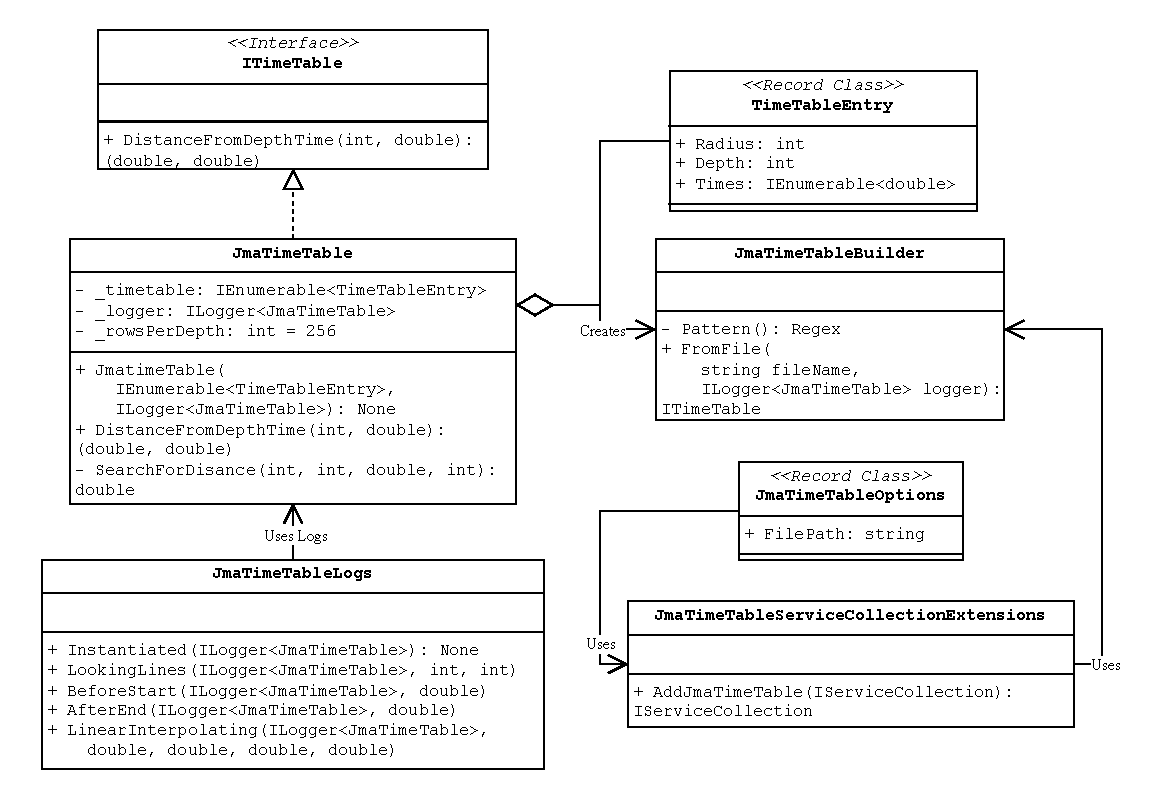
\includegraphics[width=\linewidth]{class-diagram-timetable.pdf}
    \caption{Class Diagram for JMA Time Table}
    \label{fig:class-diagram-timetable}
\end{figure}

\subsubsection{Kyoshin Monitor}

To manipulate with colours and images, the C\# library SkiaSharp is used, specifically the classes \Code{SKColor}, \Code{SKBitmap} and \Code{SKImage}.

The functionality is split into two parts, the fetching of the images from the webpage, and the extraction of the points using give data on the extraction of points in JSON format. As for the first functionality, the \textbf{abstraction} used is the interface \Code{IImageFetch}, and \Code{ImageFetch} is the concrete implementation of it. They all depend on two enumerations, the \Code{MeasurementType} and the \Code{SensorType}, with an extension class providing conversion of the enumerations to a string in the URI. \textbf{Logging} is achieved by \Code{ImageFetchLogs}.

The second functionality is the extraction of the points from the JSON data, and the \textbf{abstraction} used is the interface \Code{IPointExtraction}, and \Code{PointExtraction} is the concrete implementation of it.

For the DTOs to deserialise the JSON file which stores the mapping information of pixel position and geographical location, the DTO \Code{ObservationPoint} is used, \textbf{composed} in the class \Code{PointExtract} (i.e. they have the same life-cycle). \Code{GeographicCoordinate}, \Code{PixelCoordinate} and the enumeration \Code{PointType} has composition relationship with the \Code{ObservationPoint} class as well, since they are considered part of the observation point.

To achieve \textbf{dependency injection}, extension methods on \Code{IServiceCollection} is provided to inject \Code{IImageFetch} and \Code{IPointExtract} into the service collection, using \textbf{options pattern} to set up the base URI, relative URI format string, and the file path to the JSON file storing the mapping of pixels to geographical locations.

This functionality does not have any dependencies on other functionalities.

Figure \ref{fig:class-diagram-kmoni} is the class diagram for this functionality.

\begin{figure}[htp]
    \centering
    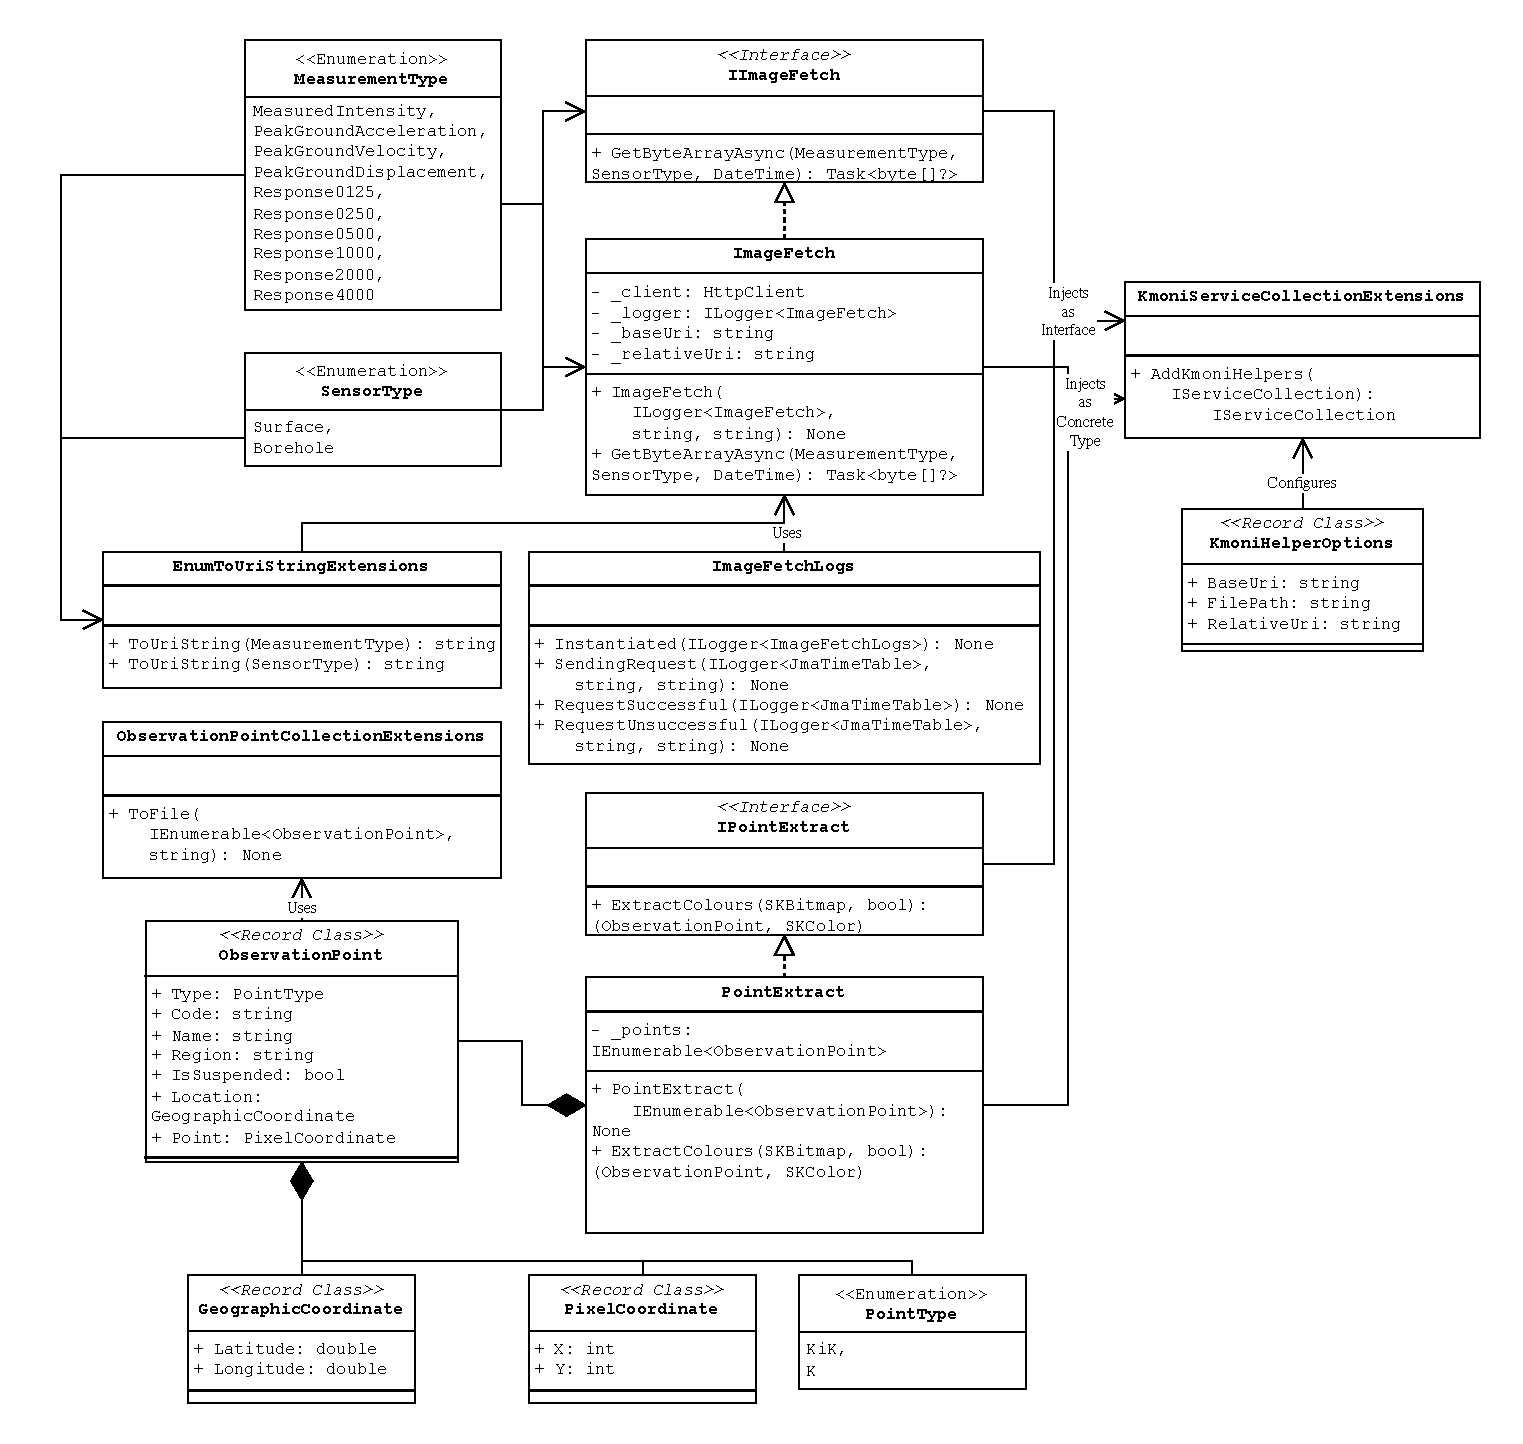
\includegraphics[width=\linewidth]{class-diagram-kmoni.pdf}
    \caption{Class Diagram for Kmoni}
    \label{fig:class-diagram-kmoni}
\end{figure}

Apart from those basic services, the colour conversion is included as extension methods provided in a static class. Also, an extension method is used in the conversion from the \Code{byte[]} to \Code{SKBitmap} to connect between \Code{IImageFetch} and \Code{IPointExtraction}. Figure \ref{fig:class-diagram-kmoni-extra} gives the class diagram for these two Functionalities.

\begin{figure}[htp]
    \centering
    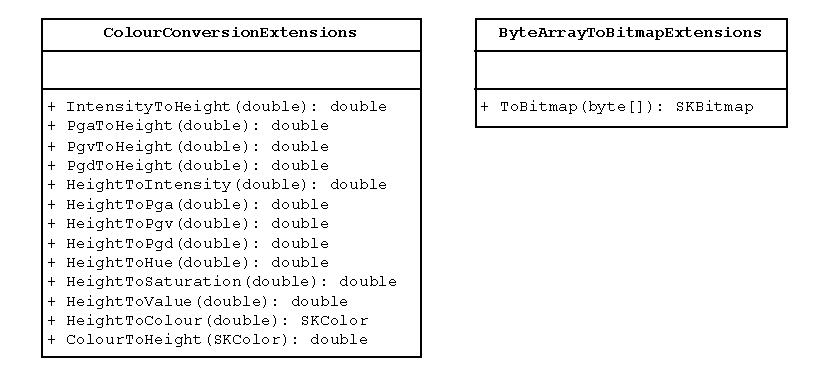
\includegraphics[width=0.75\linewidth]{class-diagram-kmoni-extra.pdf}
    \caption{Class Diagram for Extra Services of Kmoni}
    \label{fig:class-diagram-kmoni-extra}
\end{figure}

\subsubsection{DM-D.S.S. Authentication}

As briefly discussed previously, there will be three types of authenticators involved here: not authenticated (null authenticator), API key authenticator, and OAuth 2 authenticator. To \textbf{abstract} their behaviour, the interface \Code{IAuthenticator} is introduced. To manage the authenticators (to achieve a singleton pattern), the manager which acts as a \textbf{factory} is abstracted as \Code{IAuthenticatorHelper}. The enumeration \Code{AuthenticationStatus} is introduced to get the status of the current authenticator.

In terms of the concrete implementations of the interface, \Code{NullAuthenticator} is the easiest. It will throw a custom exception \Code{NullAuthenticatorException} when attempting to get a header from the class. However, since its behaviour is identical, it will be meaningless to create a new instance of it/dispose it when its necessary/unnecessary. Therefore, a common shared static instance is used, as in the \Code{Instance} property of the class. The \Code{ApiKeyAuthenticator} class also has a very simple implementation. It only has one thing, the API Key.

The OAuth 2 classes are slightly more convoluted. \Code{OAuth2Authenticator} is the key part of the functionality, and it implements \Code{IAuthenticator}. However, it is only its responsibility to acquire access token from refresh token, and to revoke tokens. The responsibilities of acquiring an authorisation code and the first refresh token is done by the \Code{OAuth2Helper} class, which shows a clear separate of concern. Since there are multiple parameters necessary to set up OAuth2, the \textbf{options pattern} is used and \Code{OAuth2Options} class provide the configuration. To hide this complexity, \textbf{factory methods} are also used, as in \Code{OAuth2Provider}. (Shared static methods between OAuth 2 classes are in \Code{OAuth2SharedMethod}).

Very simple DTO objects are used to store the JSON objects returned from the authentication endpoint. The \Code{Error} DTO class represents an error response, \Code{TokenRefresh} represents a token refresh response, and \Code{TokenRequest} represents a token request response. However, since \Code{TokenRequest} response is just basically \Code{TokenRefresh} response plus the refresh token, \textbf{inheritance} is used here to reduce redundant code.

All concrete implementations of \Code{IAuthenticator} must override the \Code{ToString} method to provide means of saving the authenticator to a file.

The concrete implementation of \Code{IAuthenticatorHelper} is \Code{AuthennticatorHelper}. It is responsible for creating the authenticator based the new choice of the authenticator (null, API Key, OAuth), and a method is also provided to read and setup from the string representation of the current authenticator from a file.

Furthermore, there is an \textbf{event} in \Code{IAuthenticatorHelper} which is \Code{AuthennticatonStatusChanged}, which notifies other parts of the code that it has changed. The refresh of the components of GUI Setting Page is achieved by subscribing to this event (adding event handler), and the writing of the current authenticator used to a file is also achieved this way (rather than hard-coding into the code, since that would break single-responsibility).

Extension methods are provided in \Code{AuthenticationHelperServiceCollectionExtension} to inject services into the dependency injection container. Logging is provided for \Code{AuthenticationHelper}, \Code{OAuth2Authenticator} and \Code{OAuth2Helper}, since they have quite convoluted functionalities.

Figure \ref{fig:class-diagram-dmdata-auth} gives the class diagram for this functionality.

\begin{figure}[htp]
    \centering
    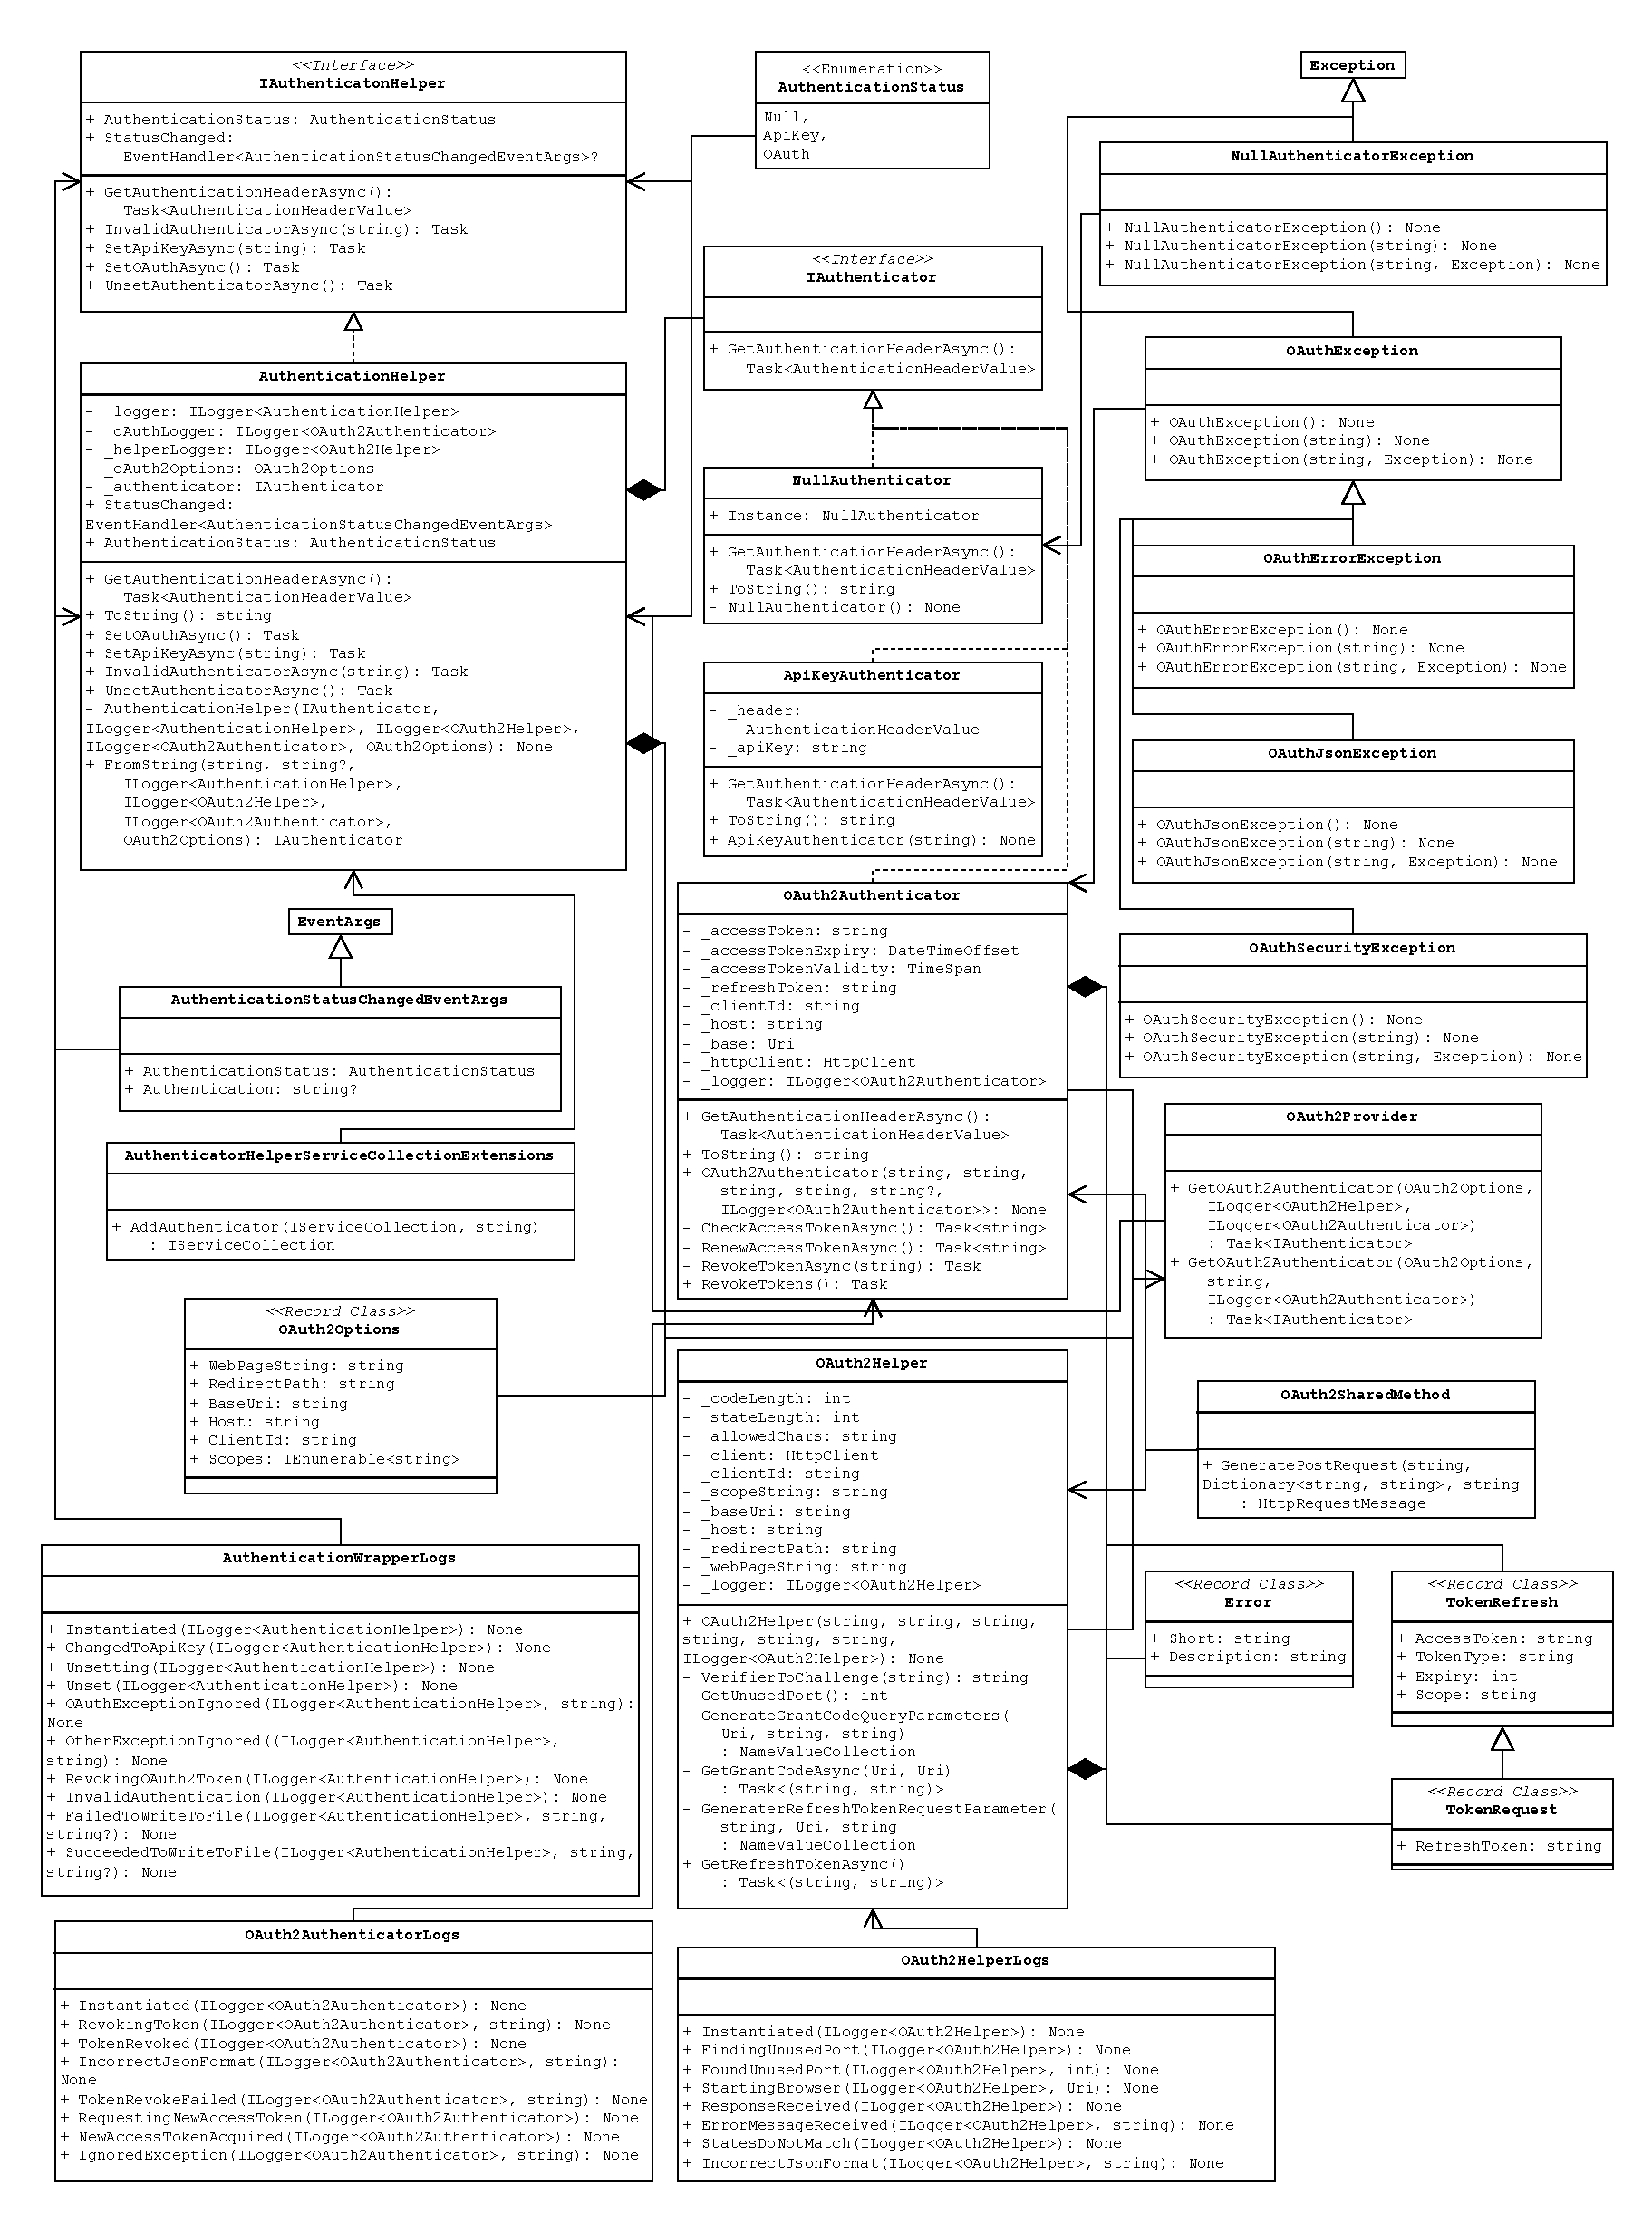
\includegraphics[width=\linewidth]{class-diagram-dmdata-auth.pdf}
    \caption{Class Diagram for DM-D.S.S. Authentication}
    \label{fig:class-diagram-dmdata-auth}
\end{figure}

\subsubsection{DM-D.S.S. API Calls}

The service for API calls is relatively trivial, with \Code{IApiCaller} representing the \textbf{abstraction}, \Code{ApiCaller} being the \textbf{concrete implementation}, and \Code{ApiCallerLogs} providing the \textbf{logs} for API calls. Extension methods for \textbf{dependency injection} are provided in \Code{ApiCallerServiceCollectionExtensions}, and some other service extensions are provided.

To improve code reusability (and share error-handling code and behaviour), there are several private methods introduced in \Code{ApiCaller} for this. For example, \Code{CreateHttpRequest} is used to create HTTP Requests, \Code{HandleError} is used to handle errors in HTTP Requests, and \Code{SendRequestAsync} is used to send requests.

Notice that this class should not expose API errors to the external code that is using it -- it will just return null if the API call fails.

The class diagram is in Figure \ref{fig:class-diagram-dmdata-api}. Notice that this does not include the DTOs, since they are not part of the service. (They will be discussed later.)

\begin{figure}[htp]
    \centering
    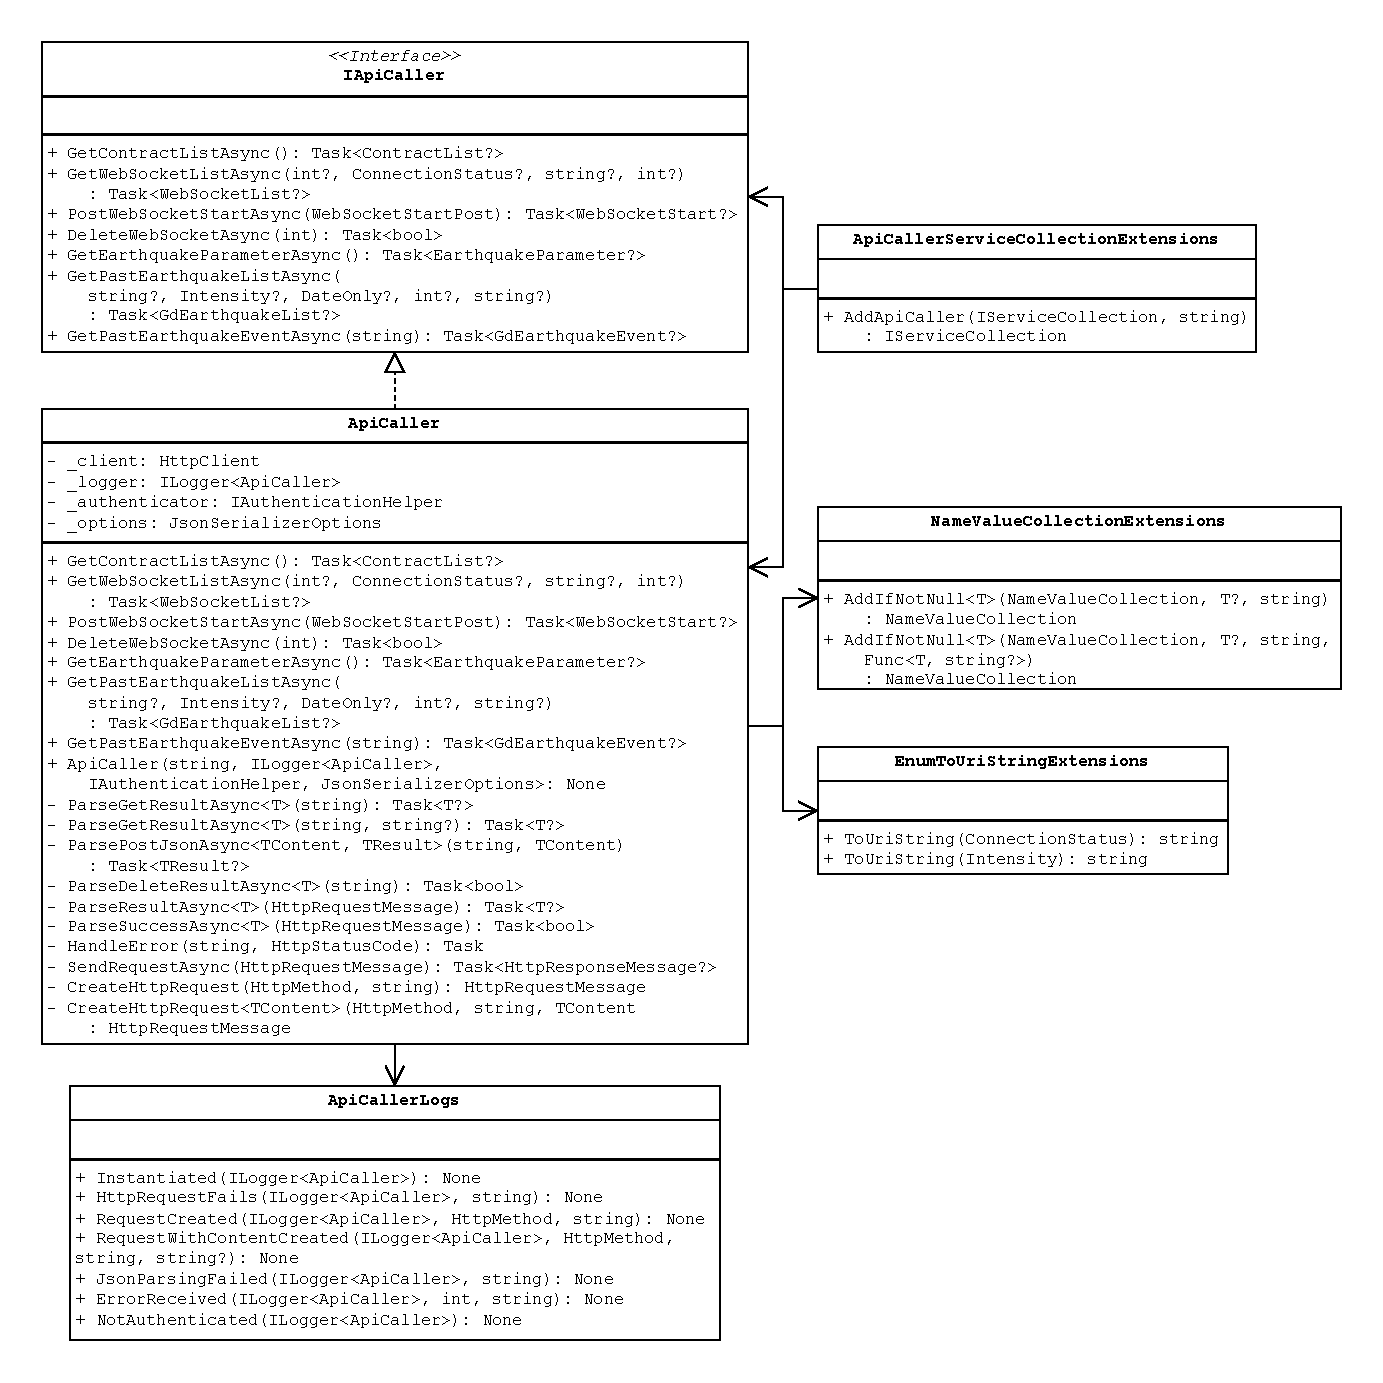
\includegraphics[width=\linewidth]{class-diagram-dmdata-api.pdf}
    \caption{Class Diagram for DM-D.S.S. API Calls}
    \label{fig:class-diagram-dmdata-api}
\end{figure}

This service depends on the authentication service, and the common DTOs.

\subsubsection{DM-D.S.S. Telegram Fetching and Parsing}

The responsibilities of parsing the schema for the JSON telegram and parsing the telegram, is separate responsibilities from fetching the JSON telegram. Therefore, there are two \textbf{interfaces} involved here: \Code{ITelegramParser} for parsing the JSON into the DTO of the corresponding schema, and determining the C\# type of the object corresponding to a schema; and \Code{ITelegramRetriever} for acquiring the telegram itself from the API.

Their concrete services are \Code{TelegramParser} and \Code{TelegramRetriever} respectively. However, notice that \Code{TelegramRetriever} would aggregate an object of \Code{TelegramParser}. This is an \textbf{aggregation} since their life cycle are not fully (though highly) correlated -- the parser is provided in the constructor for the retriever, and could as well exist without the retriever.

Both concrete services have \textbf{logging}, and extension methods for \textbf{dependency injection} is also provided. Similar to previous classes, due to the existence of the dependency injection methods, the service classes are not exposed to external code, and the only way to create an instance of the service is through the dependency injection container.

The class diagram is in Figure \ref{fig:class-diagram-dmdata-telegram}.

\begin{figure}[htp]
    \centering
    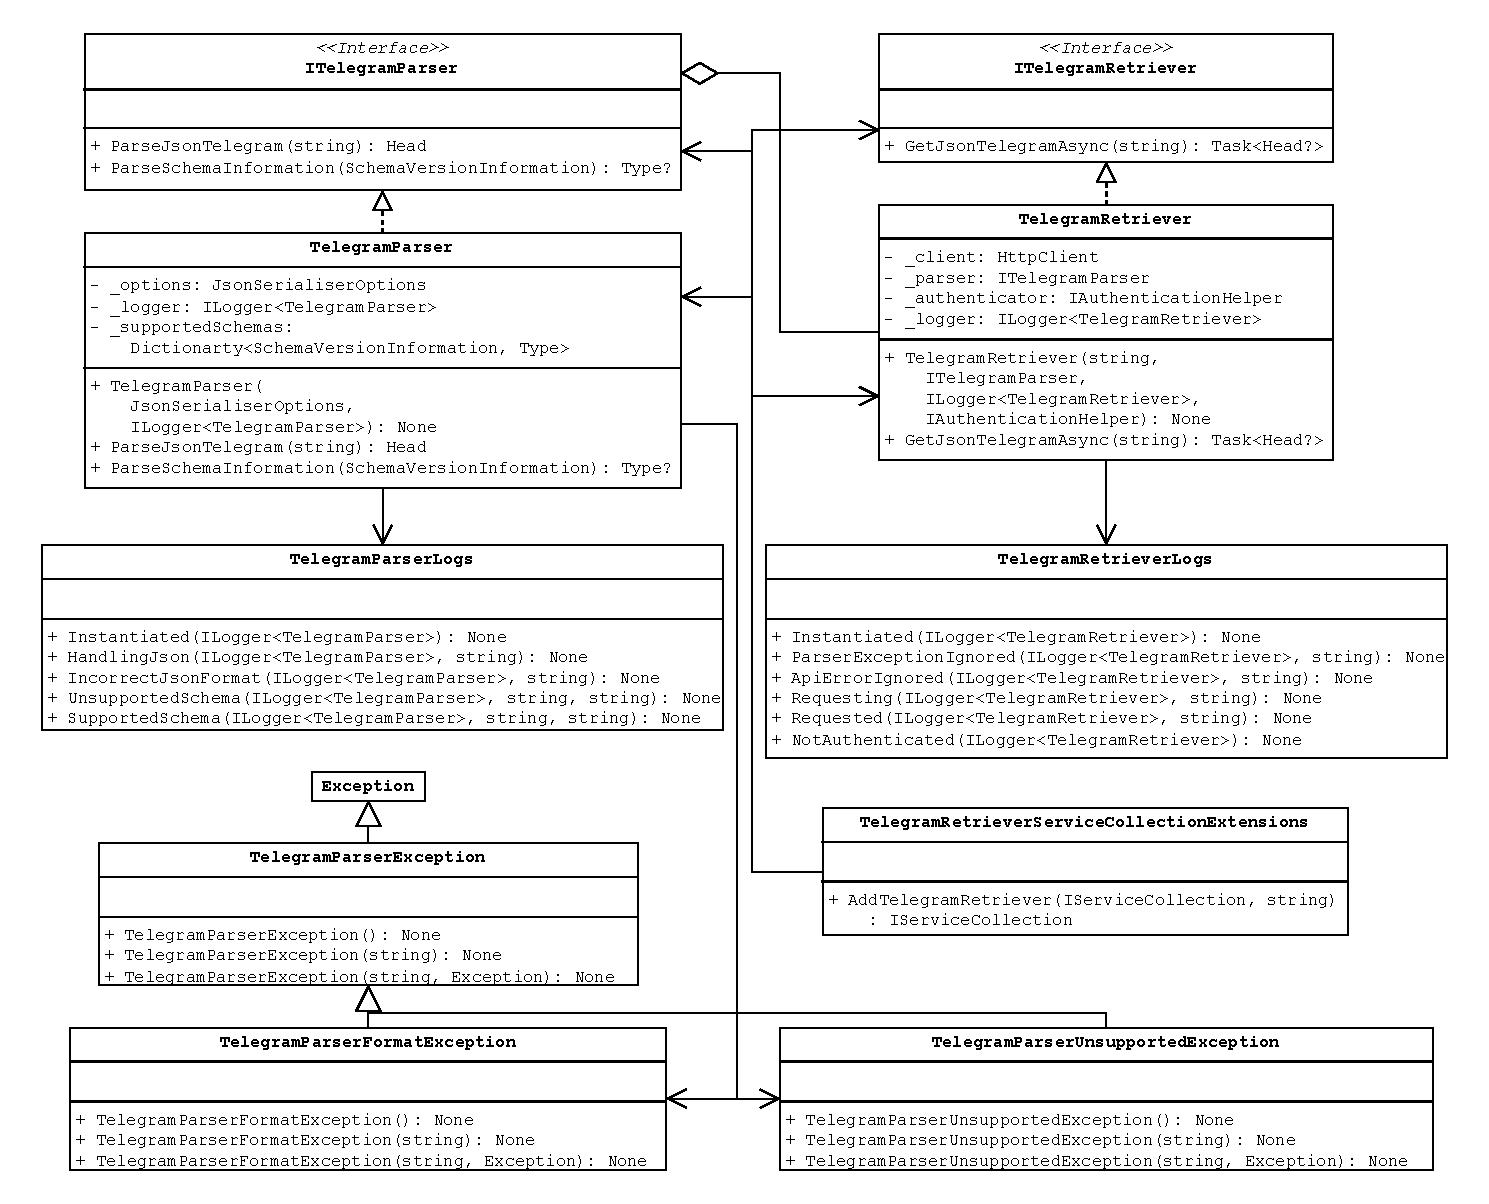
\includegraphics[width=\linewidth]{class-diagram-dmdata-telegram.pdf}
    \caption{Class Diagram for DM-D.S.S Telegram Fetching and Parsing}
    \label{fig:class-diagram-dmdata-telegram}
\end{figure}

This component has dependency on the authentication class, and the shared common DTOs.

\subsubsection{DM-D.S.S. WebSocket}

There is one \textbf{interface} for this, \Code{IWebSocketClient}, and the concrete \textbf{service} is \Code{WebSocketClient}.

There are two events: data received (with event arguments \Code{DataReceivedEventArgs}, containing the telegram received), and status changed (with event arguments \Code{StatusChangedEventArgs}, containing a boolean indicating if the new connection is connected). \textbf{Exceptions} are designed as well, but this is mainly for internal purposes, and they will not be exposed to the users of this (all handled internally).

The class diagram is in Figure \ref{fig:class-diagram-dmdata-ws}. Note that DTOs are excluded from this.

\begin{figure}[htp]
    \centering
    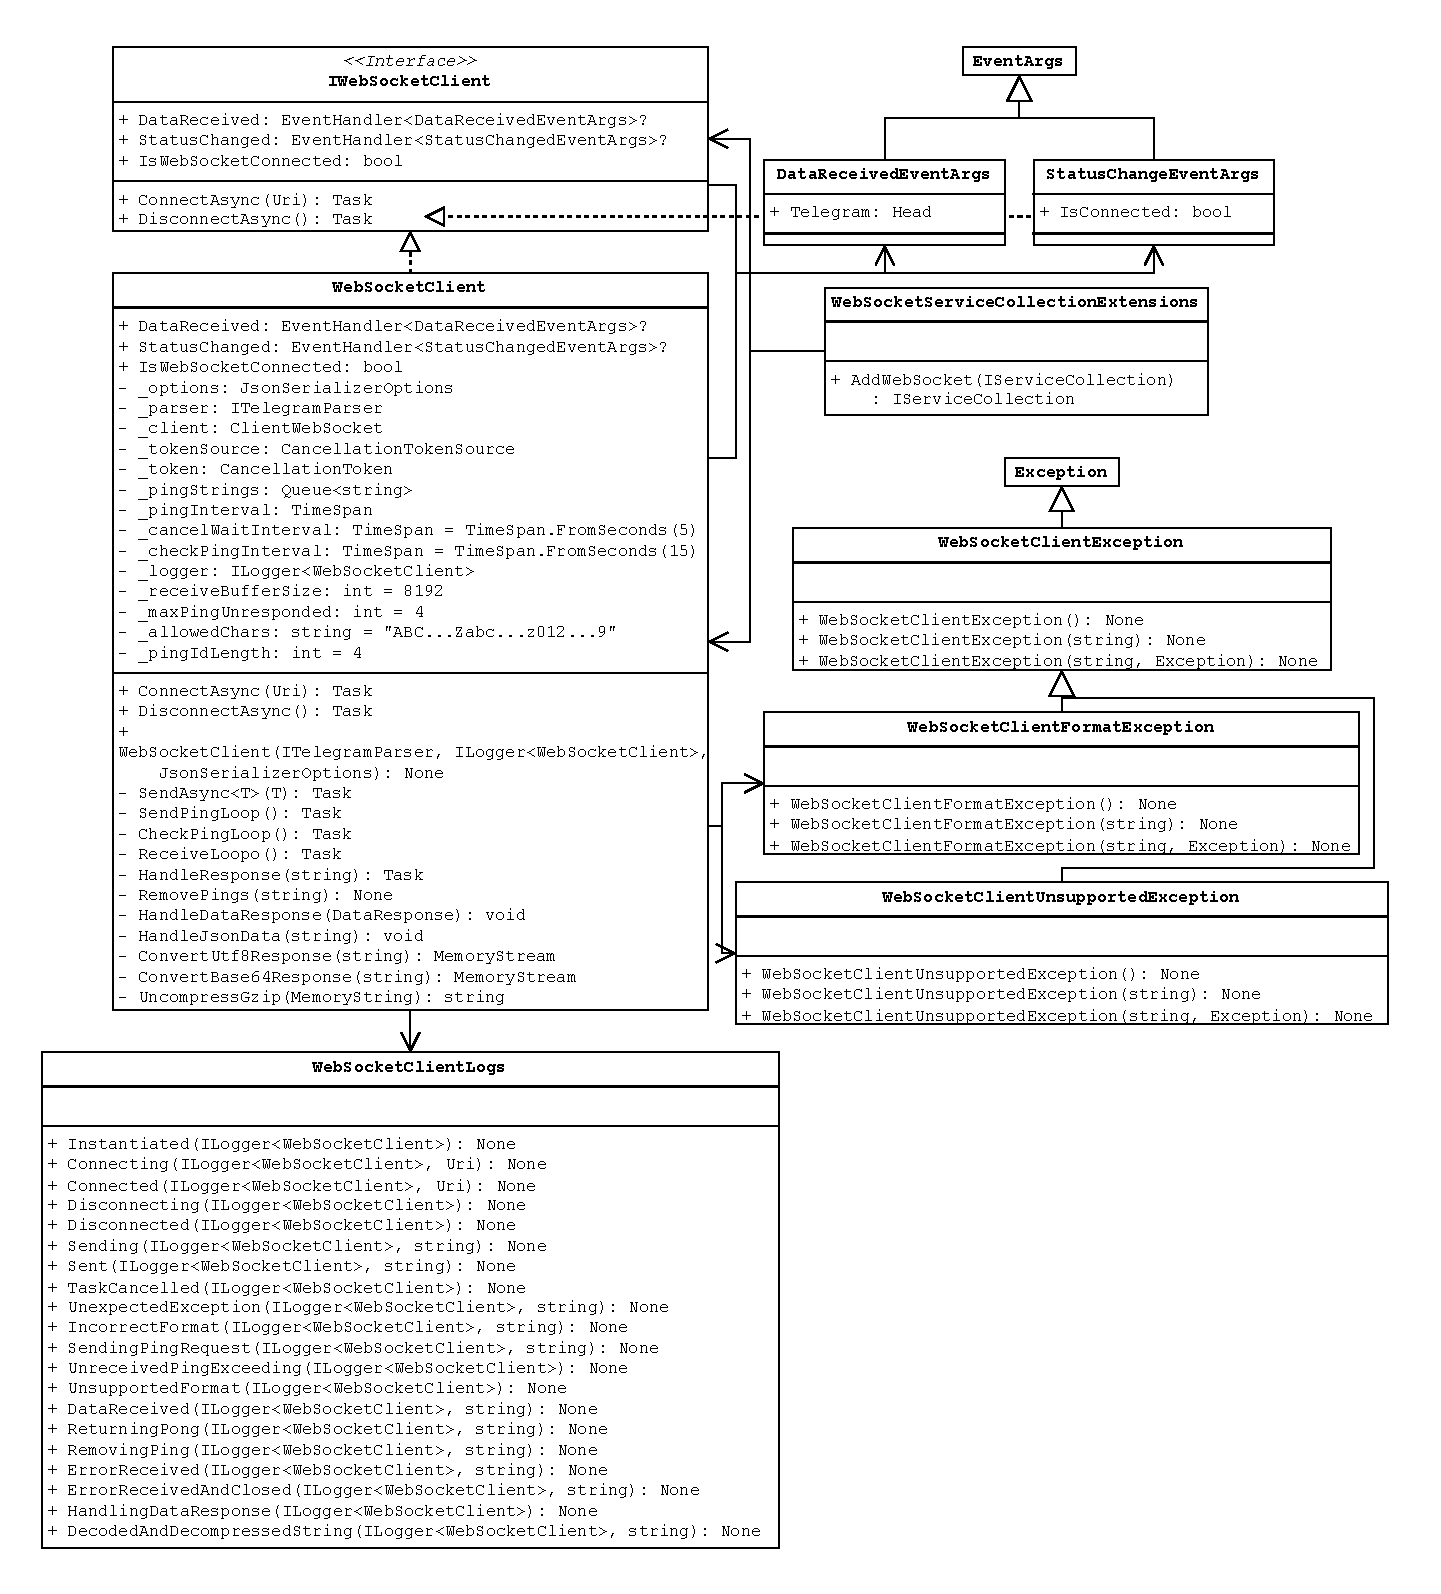
\includegraphics[width=\linewidth]{class-diagram-dmdata-ws.pdf}
    \caption{Class Diagram for DM-D.S.S WebSocket}
    \label{fig:class-diagram-dmdata-ws}
\end{figure}


The modelling of the DTOs for WebSocket is particularly interesting. They are all internal, since they are just designed for internal usage, and not for exposing to external code. First, a \textbf{base record class} \Code{ResponseBase} is implemented, which contains the type of the response in an enumeration, \Code{MessageType}. Contra-intuitively, it is \textbf{not virtual}, since we would like to first parse the data to this, determine the type, and then parse further to get the concrete type of the response depending on the type received. Different concrete types will have different \Code{MessageType}, which is an example of \textbf{polymorphism}.

The five different types of responses, and including the two requests are all inherited from this. The reason is that they all share the same behaviour with the \Code{MessageType}.

The \Code{CompressionType} and \Code{EncodingType} are described as enumerations rather than strings, since they can only take finitely many values, and this allows for easier comparison, and preserves type safety (unlike strings, which might lead to meaningless results).

Apart from this, other compositions of record classes to represents DTOs is just normal behaviour, same as what the API described. Figure \ref{fig:class-diagram-dmdata-ws-dto} gives the class diagram for the DTOs involved. Notice how inheritance and polymorphism is involved.

\begin{figure}[htp]
    \centering
    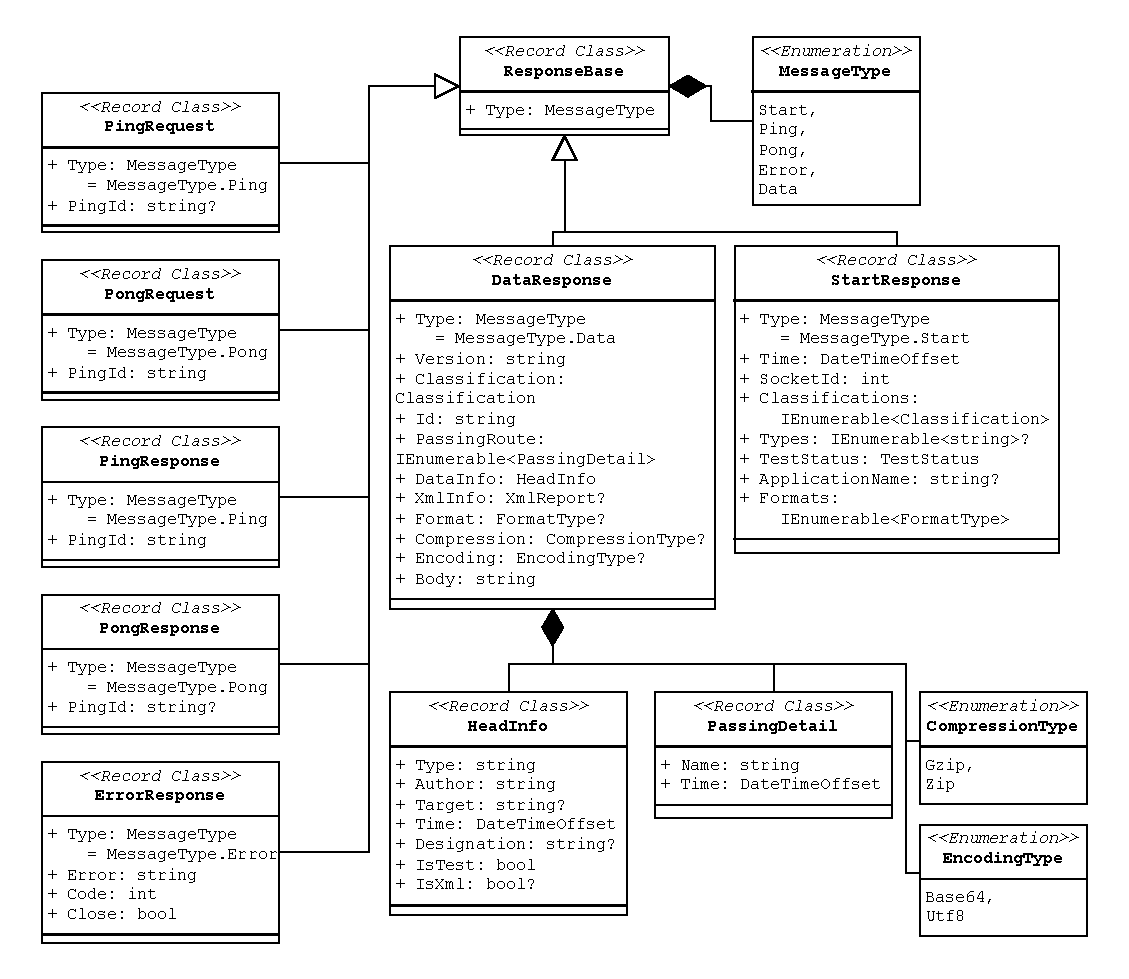
\includegraphics[width=\linewidth]{class-diagram-dmdata-ws-dto.pdf}
    \caption{Class Diagram for DM-D.S.S WebSocket DTOs}
    \label{fig:class-diagram-dmdata-ws-dto}
\end{figure}

This service depends on the common DTOs, and the telegram parser (but not the telegram fetcher, which releases its dependency on the authentication). This means that \Code{ITelegramParser} is \textbf{aggregated} within \Code{IWebSocketClient}, but not \textbf{composed}, just like with \Code{ITelegramRetriever}. In the dependency injection, the \Code{ITelegramParser} will be injected as well, but \textbf{singleton} pattern ensures there is only one of them in play, commonly shared.

\subsection{Design of UI Classes with MVVM Pattern}

\subsubsection{Services}

\paragraph{Logging}

Since the use of the \textbf{adaptor pattern} and \textbf{factory pattern} in logging is described before (for Avalonia and File Logger respectively), a class diagram is included here on how this is in Figure \ref{fig:class-diagram-services-logging}.

\begin{figure}[htp]
    \centering
    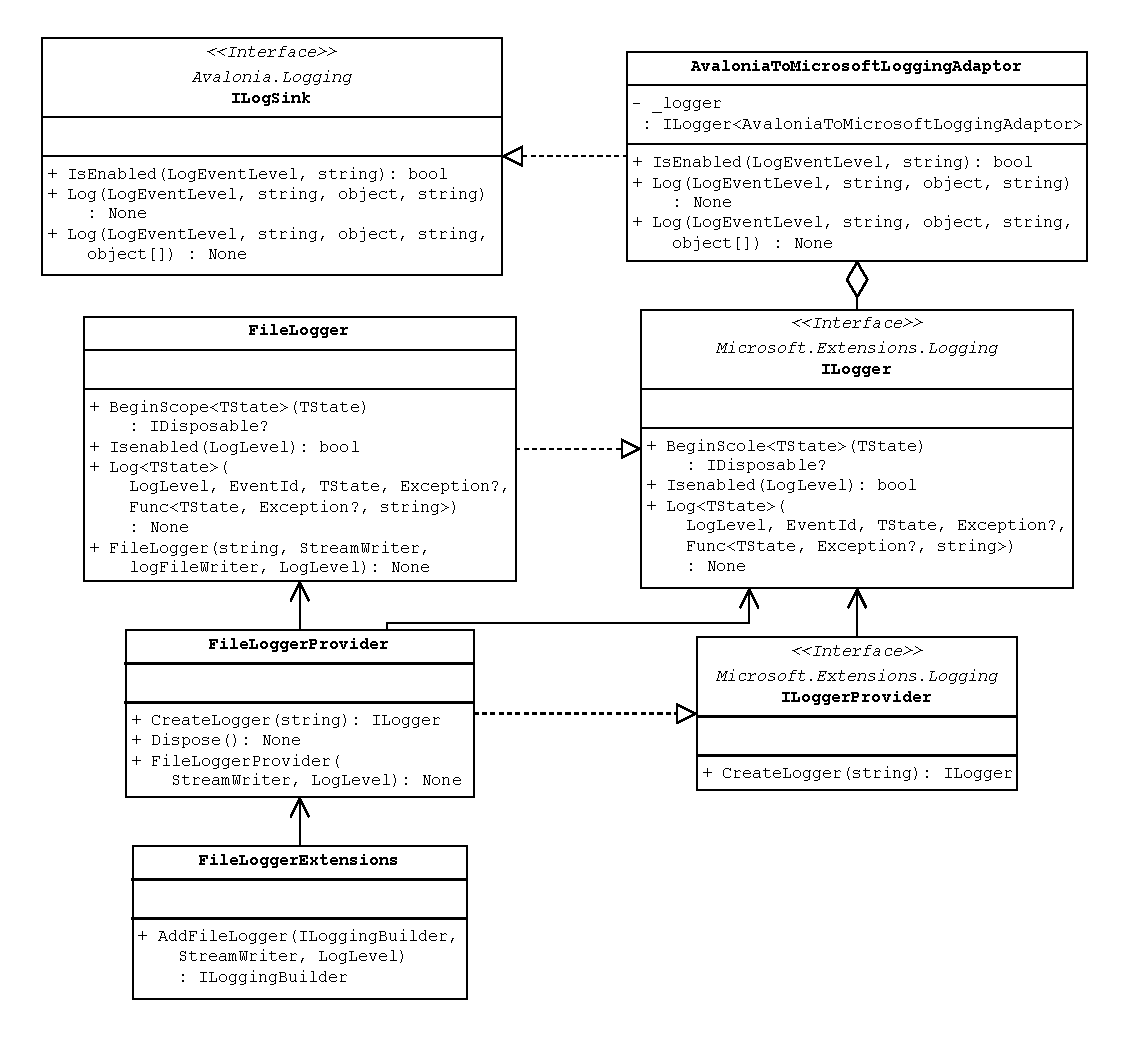
\includegraphics[width=\linewidth]{class-diagram-services-logging.pdf}
    \caption{Class Diagram for Logging Services}
    \label{fig:class-diagram-services-logging}
\end{figure}

\paragraph{Resources}

There are multiple map resources shared across different pages, and they are stored in the \Code{MapResourcesProvider} class, which includes the shape files, the styles for the hypocentres, and the prefectures of Japan (which is further stored in the \Code{PrefectureData} class).  The class diagram for this is in Figure \ref{fig:class-diagram-services-maps}.

\begin{figure}[htp]
    \centering
    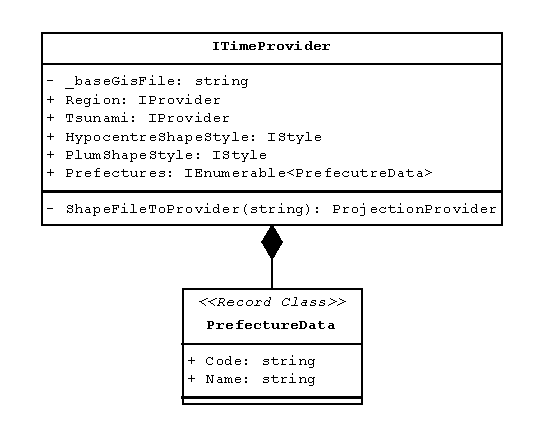
\includegraphics[width=0.5\linewidth]{class-diagram-services-maps.pdf}
    \caption{Class Diagram for Map Resources}
    \label{fig:class-diagram-services-maps}
\end{figure}

\paragraph{Time Abstraction}

Although there is an abstraction for a time provider provided by Microsoft as well, the author preferred to implement his own in the application, since the Microsoft one is too heavy but also lacks some functionality at the same time. It only achieves two things: getting the current time, and convert the time to JST, Japanese Standard Time, for communication with the Kmoni APIs. The class diagram for this is in Figure \ref{fig:class-diagram-services-time}.

\begin{figure}[htp]
    \centering
    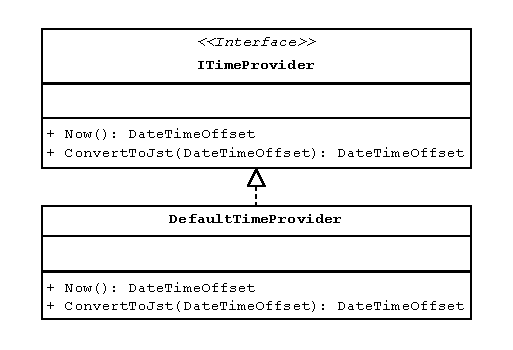
\includegraphics[width=0.5\linewidth]{class-diagram-services-time.pdf}
    \caption{Class Diagram for Time Abstraction}
    \label{fig:class-diagram-services-time}
\end{figure}

This design might look trivial, but this first means that time could be mocked up for unit testing, and secondly past earthquakes are easier to be recreated, since a mock time provider could be provided to mock time in the past, and finally it improves code readability and code reusability, especially with the conversion of time to JST. There could also be a further functionality added, in the future where necessary, for the user to indicate whether they would like time to be displayed locally, or in JST, or in UTC.

\paragraph{Kmoni Settings Manager}

The reason why this (Kmoni) settings in particular is separated from other settings and have a full set of abstractions/options/DTO, is that it has its unique complexities: it is shared between the setting page and the real-time page, it involves the writing of the current option to a file, and it has default options if the file was not able to read/does not exist.

The \textbf{abstraction} involved here is the interface \Code{IKmoniSettingsHelper}, which exposes the current measurement choice, and the current sensor choice. It also has an event to notify when the settings have changed (which is then used to write the new settings to the file, and in the real-time page to update the scale of the GUI to correspond to the new choice). Therefore, in the \textbf{event arguments}, it also includes a copy of the new settings.

There is a \textbf{DTO} called \Code{KmoniSettings}, which stores the sensor type and measurement type, and is serialisable/deserialisable to JSON format, which then could be written to a file/read from a file. Furthermore, this class has \textbf{options} in class \Code{KmoniSettingsHelperOptions}, which contains the file path to store the settings, and the default settings, both to be read from the \Code{appsettings.json} file.

The concrete implementation is \Code{KmoniSettingsHelper}, which is responsible for exposing the property as defined by the interface, while at the same time raising the event if the new sensor choice has changed. It also has logging involved.

Furthermore, there is a \textbf{factory method} provided as extension to the dependency injection container, which reads the current options from the files, and adds the write-to-file method to the event handler. It also does the error handling of the file read and write, and the JSON serialisation/deserialisation -- this shows a clear \textbf{separate of concerns} in the design.

The class diagram for this is in Figure \ref{fig:class-diagram-services-kmoni}.

\begin{figure}[htp]
    \centering
    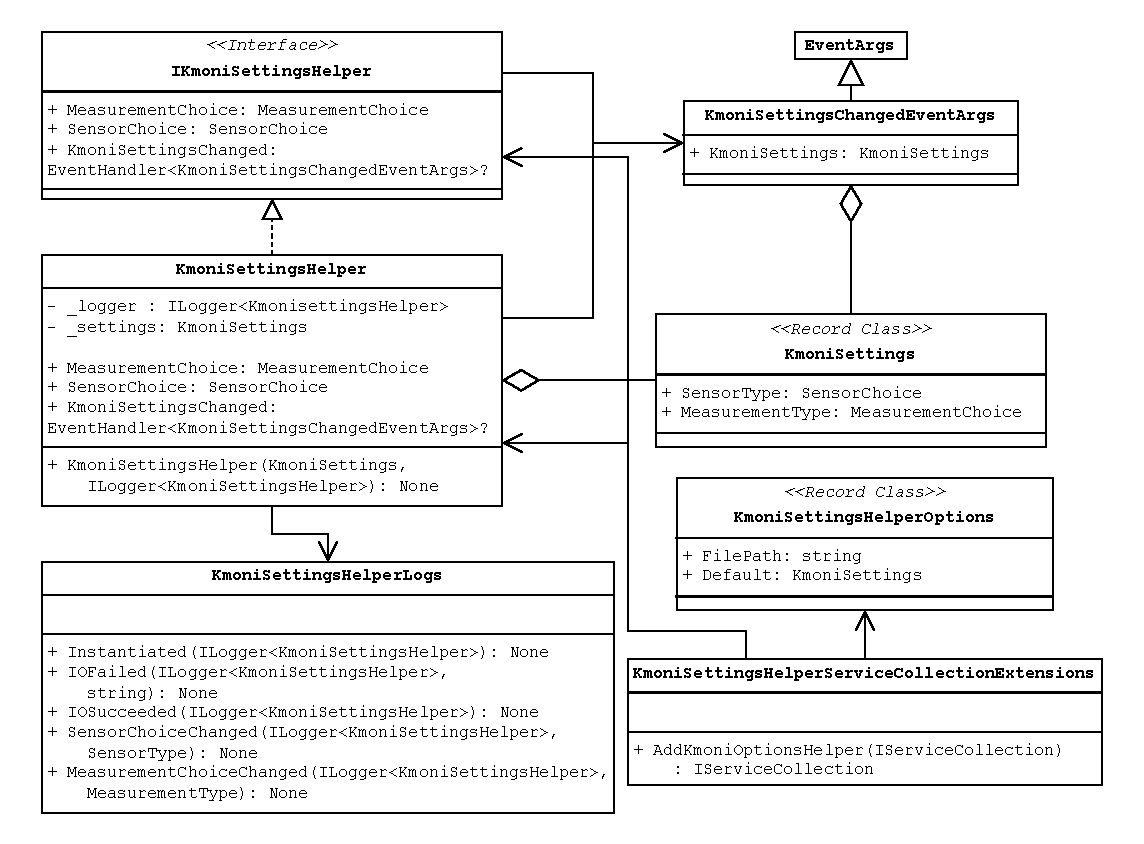
\includegraphics[width=\linewidth]{class-diagram-services-kmoni.pdf}
    \caption{Class Diagram for Kmoni Settings Manager}
    \label{fig:class-diagram-services-kmoni}
\end{figure}

\subsubsection{Views, View Models, and Models}

\paragraph{One-to-one correspondence between view and view model}

This principle is just as straightforward as the title suggests -- there is one view model corresponding to each view, for the view to bind to.

There are four view models involved in the application: the main window (which contains functionality of the sidebar and switching the view-model), the setting page, the past earthquake page, and the real-time page. Figure \ref{fig:class-diagram-ui-view-models} is a class diagram for the design of the view models.

\begin{figure}
    \centering
    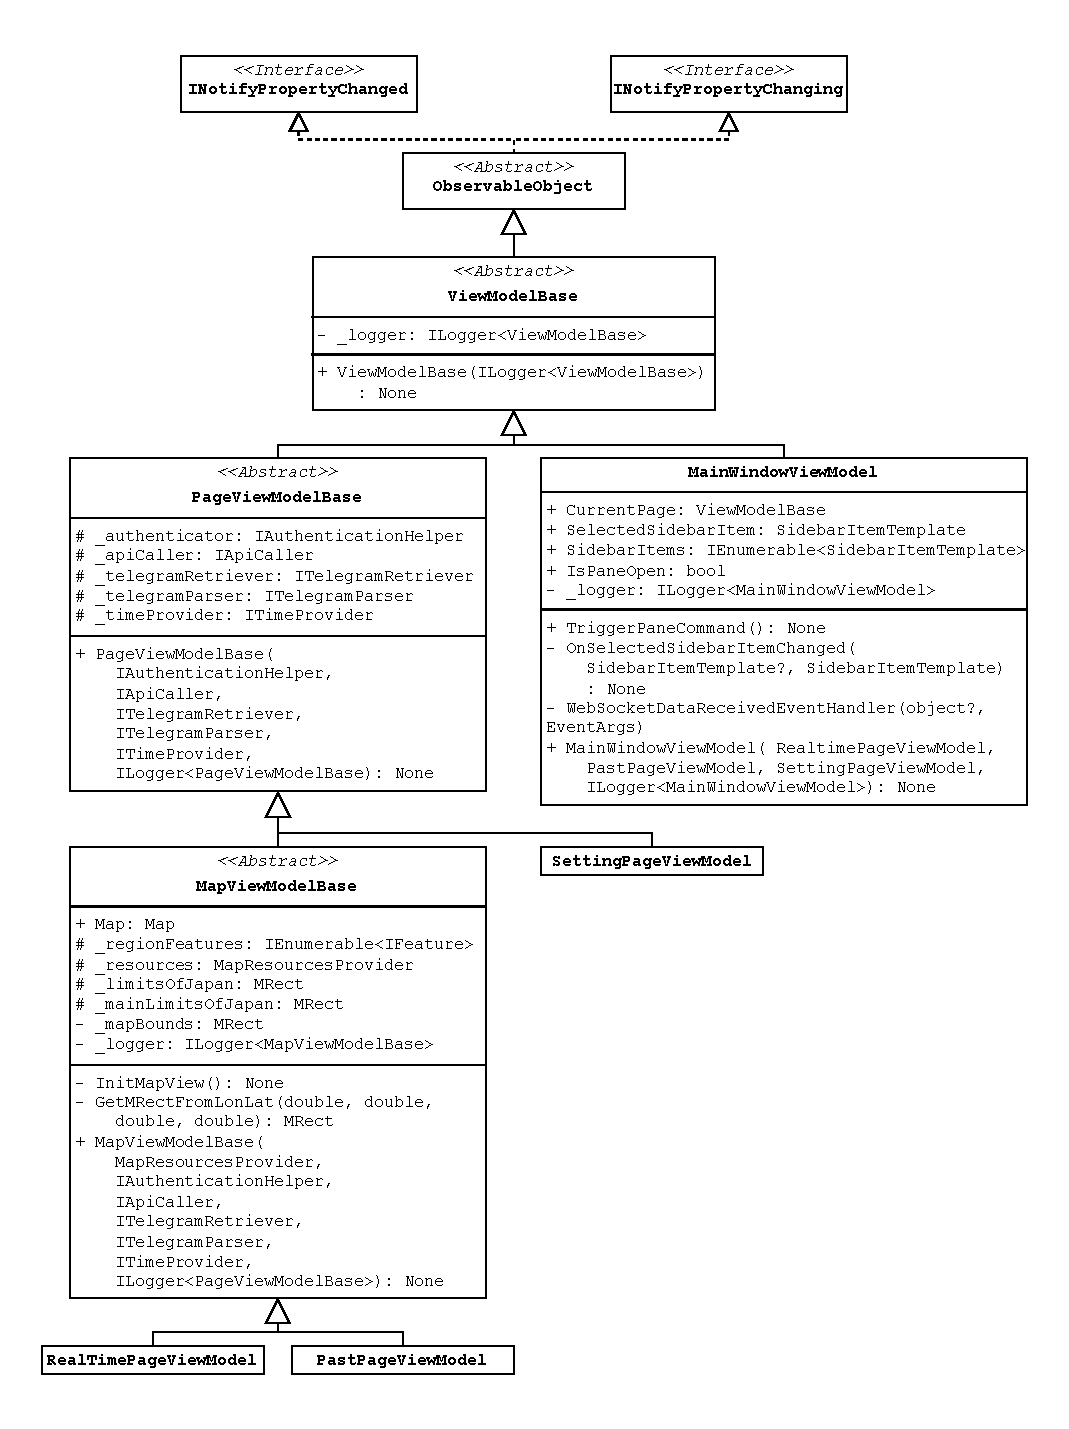
\includegraphics[width=\linewidth]{class-diagram-ui-view-model.pdf}
    \caption{Class Diagram for View Models}
    \label{fig:class-diagram-ui-view-models}
\end{figure}

The details of the view models of the pages will be detailed later.

Even though each view model might look bulky and heavy, the author believes this still does not break the principle of single responsibility -- since each view model is only responsible for one page after all.

\paragraph{Abstract Base Classes}

\textbf{Abstract base classes (ABCs)} are used here which describes the shared parts for view models. All view models inherit from \Code{ViewModelBase}. Then there is a \Code{PageViewModleBase} which is the base view model for view models for a page (i.e. excluding the view model for the window itself). The \Code{MapViewModelBase} inherits from that and provides additional functionalities for the map. \textbf{Protected fields and methods} are used to provide shared functionalities.

\subparagraph{\Code{ViewModelBase}}

This is a class which inherits from the \Code{ObservableObject} from the MVVM toolkit, and only involves the \Code{ILogger} object. This might look unnecessary, but it would be extremely useful in the future, in case we would like to change the MVVM toolkit we use, or if we would like to add more shared functionalities.

\subparagraph{\Code{PageViewModelBase}}

This is a class which inherits from the \Code{ViewModelBase}. It has five protected fields: the authentication helper, the API caller, the telegram retriever, the telegram parser, and the time provider for the application. They are all \textbf{aggregated} but not composed in the classes, since they are not part of the life cycle of the view model, and are passes in as constructors for the view model (as in dependency injection).

\subparagraph{\Code{MapViewModelBase}}

This is a class which inherits from the \Code{PageViewModelBase}. It has a private field marked as an observable property (which makes it public anyway) for the map, and four protected fields for:
\begin{itemize}
    \item the features of the regions read from the shape file;
    \item the static resources for the map, such as the shape files themselves, and the two styles for the hypocentre to be reused;
    \item the limits of Japan; and
    \item the main limits of Japan (containing the tiny islands as well).
\end{itemize}

\paragraph{The Window}

The view model for the main window has quite simple purposes: providing the sidebar to switch between views (view models), and provide a button to expand/retract the side pane as well.

The property \Code{IsPaneOpen} is a boolean indicating whether the sidebar pane is open, and it is bound to the property of the pane. The button to expand/retract side pane is bound to \Code{TriggerPaneCommand}, which changes the boolean value (by XOR with true).

The only model associated with this, is the item displayed in the sidebar, \Code{SidebarItemTemplate}. It is initiated with the instance of the view model, the icon key to display on the sidebar, and the text to display on the sidebar. The view will be able to bound the related properties by accessing the list of sidebar items. Since this instance is created in the constructor of the view model, it is considered as \textbf{aggregation}, since their life cycle is strongly correlated.

Upon the chosen item changing in the sidebar, the \Code{CurrentPage} will change as well, allowing the view of the window to change the binding.

It will also handle the event raised by the real time view model requesting to change the view model to the real time view model, and this will be done within the constructor.

Figure \ref{fig:class-diagram-ui-window} is the class diagram for the window view model and the related components.

\begin{figure}[htp]
    \centering
    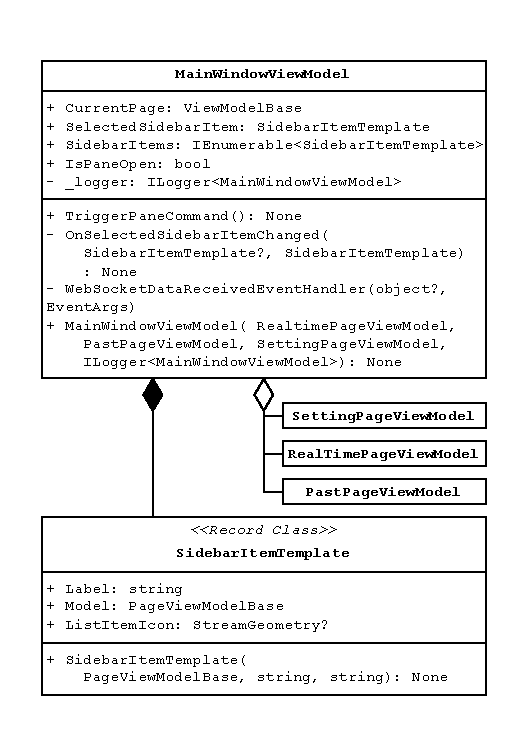
\includegraphics[width=0.5\linewidth]{class-diagram-ui-view-model-window.pdf}
    \caption{Class Diagram for Window}
    \label{fig:class-diagram-ui-window}
\end{figure}

\paragraph{Models for Setting Page}

There are \textbf{four} primary functionalities of the settings page: changing the language setting, the Kmoni setting, the WebSocket settings, and the authentication settings.

Figure \ref{fig:class-diagram-ui-settings} is the class diagram for the settings view model and related components.

\begin{figure}[htp]
    \centering
    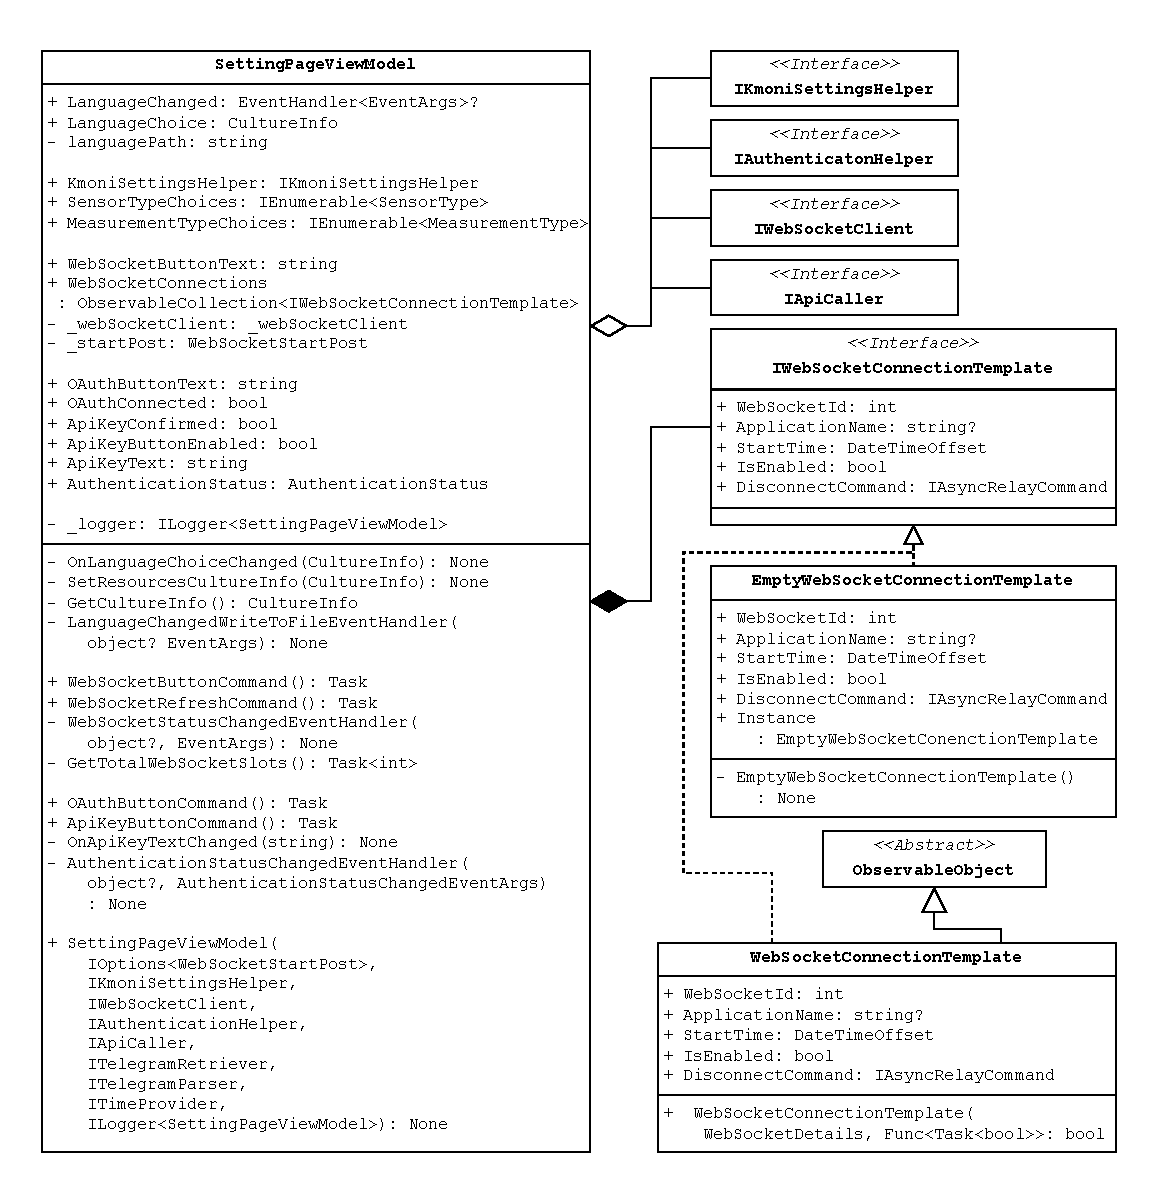
\includegraphics[width=\linewidth]{class-diagram-ui-view-model-settings.pdf}
    \caption{Class Diagram for Settings}
    \label{fig:class-diagram-ui-settings}
\end{figure}

\subparagraph{Language Settings}

There is an \textbf{event}, \Code{LanguageChanged} to be invoked when the language is changed. This is not used in particular for external code -- this is used as a means to clean up what is to be done when the language has changed. In the current design, only two tasks are to be preformed: change the current language of the resources files, and to write it to the file which stores the language. The existence of this event allows the functionality to be extended, such as popping a window for the user to confirm, in the future.

The property \Code{LanguageChoice} is exposed to the view model to bind to the current language choice, and \Code{LanguageChoices} is the list of languages available. To be consistent with the resources file, the type \Code{CultureInfo} is used to represent the language.

\subparagraph{Kmoni Settings}

For the Kmoni settings, there is a \Code{IKmoniSettingsHelper} \textbf{aggregated} within the class, and two lists which contains the choice of the sensor type and the measurement type. The properties in the settings helper are directly bound to the view model, and all properties changed are handled within the settings helper.

\subparagraph{WebSocket Settings}

This part aggregates a \Code{IWebSocketClient}, which is the actual WebSocket connection. There is an event handler for the WebSocket connection status changing, since the view model has to notify the view that certain properties has changed (the current WebSocket status). There is a text to bind to the WebSocket connect/disconnect button (which will change when the WebSocket status is changed), and there is a command bound to it as well to connect/disconnect.

In the table there is a list of current \Code{WebSocketConnections}, which is a \Code{ObservableCollection} of the interface \Code{IWebSocketConnectionTemplate}. The use of the observable collection is since it will be able to notify the view whenever its members has changed. The interface of the WebSocket Connection declares four properties: the WebSocket ID, the application name, the starting time of the connection, and whether the disconnect button is enabled. A method for disconnecting is also provided. This is an example of the \textbf{adaptor} pattern, since it adapts the objects returned by an API call to the contract we have with the view for binding.

The reason why there is a use of the interface here, is because of \textbf{polymorphism}: there are two concrete implementations of this, the first an empty WebSocket connection, which just stays put (and shares a common instance), and the other an actual WebSocket connection, as will be shown in the class diagram below. They behave differently (especially their disconnection command). The actual WebSocket connection also inherit from Observable Object to allow the notification to the view that its properties has changed.

To implement the refreshing the list of current WebSocket connections, there is a separate method to get the number of total WebSockets available to the user (which looks through the user's contracts), and a separate method to list all currently active WebSockets. The observable collection then could be altered to reflect the latest result.

\subparagraph{Authentication Settings}

For the setting for authentication, there is first property exposing the current \Code{AuthenticationStatus} to the view via the authenticator, to display the current authenticator. There is also an event handler to handle the authentication status changed event, which notifies the properties that are related with the current authentication status.

There are two commands exposing to the view model, the button to set the current API Key, and the button to connect/disconnect from OAuth 2.0. There is also a string for the current API Key Text, a string for the text to display on the OAuth button, a boolean for whether OAuth connection is connected, a boolean for whether API Key is confirmed, and button for whether the API Key button is enabled (i.e. the API Key fits the format, which will be checked every time if the API Key is currently valid).

\paragraph{Past Earthquake Page}

Splitting up the functionality for the past earthquake page, there are two main functionalities: the past earthquake list, and the past earthquake details display. Hidden behind this is a functionality to retrieve and cache the list of earthquake observation stations (which we will regard as the third functionality).

Figure \ref{fig:class-diagram-ui-past} is the class diagram for the past earthquake view model and related components.

\begin{figure}[htp]
    \centering
    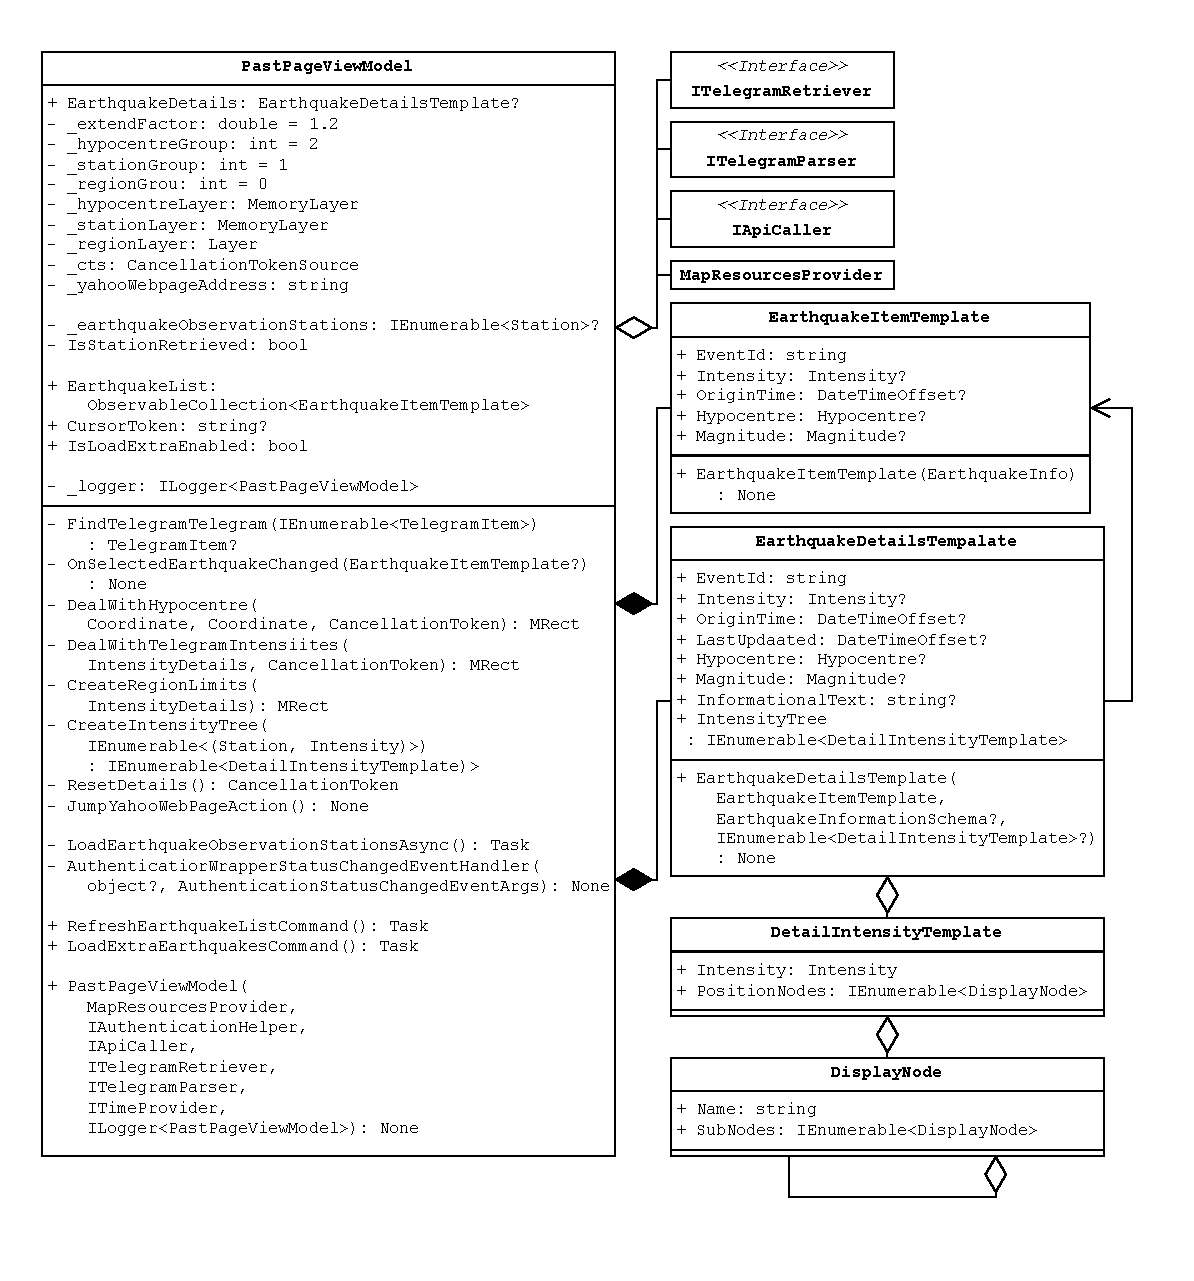
\includegraphics[width=\linewidth]{class-diagram-ui-view-model-past.pdf}
    \caption{Class Diagram for Past Earthquake}
    \label{fig:class-diagram-ui-past}
\end{figure}

\subparagraph{Earthquake List}

To achieve the list of earthquakes, the user would have to press the refresh button, which calls the command associated with it, and attempts to fetch a list of earthquakes, stored into an observable collection. \textbf{Note that the observable collection is annotated with observable property as well}, since we could just totally re-set the list to a new one, and the view will be able to reflect the change. In this method, the cursor token will also be stored to a private field, and used to load extra earthquakes. There is a boolean field reflecting whether the load extra button is enabled, by checking if the cursor token is null.

The model to store the earthquake list item takes one earthquake from the API call as in the constructor, and changing it to the contract to the view, which is another demonstration of the \textbf{adaptor pattern}. It only keeps the necessary properties for binding as well.

\subparagraph{Observation Stations}

To load the list of earthquake observation stations, the user has to be authenticated first. If the constructor detects that the authenticator is in an authenticated stage, the constructor will attempt to fetch the station list at the start. When the authentication status is changed, there is also an event handler that attempts to fetch the list as well.

There is a method to load the stations manually as well, and allows for methods to check for if the list is initialised, before attempting to use it.

\subparagraph{Earthquake Details}

This section has the most details and has the most complicated functionalities. First, three layers are repeatedly used over the life cycle of the application: the layer for the hypocentre, for the observation stations, and for the regional intensities. When a new earthquake is selected, it will not attempt to create a new layer -- instead, it will change the data/style of a layer, and notify the layer that the data has changed.

Secondly there are constants defining the layer of the groups. It is designed such that the hypocentre always stays at the top of the map, stations the next, and the hypocentre in the bottom layer. There is also a \textbf{cancellation token source} -- this is involved, since if the user has changed the mind of which earthquake they want to view the details of, before the details has been reflected on the map, we do not want it to be reflected any more -- and we would like to cancel the asynchronous task. Therefore, in the rest details method, it will cancel and dispose of the current cancellation token source, and set up a new one for the next chosen earthquake.

There is a method to jump to the Yahoo earthquake page for the details of the earthquake as well, using a constant private field of string for the URL to be formatted.

Now comes the interesting part on how to deal with when a new earthquake item is selected.

\begin{itemize}
    \item MVVM invokes the \Code{OnSelectedEarthquakeChanged} method, which first resets the current earthquake details, and then attains a new cancellation token for the current earthquake.
    \item The method gets a list of telegrams for the current earthquake, and uses \textbf{filter, group by, select and order} methods as in \Code{FindEarthquakeTelegram} to decide the most suitable telegram to get the information from, as described earlier in the design for the UI page.
    \item It creates the \textbf{intensity tree} and the \textbf{regional limits} (map bounds of regions which observed intensity) for the earthquake by calling the \Code{DealWithTelegramIntensities} method.
    \item It marks the hypocentre on map and obtains limits for the hypocentre by \Code{DealWithHypocentre} method.
    \item It zooms the map to the union of the regional limits and hypocentre, multiplied by a constant \Code{_extendFactor}.
    \item It creates the details of the earthquake to display on the side panel, using the intensity tree created, the acquired telegram, and the earthquake list item.
\end{itemize}

In the \Code{DealWithHypocentre} method, it will change the features of the hypocentre layer and notify the feature has changed, and return the limits for the hypocentre.

In the \Code{DealWithTelegramIntensities} method, it will first \textbf{filter} where the intensity is not unknown, and \textbf{join} it with the list of observation stations.

Then, it will call method \Code{CreateRegionLimits} which \textbf{aggregates} the region limits of each region involved using the union operation, and the \Code{CreateIntensityTree} method which \textbf{joins} the station data further with a list of prefectures, and group by intensities, and group by prefecture, region, and finally by city, to create a \textbf{tree} structure.

There is a significant use of \textbf{list-manipulation methods} here, using existing \textbf{LINQ} methods including join, aggregate, select, where, group by, order by, and first.

As for the models used, \Code{EarthquakeDetailsTemplate} is just \Code{EarthquakeItemTemplate} with some more properties to display on the sidebar, and takes it and the telegram and the intensity tree within the constructor.

The particular interesting thing here is the \textbf{intensity tree}: it is a tree \textbf{with different data types} on different depths. Its root could be considered as the earthquake detail object, and on its first layer, the \textbf{intensity} is stored, but afterwards it stores a location, which could simply be it stores a \textbf{string}.

Therefore, there are two classes involved here: \Code{DetailIntensityTemplate}, which is for the first layer, having an intensity and a list of \Code{DisplayNode} (which is its children), which has a name, and a list of \Code{DisplayNode} (which is its children). The whole tree is stored in a list of detail intensity template, which is a tree itself. Therefore, as shown in the class diagram, display node is aggregated within itself and detail intensity template, which is further aggregated into earthquake details template (it is not composition since it is provided at the constructor of earthquake details template).

\paragraph{Real-Time Page}

This is the view model with the most functionalities, but we can split it up into five parts: common parts of the view model, handling EEW, handling Tsunami, handling WebSocket, and Kmoni monitor functionality. Figure \ref{fig:class-diagram-ui-real-time} is the overall class diagram for the real-time view model and related components.

\begin{figure}[htp]
    \centering
    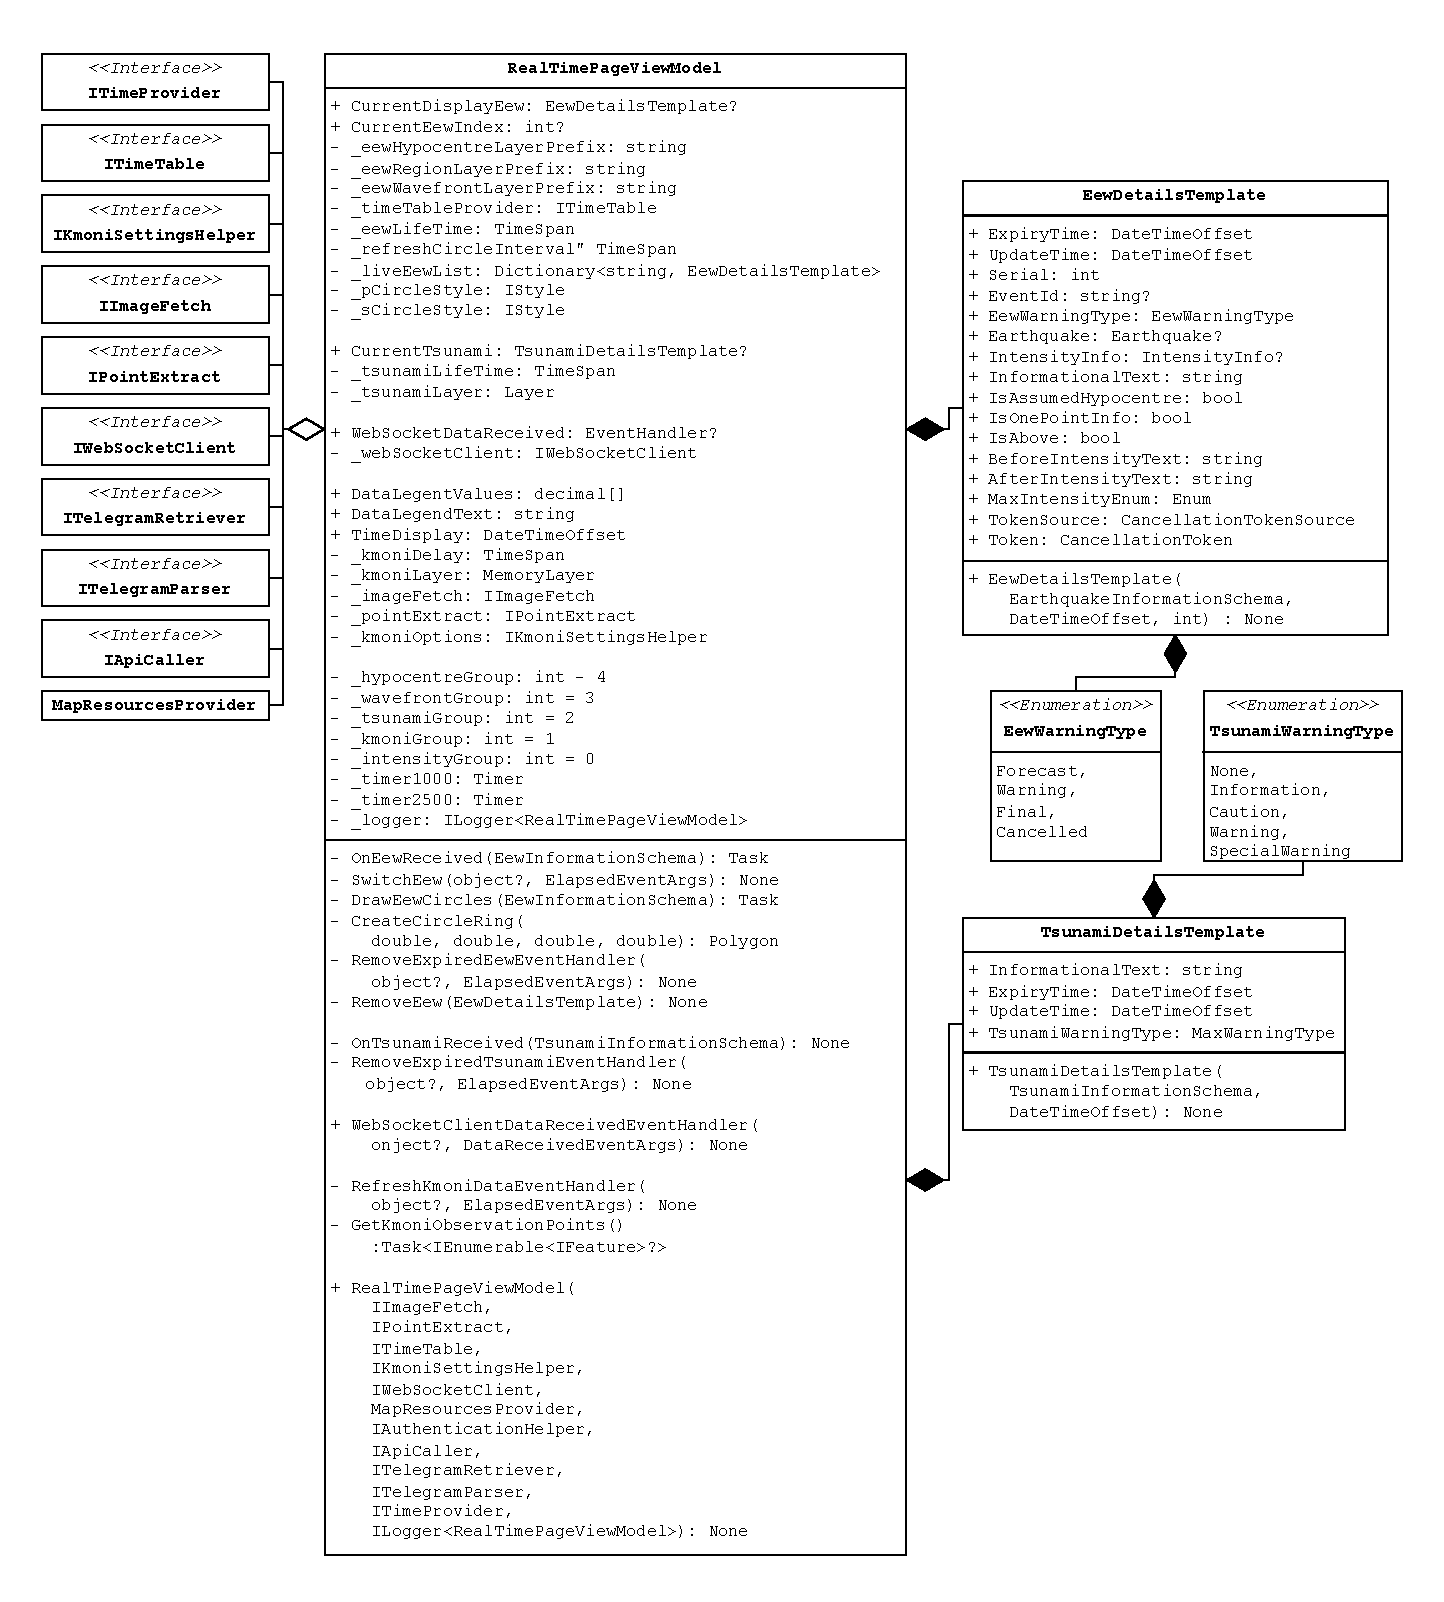
\includegraphics[width=\linewidth]{class-diagram-ui-view-model-real-time.pdf}
    \caption{Class Diagram for Real-Time Page}
    \label{fig:class-diagram-ui-real-time}
\end{figure}

\subparagraph{Common Parts}

There are two \textbf{timers} shared by all the parts: a timer that invokes events every second (which includes refreshing the time display, removing expired EEW/Tsunami warnings, and refreshing the Kmoni layer), and a second one that invokes events every 2.5 seconds (which includes the switching of the EEW, if applicable). These event subscribers will be added to the timer within the constructor.

Furthermore, the management of group layers from to bottom is as follows, the layer number defined as a constant integer field (for code reusability and readability):
\begin{itemize}
    \item Hypocentre,
    \item Wavefront,
    \item Tsunami,
    \item Kmoni,
    \item Intensity Regions.
\end{itemize}

\subparagraph{EEW}

The key part of the EEW is that there could be multiple EEW in effect at the same time. However, there is one thing that is unique for each EEW: their event ID. Therefore, a suitable data structure to store this collection of EEWs is a \textbf{dictionary}, with the event ID in \textbf{string} as the key, and the EEW in \Code{EewDetailsTemplate} as the value.

This naturally leads to switching the current display EEW. This is controlled by \Code{CurrentEewIndex}, a nullable integer for the current EEW index, and \Code{CurrentDisplayEew}, a nullable \Code{EewDetailsTemplate} which has a get method using the index to display the earthquake. When the \Code{SwitchEew} event handler is invoked, it will do the follows:
\begin{itemize}
    \item If the number of current EEWs is zero, set the index to null;
    \item Else, if the current index is null, set the index to zero;
    \item Else, increment the current index by one, and modulo the length of the number of current EEWs.
\end{itemize}

The design of the \Code{EewDetailsTemplate} is as follows: apart from the standard information to display, there are two properties of type string, \Code{Before} and \Code{AfterIntensityText}, which gives the text to display before/after the intensity (e.g. if the intensity provided in the EEW is 'above 6+', then the before text will be 'above'. In Japanese the after text will be '以上', since the sequence in the language is different.) There is also an enumeration determining which enumeration to display (if it is (6-, 6+), then it will display 6+; but if it is above 6- i.e. (6-, above), then it will display 6-). Finally, notice there is a cancellation token source and cancellation token here -- this indicates whether this EEW has already been removed from the collection of EEWs, to allow for asynchronous operation to halt.

The type of the EEW is described by the enumeration \Code{EewWarningType}, and the logic of deciding the type of the EEW was discussed before in the design of the UI.

The handler for receiving an EEW is \Code{OnEewReceived}. First, it determines if the EEW is newer than the current EEW in the collection, with the same event ID (making the decision based on the serial number). If not, then it will do nothing; if yes, then it will remove the EEW in display. Then, it will plot the coordinates of the hypocentre on the map, using the corresponding shape style depending on whether the hypocentre is assumed, and also display the regional intensities colouring on the maps.  Finally, it will start a long-running background task on a separate thread to draw the wavefronts for the EEW.

This is the asynchronous \Code{DrawEewCircles}. First it checks if the EEW fits the condition to draw the wavefronts (e.g. is the earthquake, hypocentre, origin null, or is it an assumed hypocentre). If not, it will then check if the depth is within the acceptable range. If all the checks passed, it will then insert two layers onto the map, one for the P-Wave and another for the S-Wave, which will be re-used throughout the duration of the EEW, updating only the features.

Then there is a while loop, which will continue until the cancellation is requested. During the loop, it will find the time that the earthquake has elapsed, and find the distance the seismic waves has travelled through by checking with \Code{ITimeTable}, and adding the feature onto the layer, and notifying the layer that its data has changed. The loop will sleep for a certain amount of time, and then repeat the process. After quitting the loop, the layers will be removed from the map.

\Code{CreateCircleRing} is a method designed to draw a circle in \Code{Polygon} at the given position and radius, to a good quality. Basic geometry is used here, but since the projection of the map changes the length, a magic constant is introduced to the radius to correctly plot the circle with approximately the correct radius.

The method to remove an EEW is as follows (assuming the EEW is removed from the collection): the cancellation token source will be cancelled and disposed of, and then the maps layer of hypocentre and regions, with the correct event ID attached to, will be removed. This will also be regularly called by a method which is invoked by the timer to regularly iterate through the dictionary to see if there are any expired EEWs.

\subparagraph{Tsunami}

Since it is almost certain that there is only one tsunami warning in effect at one time, the model \Code{CurrentTsunami} is simply a single object of type \Code{TsunamiDetailsTemplate?}. The tsunami layer is also initialised once and used throughout the lifetime of the application, since the data source (shape file) stays the same, and only the colouring of the shape file (the style) changes.

The first method involved here is \Code{OnTsunamiReceived}, which handles the tsunami when it is received. It is in charge of finding the valid date time of the tsunami (which is as indicated on the telegram, or if not then \Code{_tsunamiLifeTime} which is 2 days in the program), and setting the \Code{CurrentTsunami} object and changing the style of the map.

The second method involved is \Code{RemoveExpiredTsunamiEventHandler} which is subscribed to the one-second timer. It checks if the current tsunami has expiry time before the current time (as indicated by the time provider), and if so, set the current tsunami to null and set the layer style to null as well.

In terms of the models involved, \Code{TsunamiDetailsTemplate} is a record class that holds the details of the tsunami, including its informational text, expiry time, update time, and maximum tsunami warning type of the tsunami warnings of shorelines issued (using the \textbf{max} method in \textbf{LINQ}, which is an \textbf{aggregate}). The tsunami warning type is an enumeration, containing the tsunami warning type level. JMA uses a code to describe the tsunami warning type, so a conversion method is provided as well.

\subparagraph{WebSocket}

This part consists of two functionalities: handling the WebSocket data received event (passing it to the appropriate handler for EEW or for Tsunami), and a separate event indicating data received from WebSocket (requesting main window to switch view model to the real-time page) named \Code{WebSocketDataReceived}. The former is achieved by subscribing to the event in the WebSocket client (which is done in the constructor), and the latter will be raised in the event handler. Notice that subscription to the event raised by this will be done in the window view model.

\subparagraph{Kmoni Monitor}

The first functionality this part achieves is displaying the \textbf{legend} for the colours of the Kmoni layer. This consists of two parts: the text for the legend in string \Code{DataLegendtext}, displaying the type and units of the data measured, and the values on the scales of the legend in a decimal array \Code{DataLegentValues}. The latter involves \textbf{list manipulation} using \textbf{LINQ method select} to \textbf{map} normalised height to the scale of the data that is concerned.

The second functionality is to display the Kmoni data on the map. To improve performance, the same layer \Code{_kmoniLayer} is used, and only the data within the layer will be updated to be reflected on the map. To prevent 404 requests, a time delay is in \Code{_kmoniDelay} which is subtracted from the current time when request is sent to fetch the image and extract the points. This is done by \Code{RefreshKmoniDataEventHandler}, which fetches the Kmoni data, and updates the layer if the fetch is successful. The \Code{GetKmoniObservationPoints} is the method called which actually fetches the data and converts them to the feature to display on the map.

\subsection{Design of DTOs (Record Classes)}

\subsubsection{Common (Reusable) DTOs}

In principle, the DTOs should be contained in the namespace for the abstraction requiring the use of the DTO, such as the API calls, the telegrams, or the WebSockets, and exposed to the user where necessary. However, there are some DTOs to be reused, primarily because they are shared across the different parts of the DM-D.S.S. API, WebSocket and telegram services.

\paragraph{JSON Components}

DM-D.S.S. designed \textbf{JSON components} for the application \autocite{dmdata-references-json}, which improves the reusability of typed records over the application. These components include:
\begin{itemize}
    \item The description of the earthquake; which further incorporates:
          \begin{itemize}
              \item The hypocentre (including the depth and the coordinate);
              \item The magnitude;
          \end{itemize}
    \item The coordinate position of some property.
\end{itemize}

This makes the records highly reusable, and these will be reused for the API calls (since it is included in the earthquake list and event calls), and the telegrams as well.

\textbf{Enumerations are used wherever possible.} In this case, it means that strings which can only take finitely-many enumerable values will be modelled as an enumeration. In this component, it means that:
\begin{itemize}
    \item The condition for the depth (very shallow 'ごく浅い', very deep '700km以上',  unclear '不明') are modelled with \Code{DepthCondition};
    \item The condition for the magnitude (unknown 'M不明', very big 'M8を超える巨大地震') are modelled with \Code{MagnitudeCondition};
    \item The unit for the magnitude (JMA magnitude 'Mj', normal magnitude 'M') are modelled with \Code{MagnitudeUnit};
    \item The source for the information of the earthquake (the earthquake advisory centres available) are modelled with \Code{Source};
    \item The geodetic coordinate used (world geodetic coordinate '世界測地系', Japanese geodetic coordinate '日本測地系') are modelled with \Code{Geodetic}.
\end{itemize}

\paragraph{Telegrams}

Several components of the telegram are shared between different parts of the DM-D.S.S. functionality. Those include:
\begin{itemize}
    \item \Code{XmlReport} which composes of \Code{XmlHead}, \Code{XmlControl}, and describes the key components of the XML telegram. This is used within the API call for the earthquake event, and the data response from the WebSocket.
    \item \Code{SchemaVersionInformation}, which includes the type and the version for the JSON schema used. It is shared with the API component (because in each telegram retrieved for earthquake event the schema will be included), and for parsing the telegram.
    \item \Code{TelegramStatus} and \Code{TelegramType}, which describes the status and the type of the telegram. They are composed within \Code{XmlHead}, and for \Code{Head} in the telegram component as well (described later).
\end{itemize}

Note that \Code{TelegramStatus} and \Code{TelegramType} are modelled as enumerations, since they only take a finite number of values, although provided by string from the original API.

\paragraph{Enumerations}

There are also a couple of other shared enumerations within the DM-D.S.S. services. They are all modelled from strings which can only take finitely many values.
\begin{itemize}
    \item \Code{Classification}, which could be used to describe the classification for a contract that user subscribed to, or the classification of a telegram.
    \item \Code{Intensity} for earthquake intensity, \Code{LgCategory} for LPGM motion category, and \Code{LgIntensity} for LPGM intensity;
    \item \Code{FormatType} and \Code{TestStatus} for describing the format of a particular telegram (JSON, XML, Alpha Numeric or Binary) and the test status (whether it is a test or not), both used for setting up the WebSocket and in the WebSocket service.
\end{itemize}

\subsubsection{API Calls}

Since all API Calls must share the response ID, response time, and response status properties, this could be modelled as an \textbf{abstract base class} (record class) for the API calls. This is the \Code{ApiBase} class, on the top of the diagram, composing of an enumeration for the status of the class.

Inheriting from it are two types of responses: a \textbf{successful} response (which is abstract as well), and an \textbf{error} response (which is concrete). The error response composes the details of the error within as a DTO.

There are three responses further abstracted, each inheriting from the previous one:
\begin{itemize}
    \item a \textbf{list} response, which contains a \Code{ItemList} containing all the items in the \Code{item} property in the serialised JSON;
    \item a \textbf{token} response, which contains a \Code{NextToken} property for the next API call; and
    \item a \textbf{pooling} response, which contains the next pooling and next pooling interval properties for the next API call.
\end{itemize}

As described in the previous behaviour of the API responses:
\begin{itemize}
    \item \Code{WebSocketStart} and \Code{GdEarthquakeEvent} response are success responses and compose f only the details of the response;
    \item \Code{ContractList} and \Code{EarthquakeParameter} contains a list of contracts/stations within the response. In the parameter response, in addition to this, it also contains the last changed time for the data, and the version information;
    \item \Code{WebSocketList} contains a token but not a pooling token, and contains a list of WebSocket details; and finally
    \item \Code{GdEarthquakeList} contains a list of past earthquake information, and is a pooling response.
\end{itemize}

This design is accurately reflected in Figure \ref{fig:class-diagram-dmdata-api-dto} which shows a clear use of \textbf{inheritance, composition and abstract classes}.

\begin{figure}[htp]
    \centering
    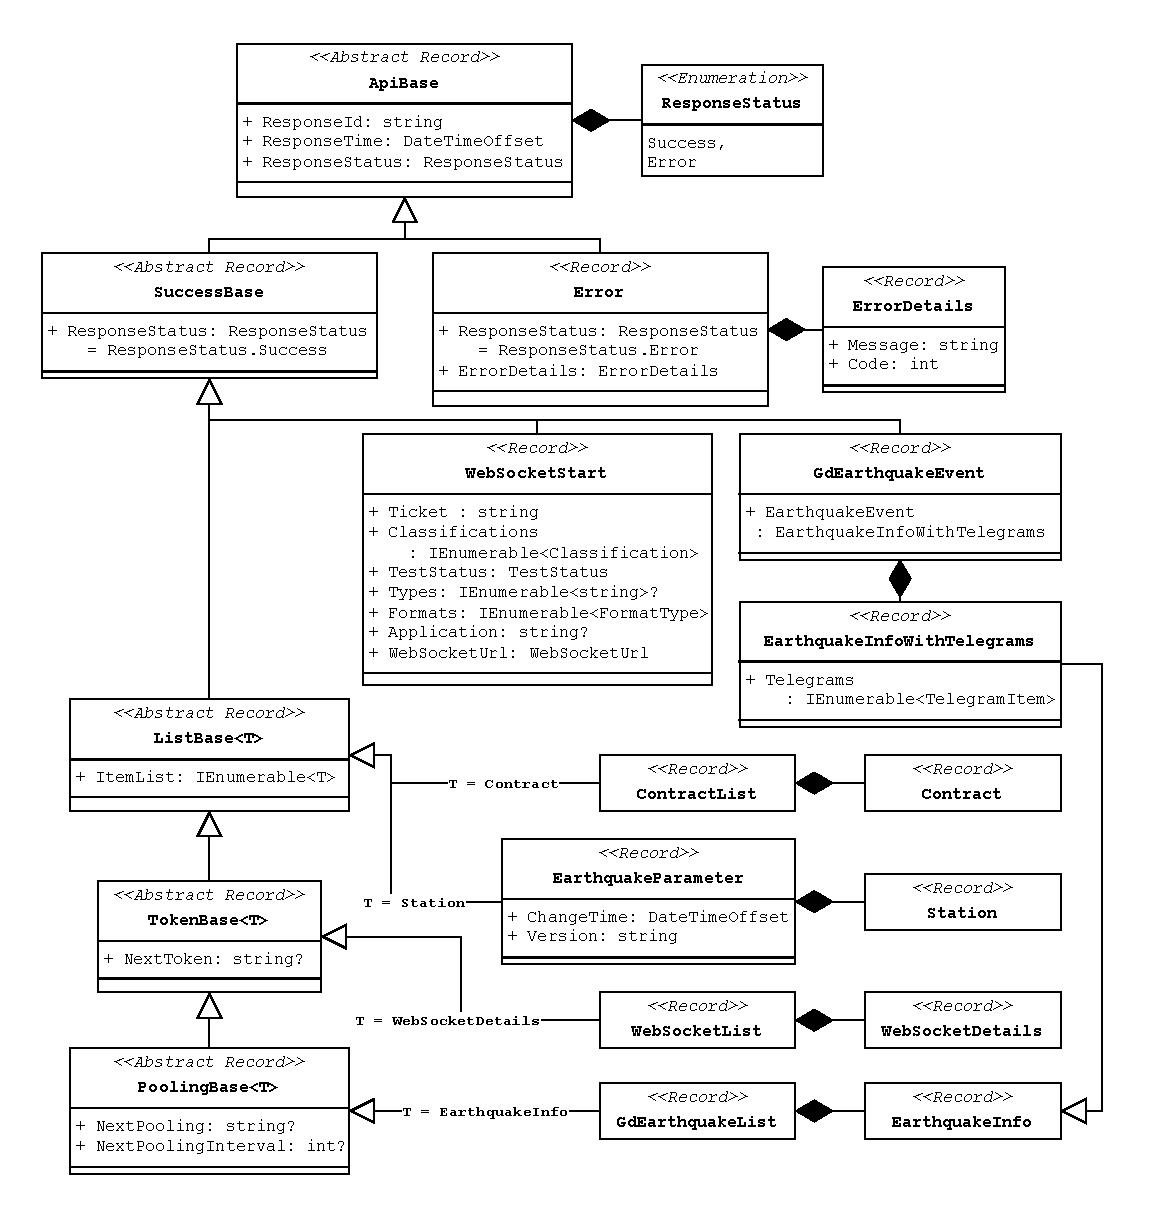
\includegraphics[width=\linewidth]{class-diagram-dmdata-api-dto.pdf}
    \caption{Class Diagram for DTOs for API Calls}
    \label{fig:class-diagram-dmdata-api-dto}
\end{figure}

Most other parts of the DTOs for API Calls is just simply the use of composition as modelled by the DM-D.S.S. API documentation, and the use of enumerations to model 'finitely many values'.

\subsubsection{Telegrams}

Similar to the API calls, a base class \Code{Head} which contains the head information of the telegram is modelled. And then, classes are inherited from this class to provide the body part of the telegram. The reason why \Code{Head} is not abstract, is because telegrams would have to be deserialised to it first and find the JSON schema, and then re-deserialised to the specific type of the telegram.

This is reflected in Figure \ref{fig:class-diagram-dmdata-telegram-dto} which shows a clear use of \textbf{inheritance and composition}.

\begin{figure}[htp]
    \centering
    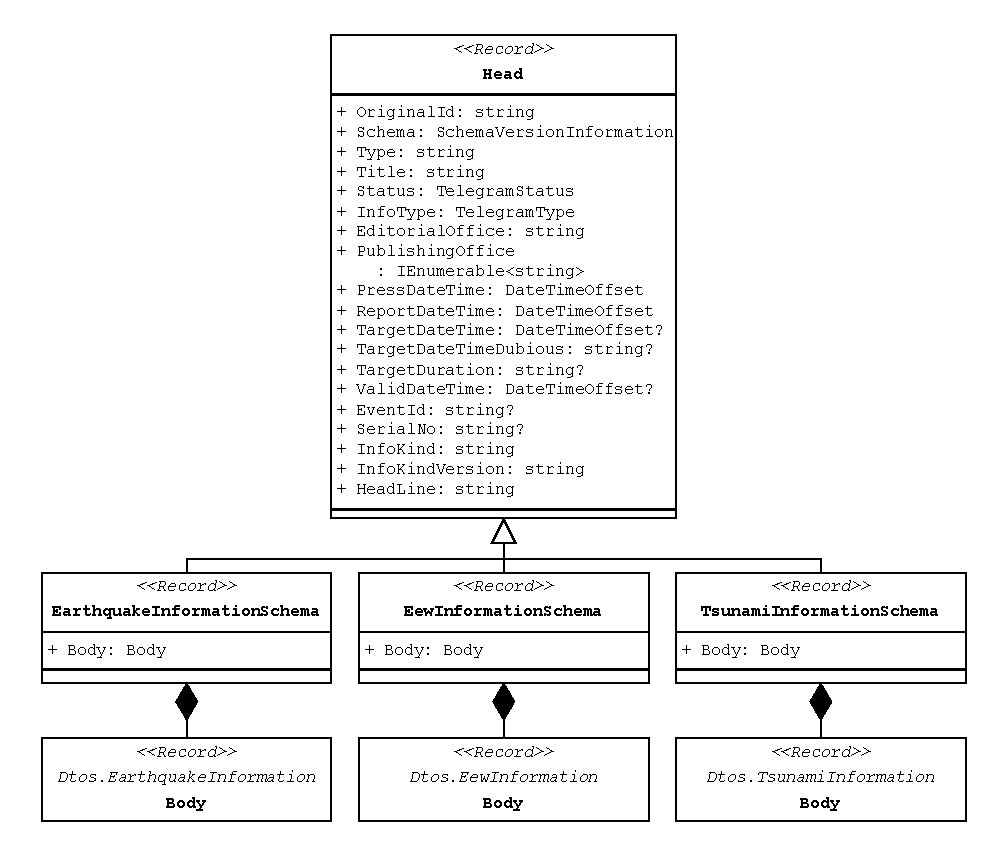
\includegraphics[width=\linewidth]{class-diagram-dmdata-telegram-dto.pdf}
    \caption{Class Diagram for DTOs for Telegrams}
    \label{fig:class-diagram-dmdata-telegram-dto}
\end{figure}

Otherwise, this it simply the use of composition as modelled by the DM-D.S.S. JSON Documentation \autocite{dmdata-references-telegram}.

\section{Hardware and Software Requirements}

Table \ref{tab:hardware-spec} outlines the expected basic hardware requirements for the application.

\begin{table}[htp]
    \centering

    \begin{tabular}{ccc}
        Type               & Minimum                        & Recommended                     \\
        \hline
        RAM                & 4 GB                           & 8 GB                            \\
        Storage Device     & HDD                            & SSD                             \\
        CPU                & Intel Core 8th Gen (or equiv.) & Intel Core 10th Gen (or equiv.) \\
        Display Resolution & 720p                           & 1080p                           \\
        Display Size       & 9''                            & 12''
    \end{tabular}
    \caption{Hardware Specification for App}
    \label{tab:hardware-spec}
\end{table}

The amount of RAM is due to the amount of data that is processed (and considering other applications running as well). Storage space is not a substantial requirement of this application, while the CPU has to be of high standards to process all the data. To display the application properly (with appropriate size), a display of 1080p 12'' is recommended.

It will be able to run on up-to-date Windows, macOS and Linux distributions (both x64 and ARM) due to the cross-platform nature of .NET, but out-of-date x86 platforms will not be explicitly supported.

The author uses a macOS 15 (beta) machine with 2.5K 13'' display, Intel Core i5-1038NG7 (with Intel Iris Plus Graphics) and 16 GB of RAM (MacBook Pro 2020, 4 Thunderbolt Ports) and a Windows 11 (beta) machine with 2.5K 15'' display, AMD Ryzen 7 5800H and 32 GB of RAM (with RTX 3070 for Laptop) (Legion R9000K 2021) to test the application, and with 2.5K 24'' external display as well. An Ubuntu 22.04 virtual machine will be used to test the compatibility for Linux systems.

The application will be self-contained (i.e. comes with .NET runtime) to prevent the user from unnecessary technical complications.

The device needs to have stable connection to the internet using Wi-Fi/Ethernet/other means, to establish connection with the relevant APIs.